\section{Systematics}
\label{sec:syst}
The fit's main goal is to minimise impact of systematic parameters for T2K-SK oscillation analyses by using near-detector data. The shared parameters between ND280 and SK are the neutrino flux parameters (since T2K and SK are in the same neutrino ``beamline''), and neutrino-nucleus interaction parameters. The ``nuisance parameters'' can be considered as the ND280 detector parameters and cross-section parameters that are parametrised as only effective on Carbon. As such, there are many ``parameters of interest'', which the following section covers.

The sources of systematics enter the fit by changing the prediction by shape and/or normalisation, and in most cases the fit incurs a likelihood penalty for moving parameters away from their priors. The penalty takes two forms: either Gaussian or a constant. In the case where there is firm reason to believe a parameter is constrained from other sources, the Gaussian penalty is imposed. When external data or recent model development and similar indicate lacking or conflicting knowledge of a parameter, a flat prior is chosen.

For the Gaussian penalty we have
\begin{equation}
	-2\log\mathcal{L}_\text{Penalty} = (X_i-\mu_i) \left(\mathbf{V}\right)^{-1}_{i,j} (X_j-\mu_j)
\end{equation}
for parameter $i$, with current fit values $X_i$, priors $\mu_i$ and covariance matrix $\mathbf{V}$, and for a flat penalty we have
\begin{equation}
	-2\log\mathcal{L}_\text{Penalty} = C
\end{equation}
where $C$ is a constant.

\subsection{Flux}
\label{subsec:syst_flux}
The flux systematics contain uncertainties from all sources going into the neutrino flux prediction. They are primarily split into six categories:
\begin{itemize}
	\item Hadron interaction uncertainties
	\item Proton beam profile and off-axis angle
	\item Horn current and field
	\item Horn and target alignment
	\item Materials modelling
	\item Number of protons on target
\end{itemize}

The software suite for the beam simulation consists of FLUKA2011 \cite{fluka2008_1, fluka2008_2, fluka2011} which simulates hadronic interactions in target and baffle, JNUBEAM (GEANT3-based \cite{geant3}) which simulates the geometry and tracking, and GCALOR \cite{gcalor} which simulates hadronic re-interactions and is used as a cross-check for FLUKA. Full details are found elsewhere \cite{t2k_beam, t2k_tn_flux}.

The simulations are updated each year to improve the modelling, often taking additional data in to account. An example of such is using the dedicated NA61/SHINE T2K replica target data \cite{NA61_pions_rep} to tune the hadron production model at the T2K beam target, and including results from the HARP experiment \cite{harp}.

The effects on the fractional error for the ND280 neutrino flux prediction is shown in \autoref{fig:flux_uncert_fhc} for FHC running and \autoref{fig:flux_uncert_rhc} for RHC running. The uncertainties are $\sim10\%$ in the flux peak region and is dominated by the hadron interaction uncertainties, which in turn consists primarily of multiplicity, pion rescattering and interaction length uncertainties. The proton beam profile and off-axis angle become important shortly after the flux peak at about 1 GeV for the right-sign component of the flux.

\begin{figure}[h]
	\begin{subfigure}[t]{0.42\textwidth}
		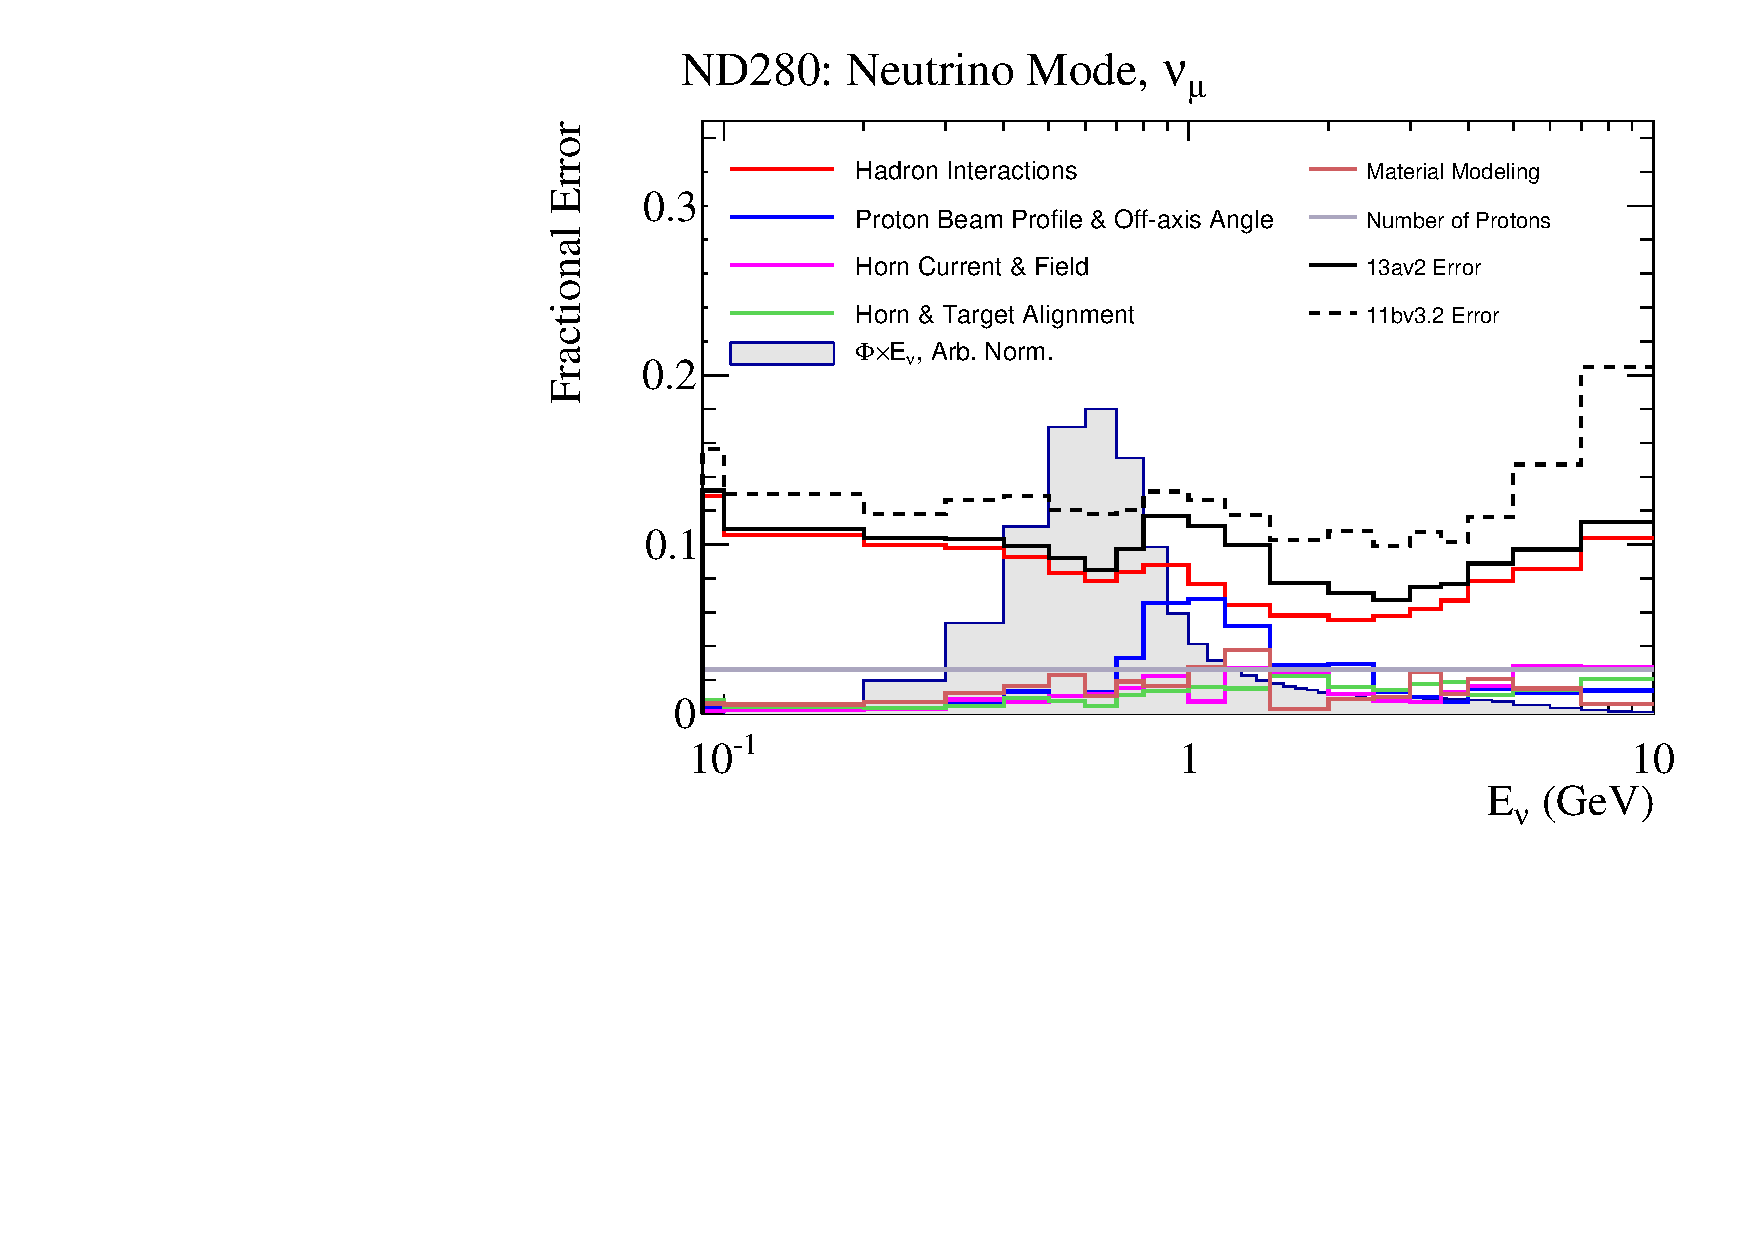
\includegraphics[width=\textwidth, trim={0mm 0mm 0mm 0mm}, clip,page=1]{figures/flux/total_err_nd5_numode_numu}
	\end{subfigure}
	\begin{subfigure}[t]{0.42\textwidth}
		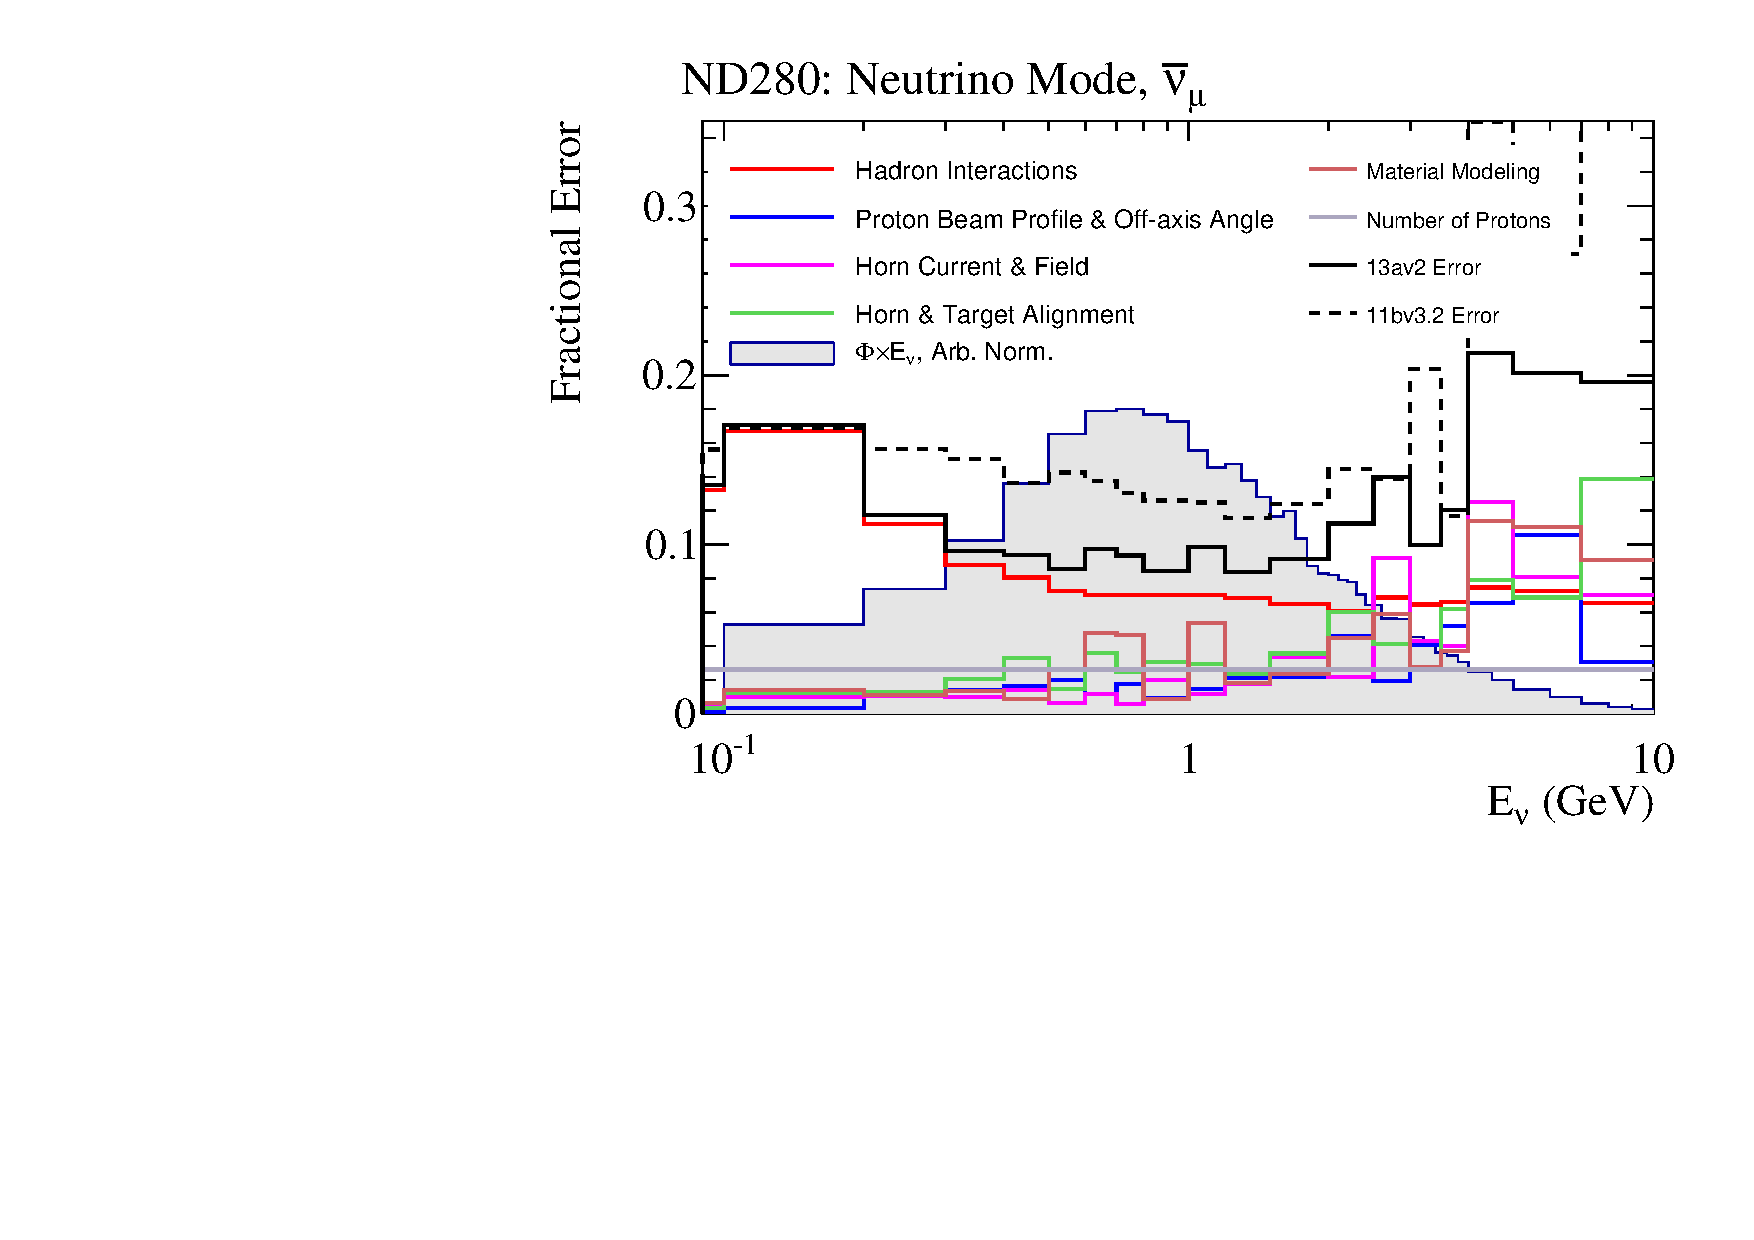
\includegraphics[width=\textwidth, trim={0mm 0mm 0mm 0mm}, clip,page=1]{figures/flux/total_err_nd5_numode_numub}
	\end{subfigure}

	\begin{subfigure}[t]{0.42\textwidth}
		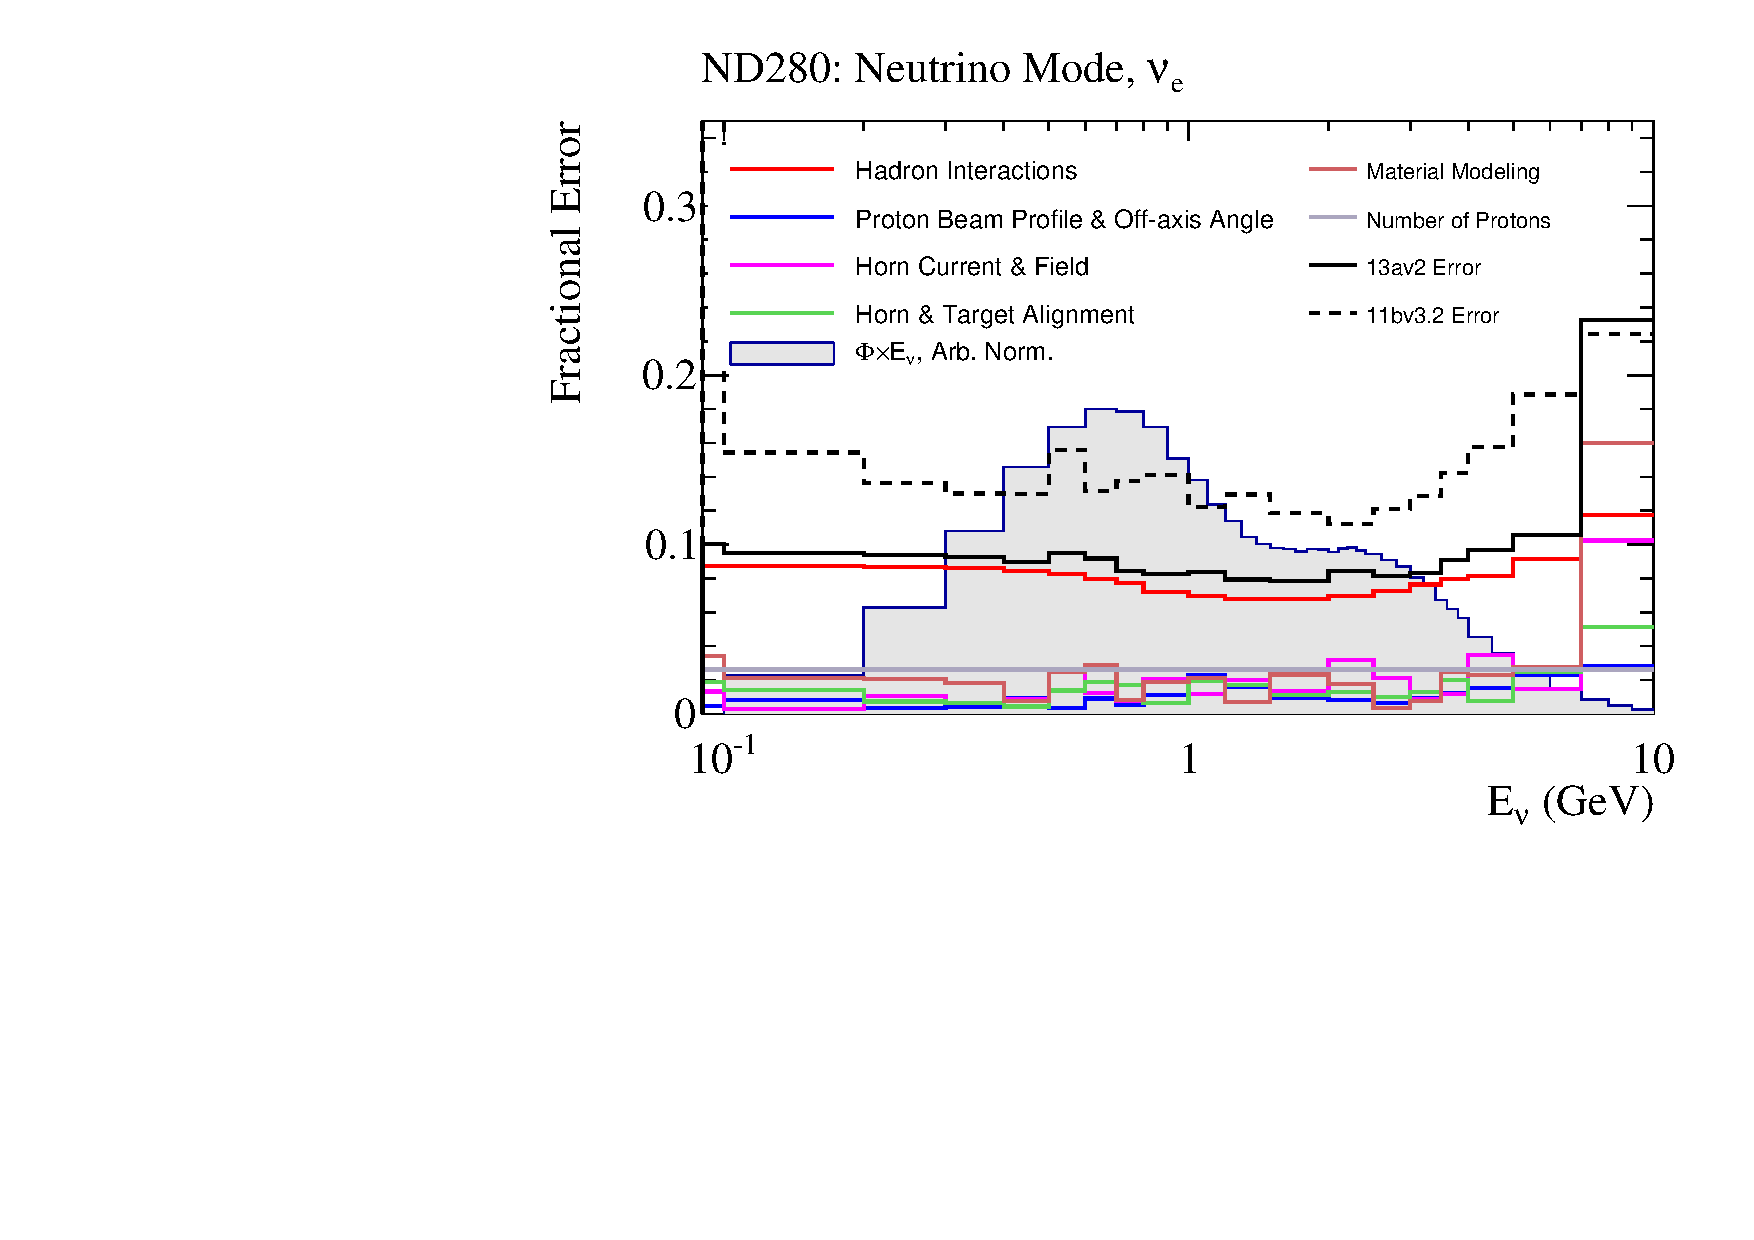
\includegraphics[width=\textwidth, trim={0mm 0mm 0mm 0mm}, clip,page=1]{figures/flux/total_err_nd5_numode_nue}
	\end{subfigure}
	\begin{subfigure}[t]{0.42\textwidth}
		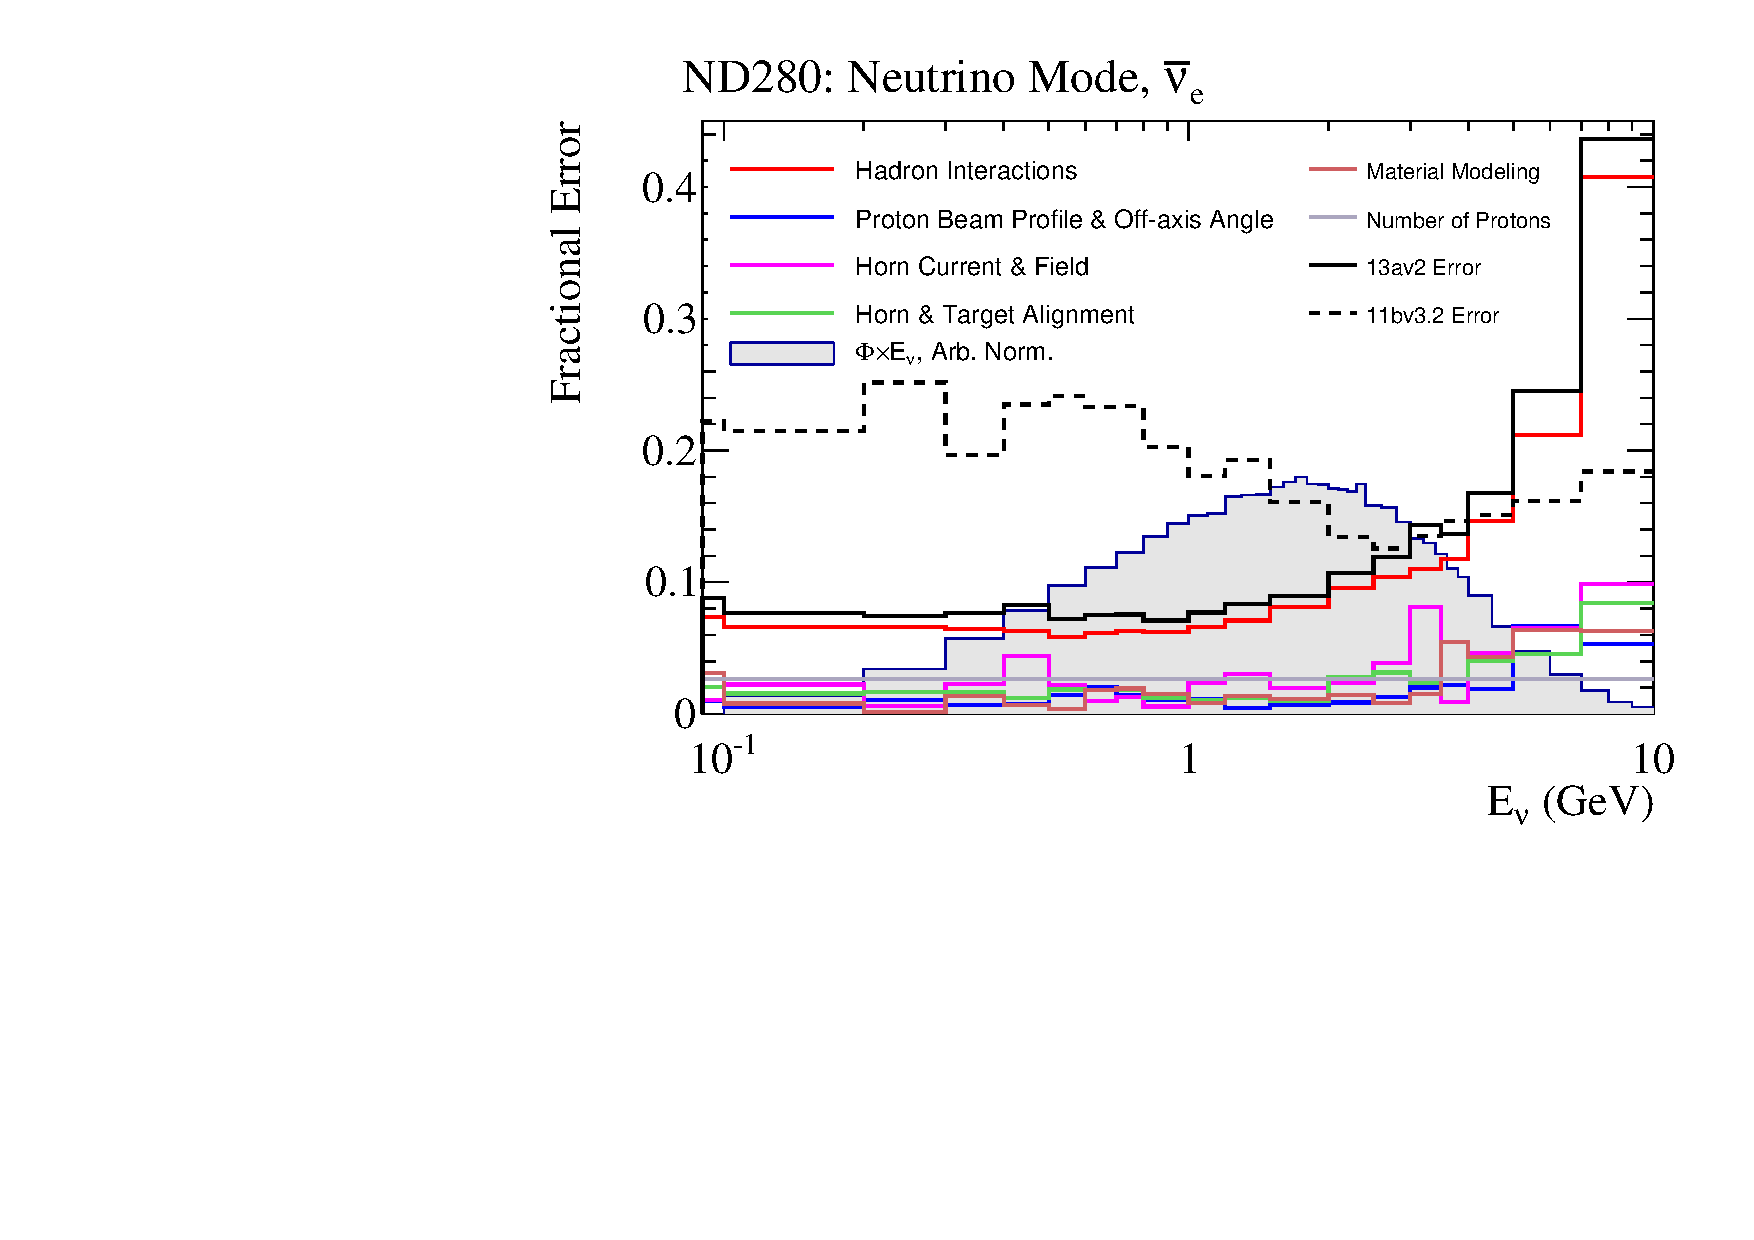
\includegraphics[width=\textwidth, trim={0mm 0mm 0mm 0mm}, clip,page=1]{figures/flux/total_err_nd5_numode_nueb}
	\end{subfigure}
	\caption{FHC flux uncertainties, ``13av2 Error'' is used for this analysis}
	\label{fig:flux_uncert_fhc}
\end{figure}

\begin{figure}[h]
	\begin{subfigure}[t]{0.42\textwidth}
		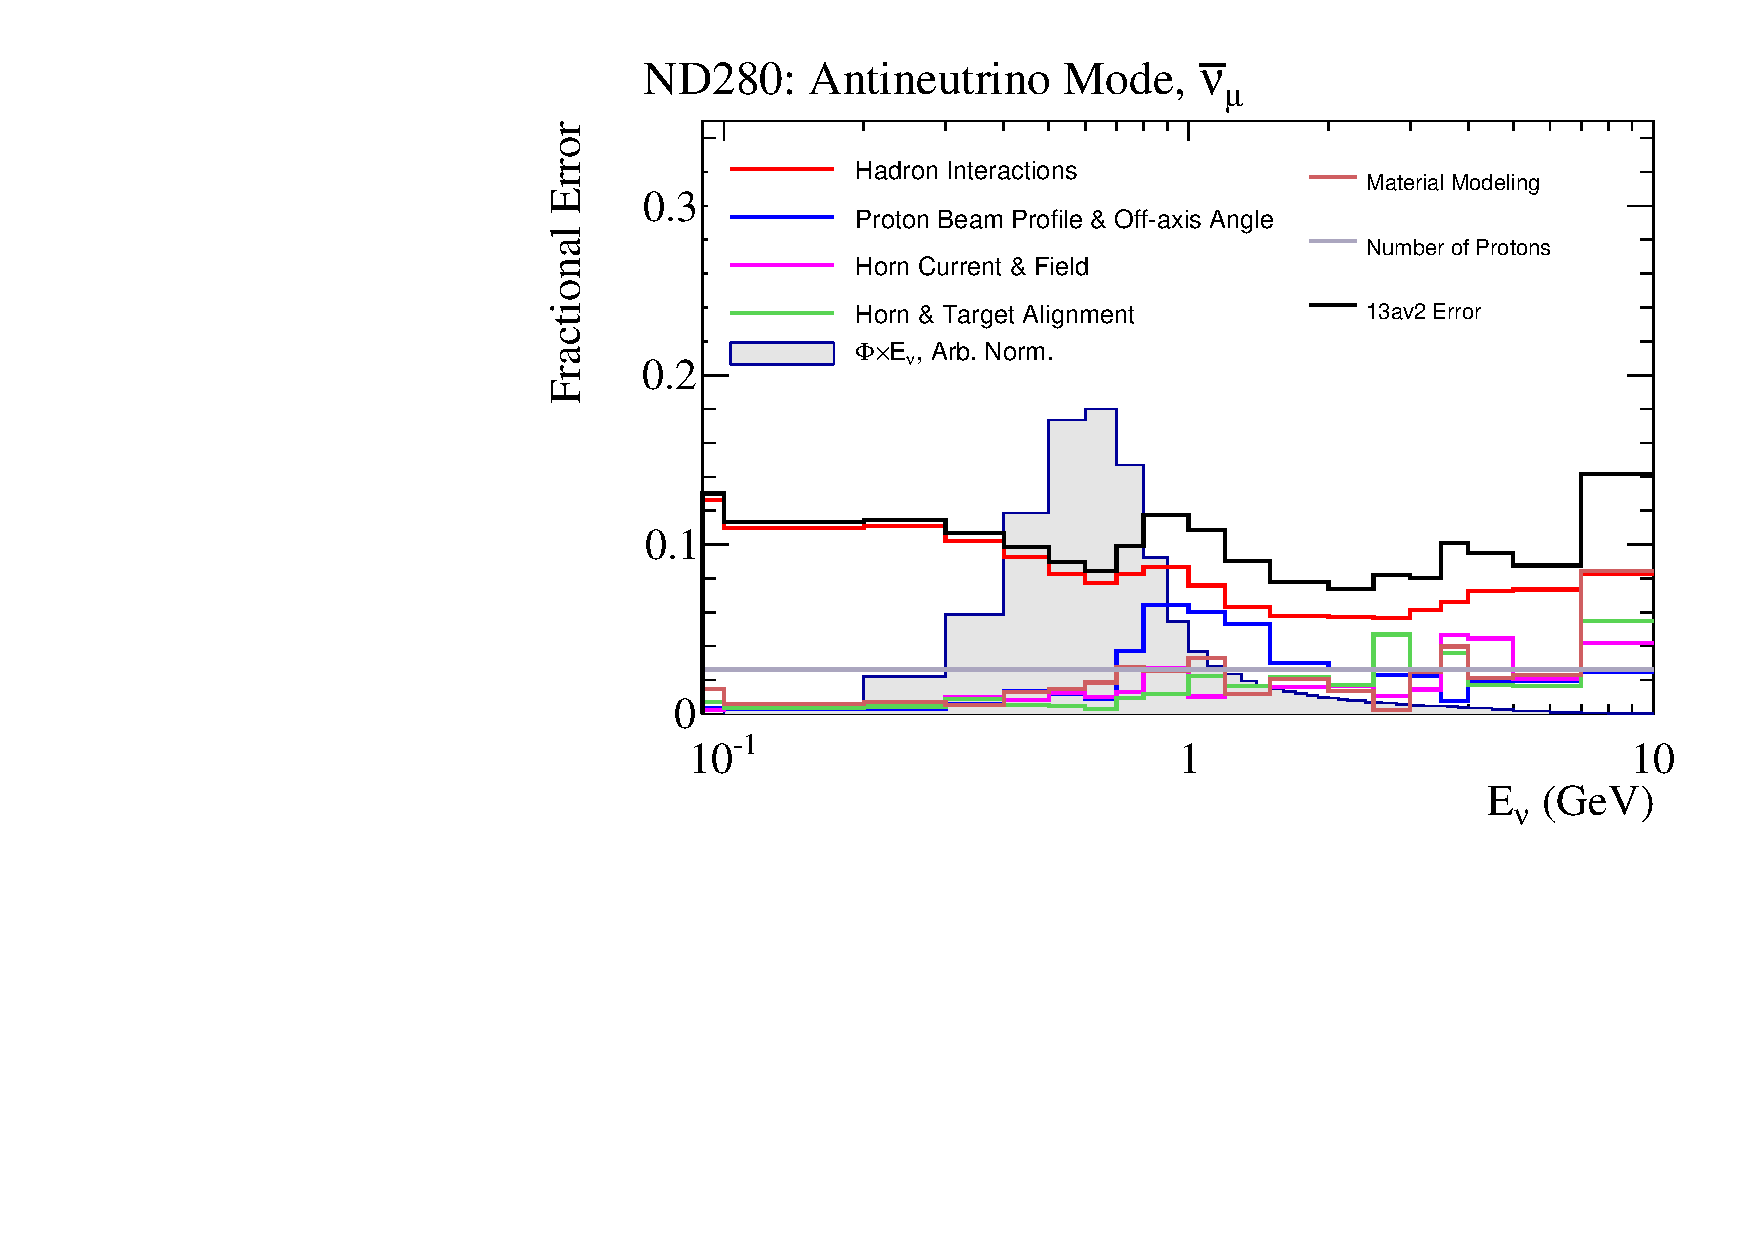
\includegraphics[width=\textwidth, trim={0mm 0mm 0mm 0mm}, clip,page=1]{figures/flux/total_err_nd5_anumode_numub}
	\end{subfigure}
	\begin{subfigure}[t]{0.42\textwidth}
		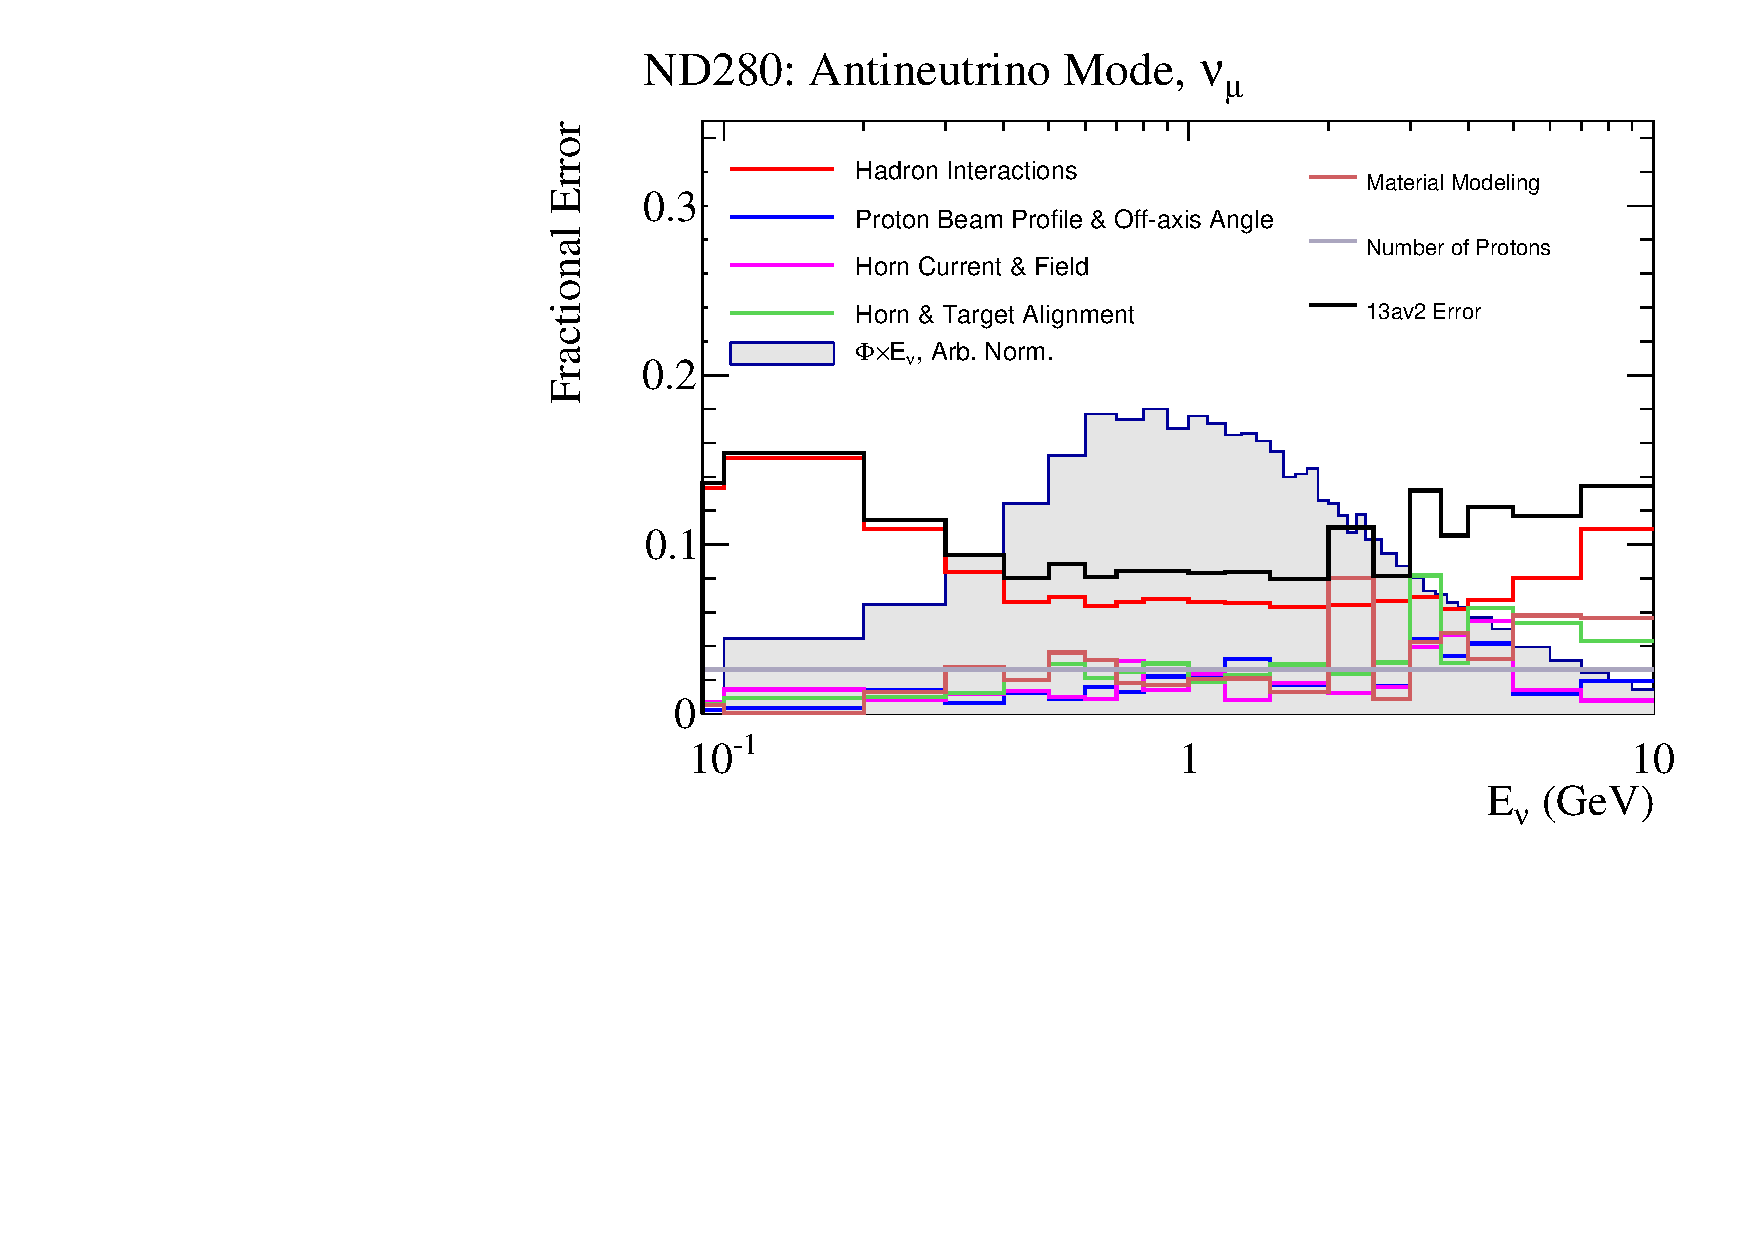
\includegraphics[width=\textwidth, trim={0mm 0mm 0mm 0mm}, clip,page=1]{figures/flux/total_err_nd5_anumode_numu}
	\end{subfigure}

	\begin{subfigure}[t]{0.42\textwidth}
		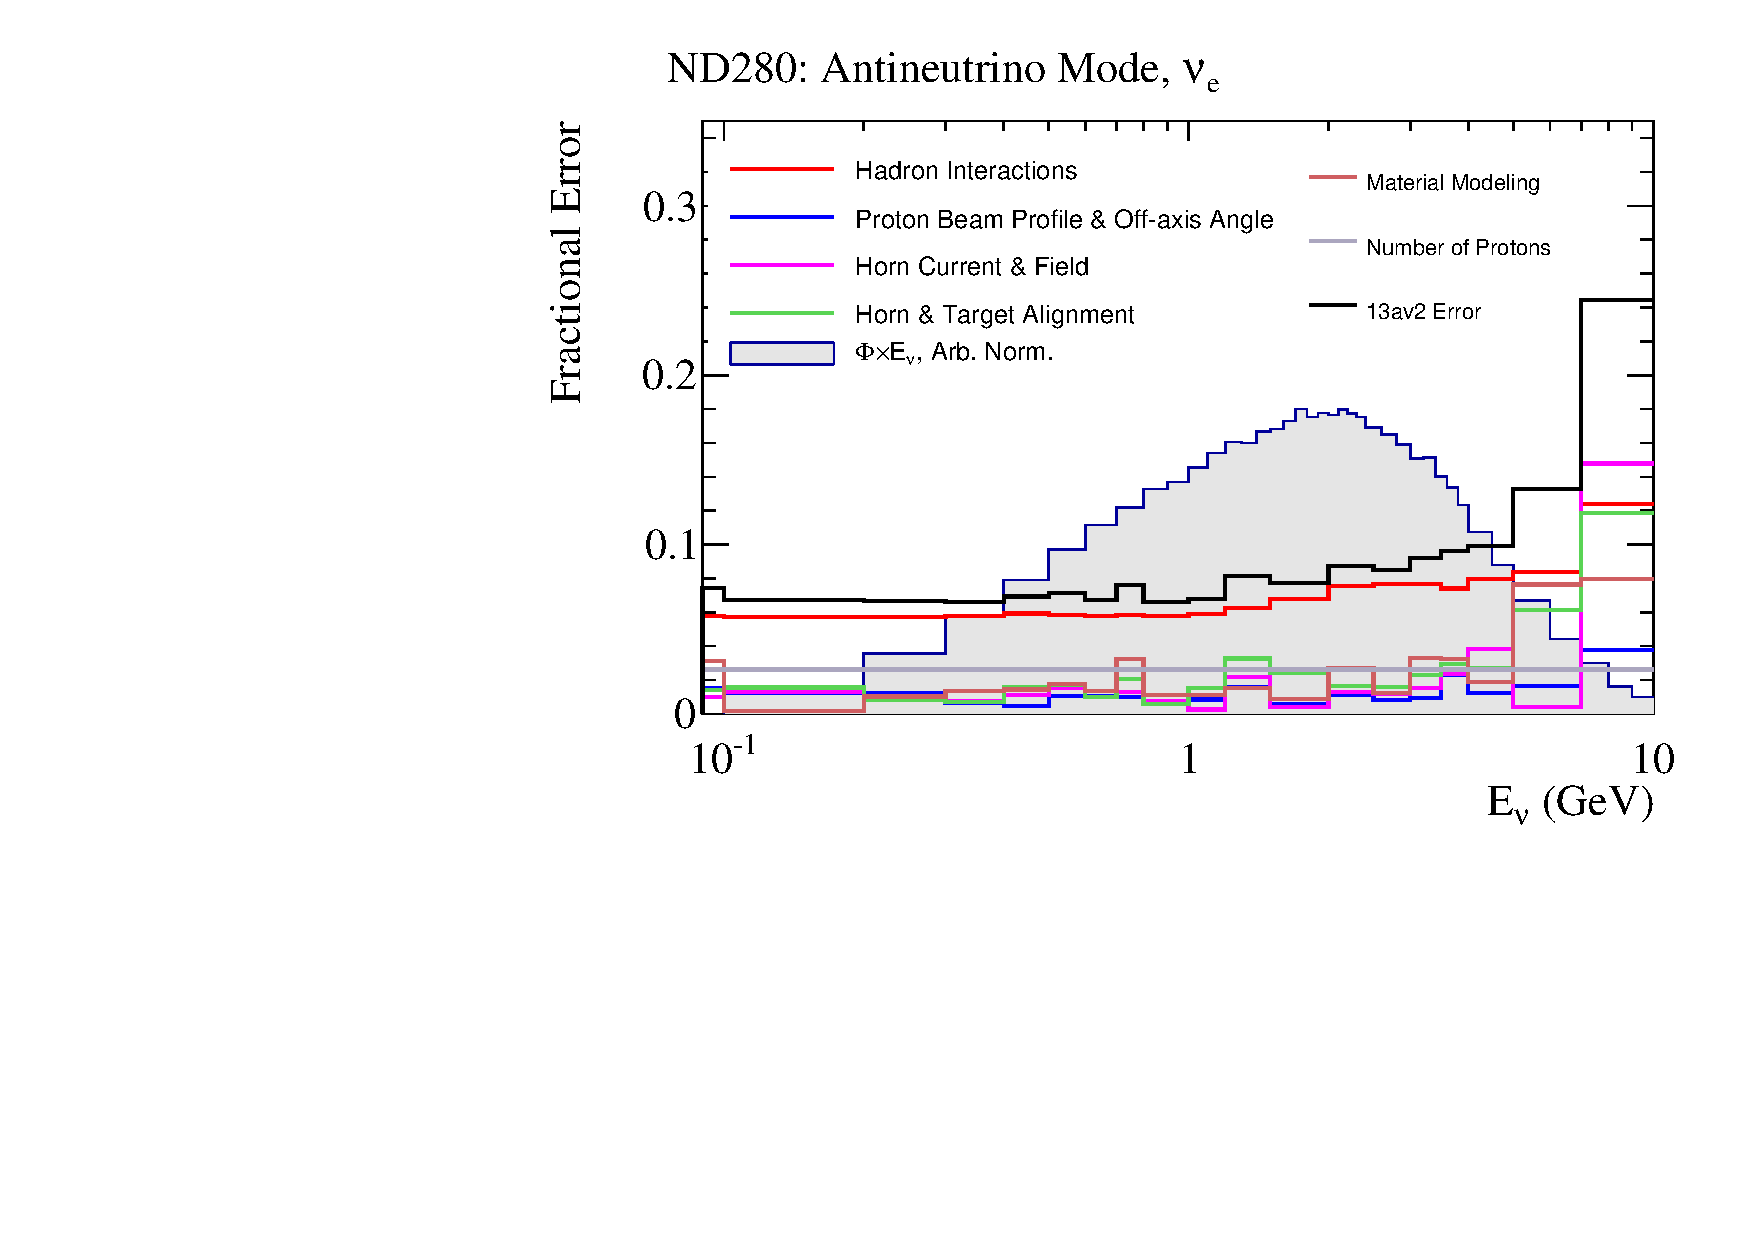
\includegraphics[width=\textwidth, trim={0mm 0mm 0mm 0mm}, clip,page=1]{figures/flux/total_err_nd5_anumode_nue}
	\end{subfigure}
	\begin{subfigure}[t]{0.42\textwidth}
		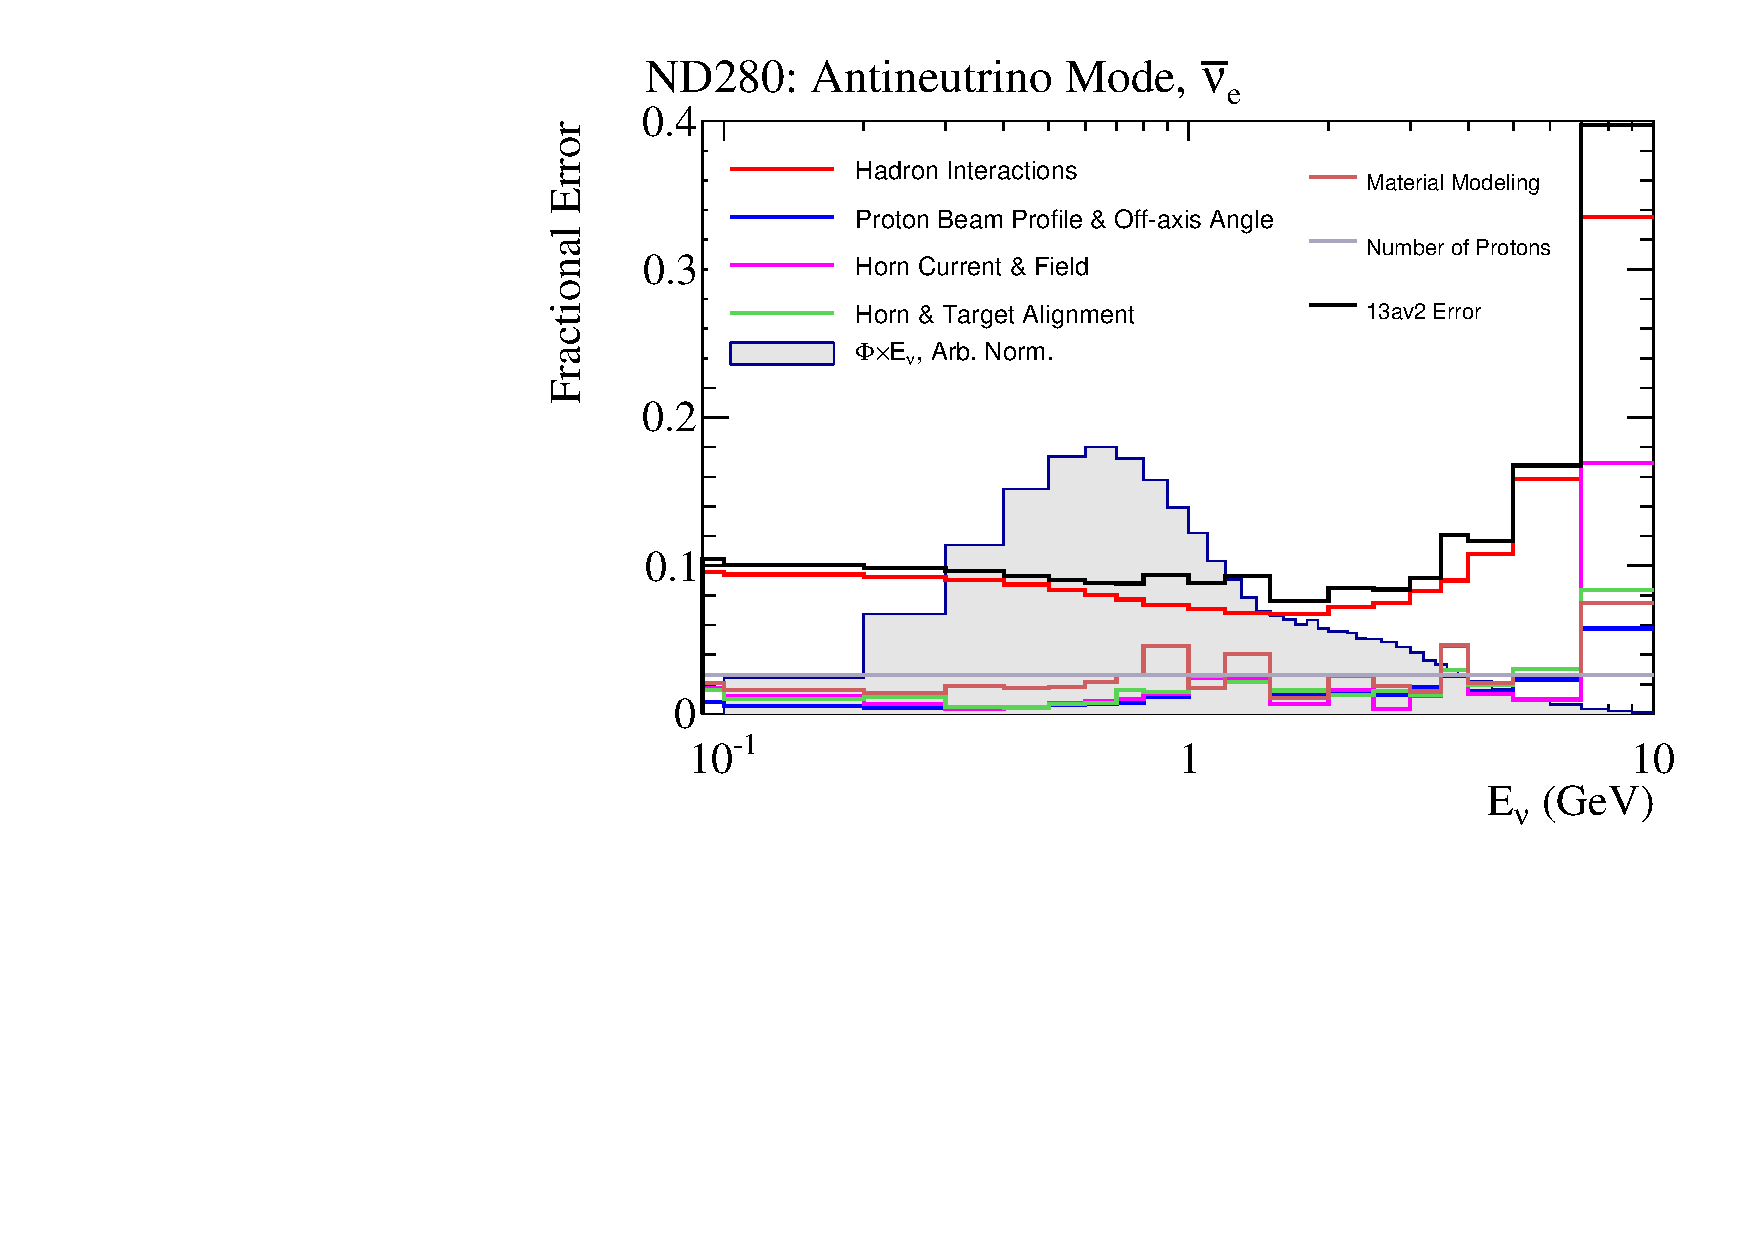
\includegraphics[width=\textwidth, trim={0mm 0mm 0mm 0mm}, clip,page=1]{figures/flux/total_err_nd5_anumode_nueb}
	\end{subfigure}
\caption{RHC flux uncertainties, ``13av2 Error'' is used for this analysis}
\label{fig:flux_uncert_rhc}
\end{figure}

Importantly, the hadronic interaction uncertainty is reducible by improved modelling and tuning to carefully selected relevant hadron production data, which is the main method of reducing the flux uncertainty at T2K. An example of such an effort is the black dashed line and the black solid line in \autoref{fig:flux_uncert_fhc}, which shows the reduction in flux uncertainty from 2014 to 2015 analyses. Additionally, new beam profile monitors aid in reducing the proton beam profile and off-axis angle uncertainties.

The flux systematics enter the near-detector and oscillation analyses as bin-by-bin normalisations in $E_\nu^\text{True}$ for four different neutrino species (\numu, \numubar, \nue, \nuebar), for each running mode (FHC, RHC), for each detector (ND280, SK). The binning is chosen to reflect the magnitude of the neutrino flux and the changing shape but simultaneously keeping the number of parameters relatively low. The right-sign and wrong-sign species have the same binning, so ND280 FHC \numu is binned as ND280 RHC \numubar:
\begin{itemize}
	\item ND280, SK FHC \numu; ND280, SK RHC \numubar, :\\
	$E_\nu^{true}$: 0, 0.4, 0.5, 0.6, 0.7, 1, 1.5, 2.5, 3.5, 5, 7, 30
	
	\item ND280, SK FHC \numubar; ND280, SK RHC \numu:\\
	$E_\nu^{true}$: 0, 0.7, 1, 1.5, 2.5, 30
	
	\item ND280, SK FHC \nue; ND280, SK RHC \nuebar:\\
	$E_\nu^{true}$: 0, 0.5, 0.7, 0.8, 1.5, 2.5, 4, 30
	
	\item ND280, SK FHC \nuebar; ND280, SK RHC \nue:\\
	$E_\nu^{true}$: 0, 2.5, 30
\end{itemize}
This procedure brings the total number of flux parameters to 100: 50 for ND280 and 50 for SK. The SK flux parameters are not directly constrained in the near-detector fit: however because of the very strong ND280-SK flux correlations, the constraint on the ND280 flux parameters from ND280 data indirectly moves SK flux parameters. Hence, all 100 parameters are fit at ND280.

The central values and bin-by-bin uncertainties are highly correlated so the likelihood penalties are evaluated with a covariance matrix, shown in \autoref{fig:flux_cov}.
\begin{figure}[h]
	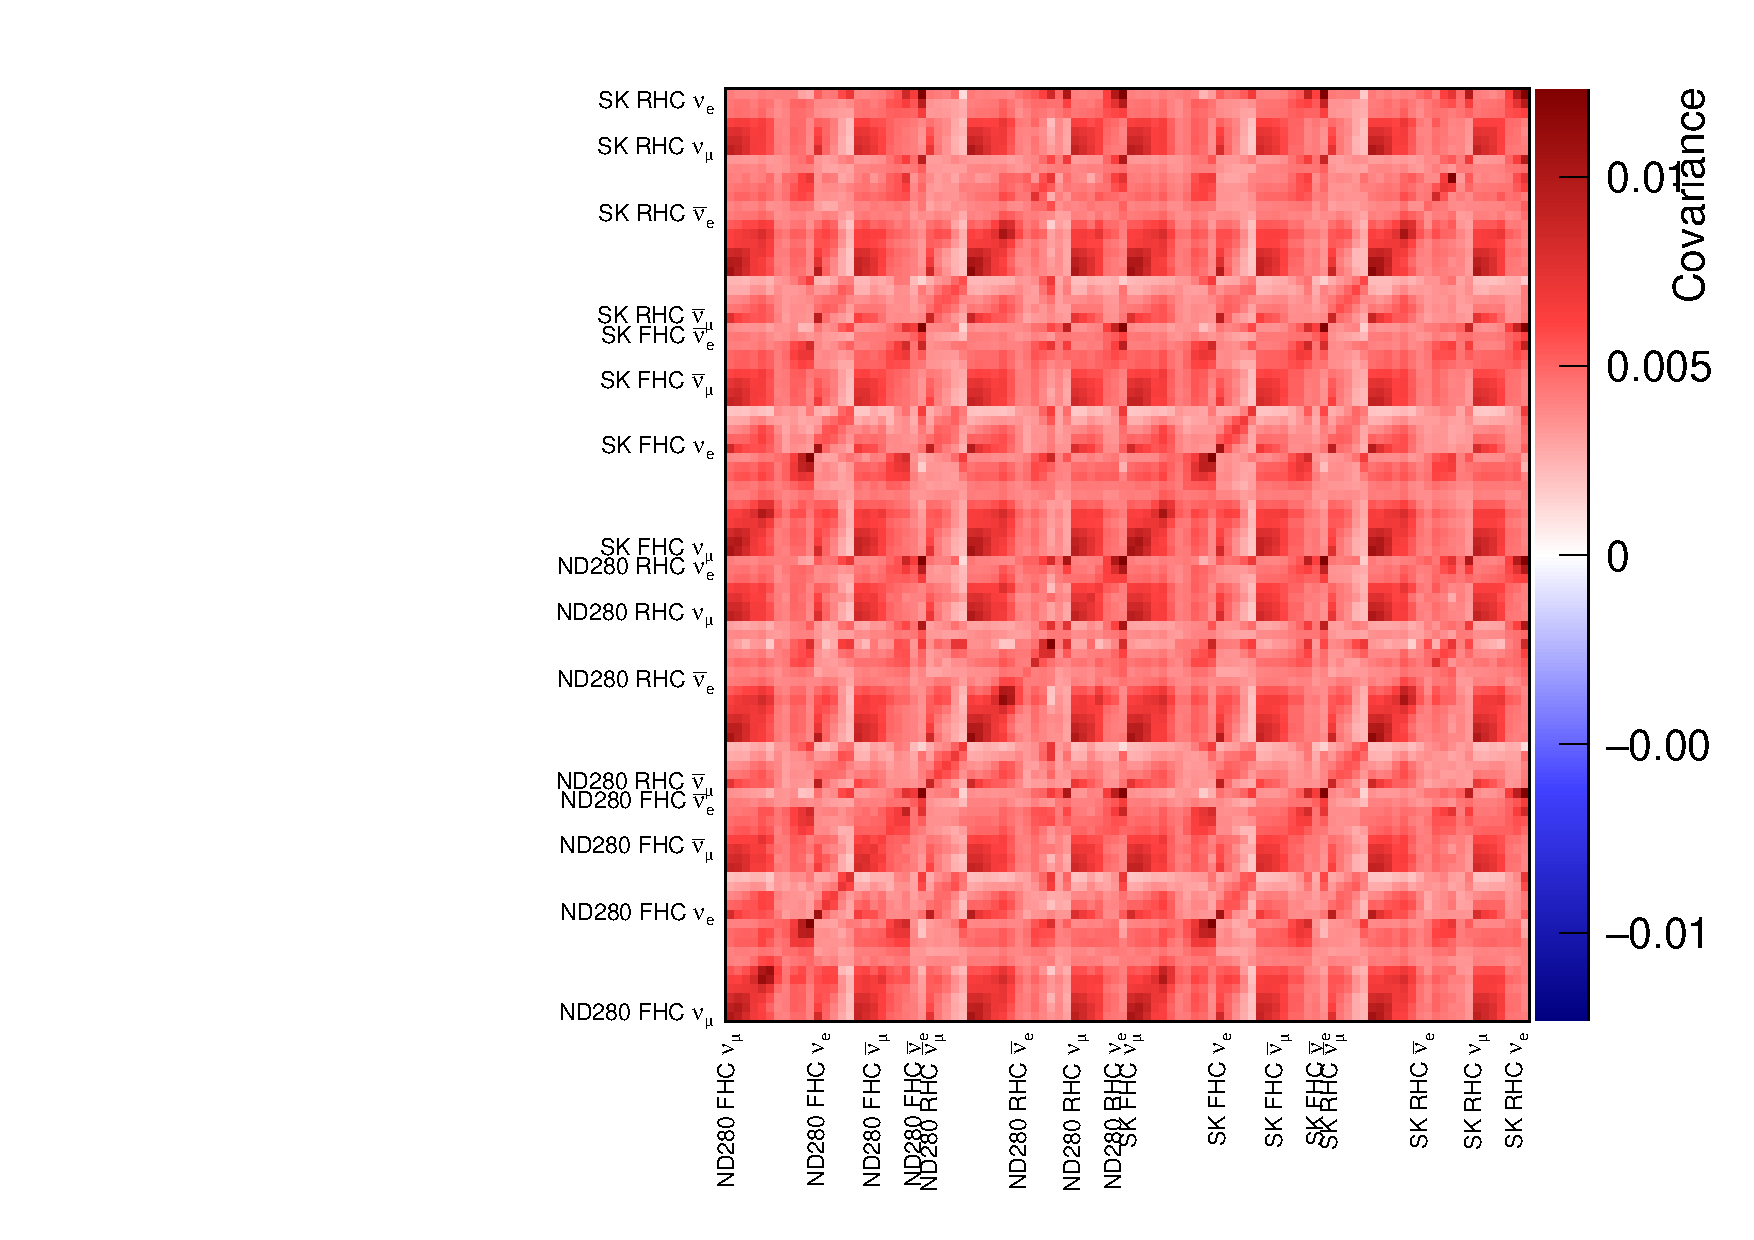
\includegraphics[width=0.45\textwidth, trim={0mm 0mm 0mm 0mm}, clip,page=1]{figures/mach3/inputs/flux_covariance_banff_13av2}
	\caption{13av2 covariance matrix, used in this analysis}
	\label{fig:flux_cov}
\end{figure}

%pi+ to mu+numu 99.9877
%to e+nue 1.23E-4
%Kplus to mu+numu 63.55
%to pi0mu+numu3.353
%to pi0e+nue 5.07
%K0L to pi-mu+numu 27.04
%to pi0e+nue 40.55
%mu+ to e+numubar+nue 100

In addition to the variation systematics above, there is also a nominal flux correction applied to each event as a function of its run period (e.g. run 2a), neutrino specie (e.g. \numubar) and $E_\nu^{\text{True}}$ (e.g. 0.8 GeV). This is present to correct the nominal flux model which the Monte-Carlo was produced with updated measurements. An example from run 4a and run 5b is shown in \autoref{fig:flux_ratio}.
\begin{figure}[h]
	\begin{subfigure}[t]{0.42\textwidth}
		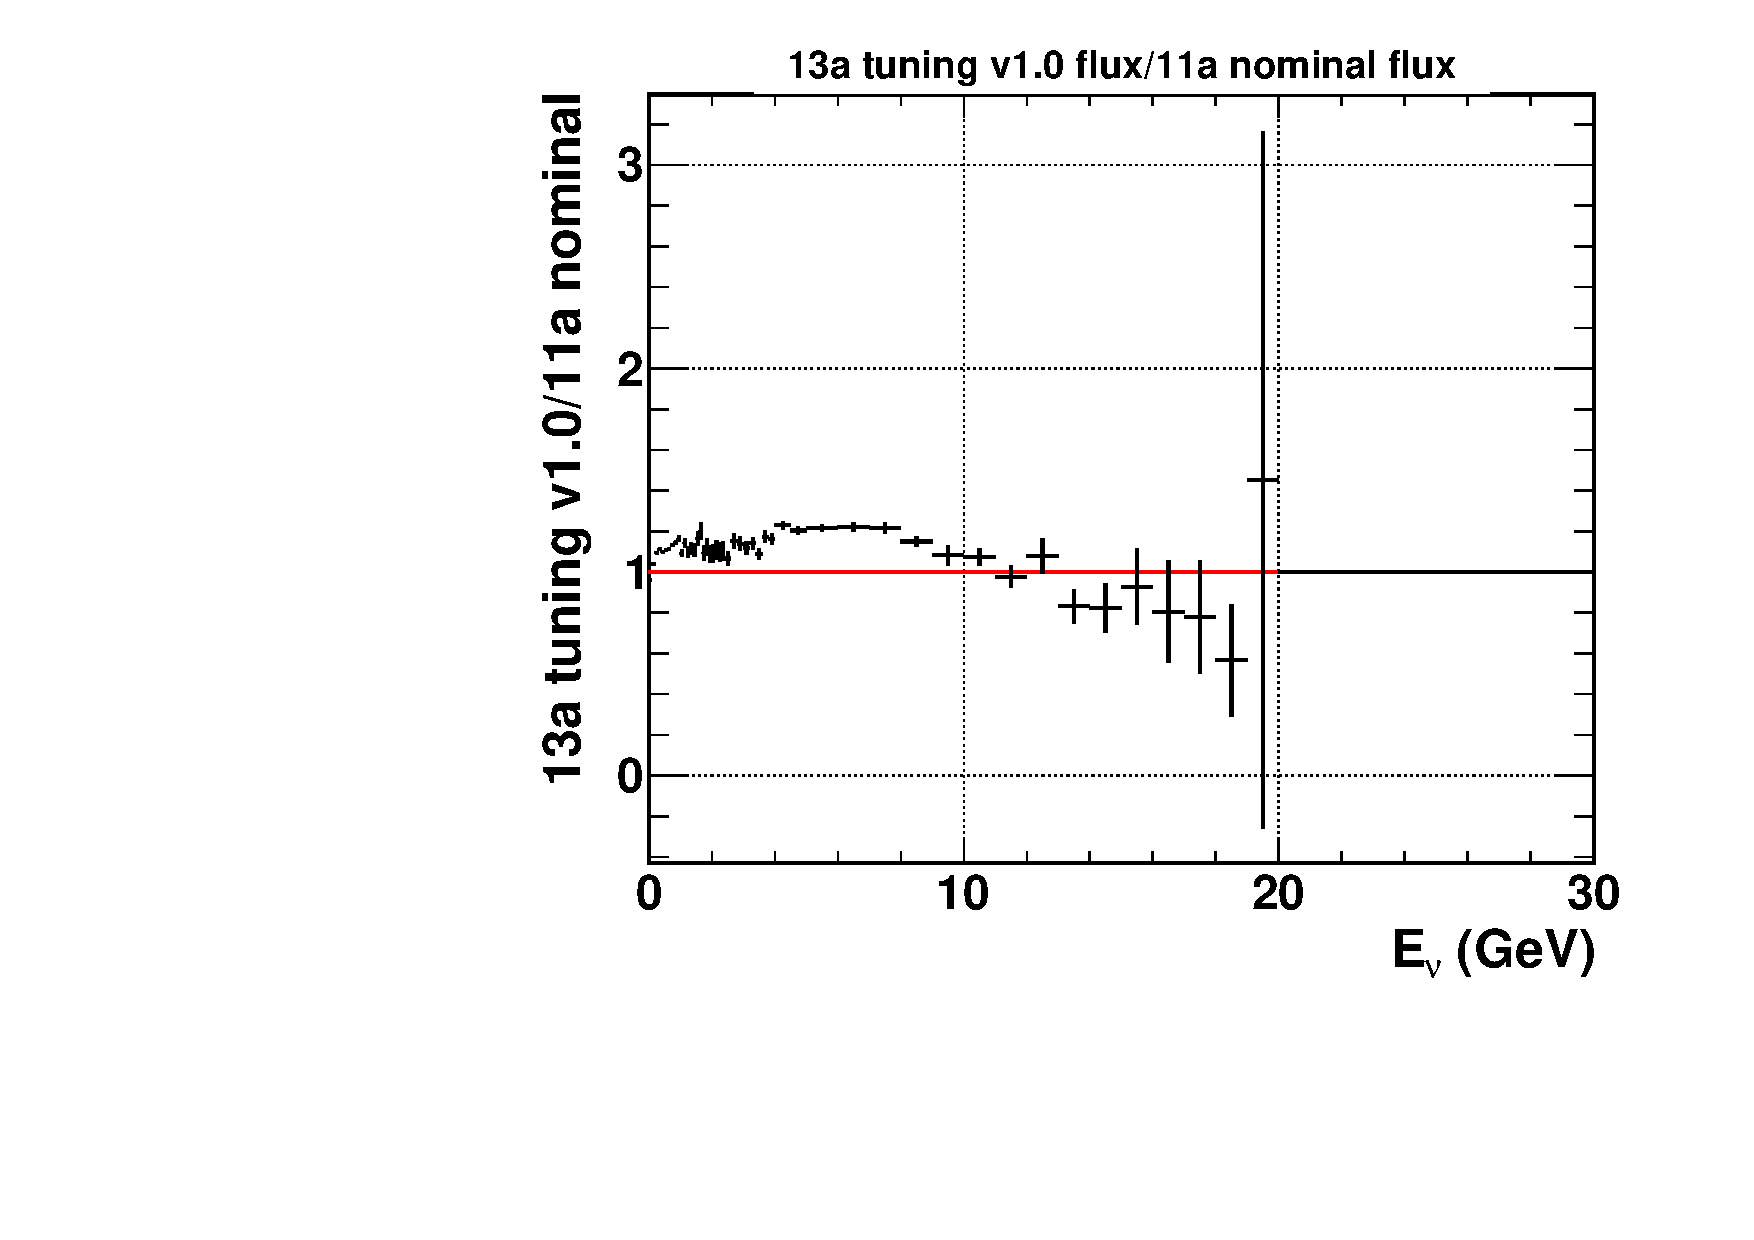
\includegraphics[width=\textwidth, trim={0mm 0mm 0mm 0mm}, clip,page=1]{figures/flux/run4_enu_nd5_13av2_numu_rat}
		\caption{4a \numu}
	\end{subfigure}
	\begin{subfigure}[t]{0.42\textwidth}
		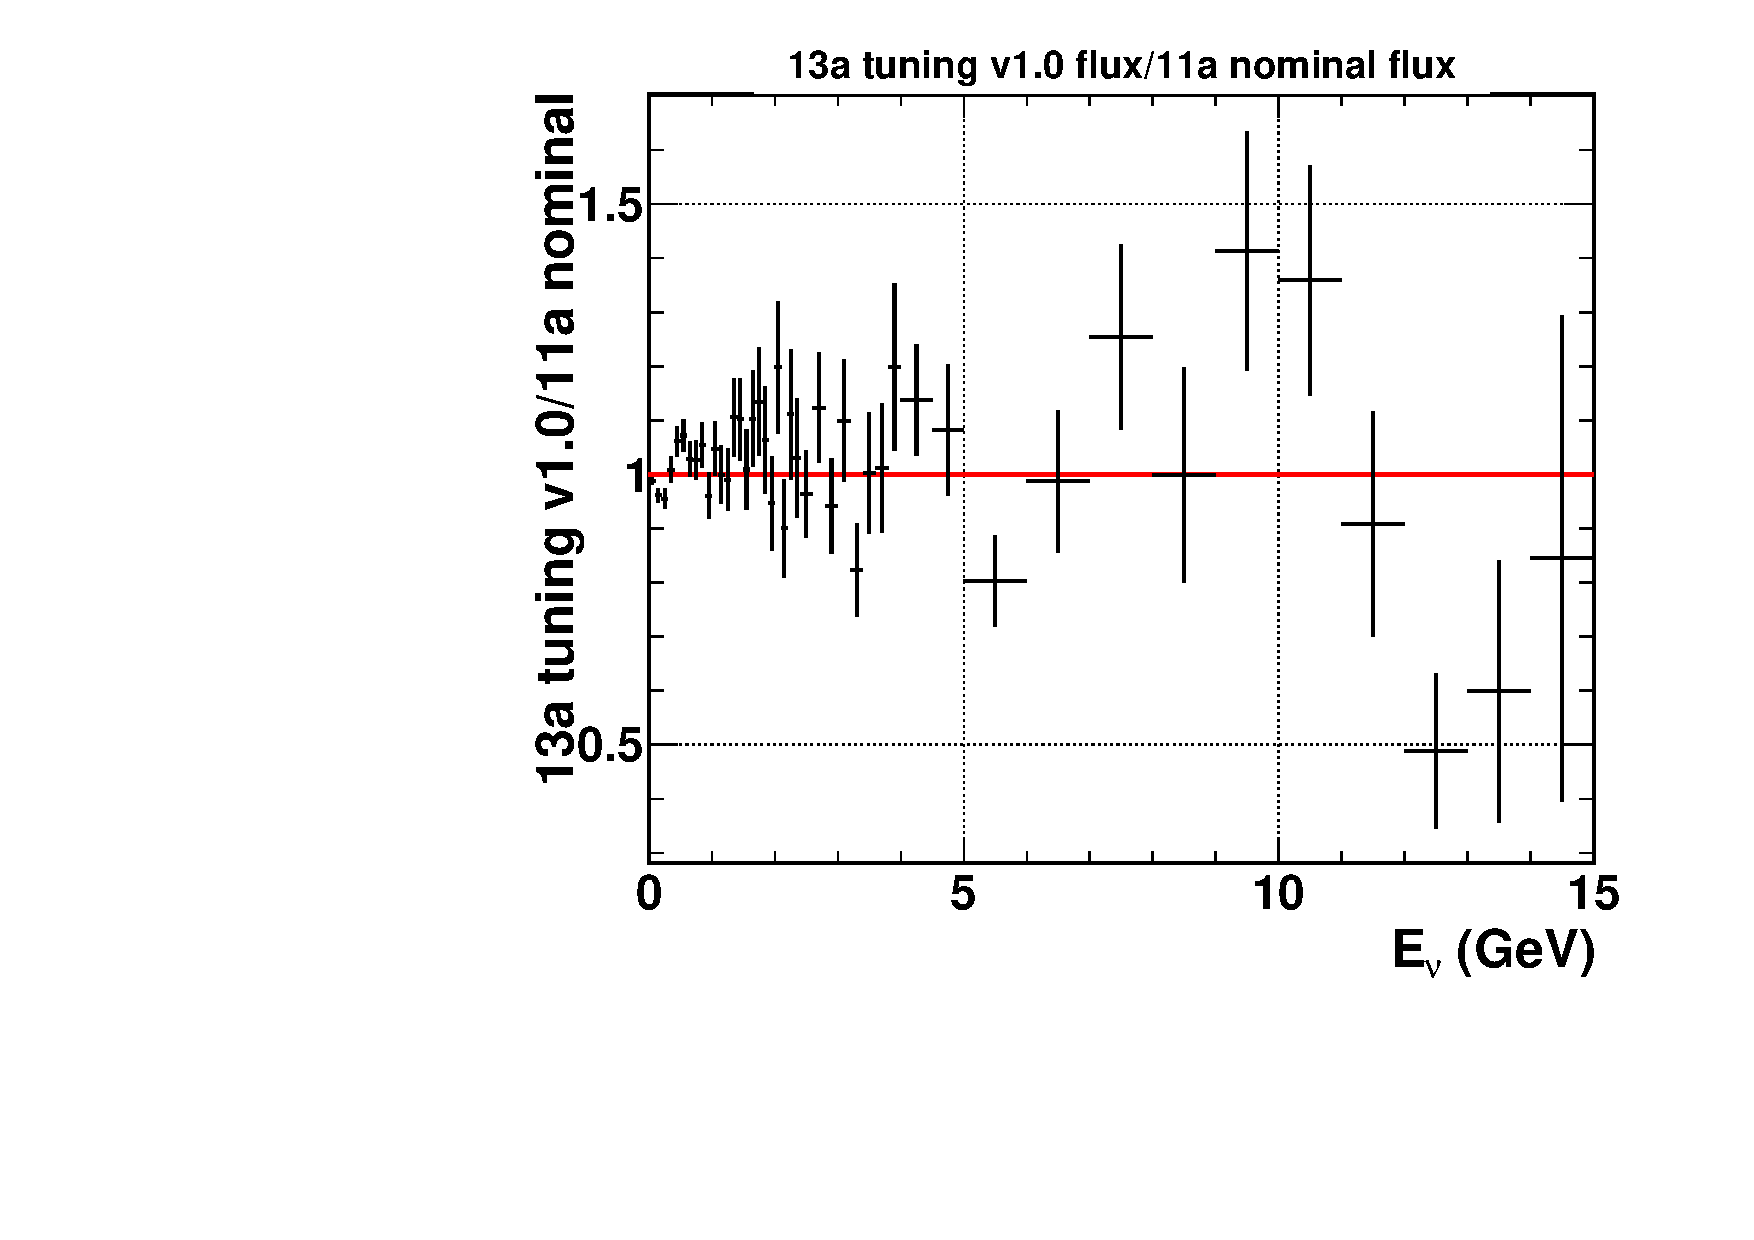
\includegraphics[width=\textwidth, trim={0mm 0mm 0mm 0mm}, clip,page=1]{figures/flux/run5b_enu_nd5_13av2_numubar_rat}
		\caption{5b \numubar}
	\end{subfigure}
	\caption{Nominal flux corrections applied to events in the ND5 tracker plane}
	\label{fig:flux_ratio}
\end{figure}

\subsection{Detector systematics}
\label{subsec:syst_nd280}
The treatment of ND280 detector systematic uncertainties consists of varying the underlying detector systematics, such as TPC PID, FGD PID, TPC Momentum scale and study the impact on the number of predicted events in each \pmu \cosmu bin. 

The parameterisation of near detector systematics are categorised as systematics that purely weight an event as the value changes and systematics that vary the observable event topology. The event weighting can further be broken down into efficiencies (with shapes) and normalisation parameters. When FGD-related systematics are concerned---such as pion tagging by Michel electron identification---the two FGDs have separate implementations to account for geometrical and compositional differences.

The different sources of systematics, their variation type and assumed probability distribution function (PDF) are shown in \autoref{tab:nd280_systs}.
\begin{table}[h]
	\begin{tabular}{l | c c}
	\hline
	\hline
	Systematic						& Variation 	& PDF \\
	\hline
	\multicolumn{3}{l}{\textbf{TPC}} \\
	Magnetic Field Distortions		& Observable 	& Flat \\
	TPC Momentum Scale				& Observable	& Gauss \\
	TPC Momentum Resolution			& Observable	& Gauss \\
	TPC PID							& Observable	& Gauss \\
	TPC Cluster Efficiency			& Efficiency	& Gauss \\
	TPC Tracking Efficiency			& Efficiency	& Gauss \\
	TPC Charge ID Efficiency		& Efficiency	& Gauss \\
	\hline 
	\multicolumn{3}{l}{\textbf{FGD-TPC}} \\
	TPC-FGD Matching Efficiency		& Efficiency	& Gauss \\
	\hline
	\multicolumn{3}{l}{\textbf{FGD}} \\
	FGD PID							& Observable	& Gauss \\
	FGD1-FGD2 Time of Flight		& Observable	& Gauss \\
	FGD Hybrid Tracking Efficiency	& Efficiency	& Gauss \\
	Michel Electron Efficiency		& Efficiency	& Gauss \\
	\hline
	\multicolumn{3}{l}{\textbf{Backgrounds}} \\
	Out-of-Fiducial-Volume			& Normalisation & Gauss \\
	Sand Muons						& Normalisation & Gauss \\
	Pile-Up							& Normalisation	& Gauss \\
	\hline
	\multicolumn{3}{l}{\textbf{MC modelling}} \\
	Pion secondary interactions		& Normalisation & Gauss \\
	FGD Mass						& Normalisation & Gauss \\
	\hline
	\hline
	\end{tabular}
\caption{ND280 systematics present in the fit}
\label{tab:nd280_systs}
\end{table}

\paragraph{Observable variation systematics}
This group of systematics have the potential to change the reconstructed topology, so allow for migration in and out of selections. It can also switch the reconstructed lepton candidate for a different track in the event. The systematic is applied as a smearing to the reconstructed event variables (e.g. \pmu, \cosmu) and then reruns the event selection algorithm on the smeared event.

There are two methods with which the smearing is applied:
\begin{itemize}
	\item If the relevant reconstructed variable has a known true value, the difference between the two is used as a scaling. The updated value of the variable after the variation is then
	\begin{equation}
		x'_{reco} = x_{true} + \left(x_{reco}^{MC}-x_{true}\right)\left(s + \alpha \cdot \delta s\right)
	\end{equation}
	where $\alpha$ is the random variable from the relevant systematic's PDF in \autoref{tab:nd280_systs}, $s$ is the scaling factor, and $\delta s$ is its statistical error. The scaling factor is defined as
	\begin{equation}
		s = \frac{\sigma^{data}}{\sigma^{MC}}
	\end{equation}
	and
	\begin{equation}
		\delta s = s \cdot \left| \frac{\delta \sigma^{data}}{\sigma^{Data}} - \frac{\delta \sigma^{MC}}{\sigma^{MC}} \right|
	\end{equation}
	where $\sigma^{data}$ is the dispersion observed in data and $\delta \sigma^{data}$ is the error on the dispersion.
	\item If the MC is corrected to match a data mean value. This correction is needed because the effect of a systematic error ($\delta \Delta \bar{x}$) on the selected event relative the nominal MC is not guaranteed to agree with the corrected MC. The updated observable is then
	\begin{equation}
		x'_{reco} = x^{MC}_{reco}+ \Delta\bar{x} + \alpha \delta \Delta \bar{x}
	\end{equation}
	where $\Delta\bar{x} = \bar{x}^{data}_{reco}-\bar{x}^{MC}_{reco}$,$\bar{x}_{reco}$ is the mean value of the variable $x$, $\alpha$ is a random variable, and $\delta \Delta \bar{x}$ is the associated uncertainty from the reconstructed data and MC discrepancy,
	\begin{equation}
		\delta \Delta \bar{x} = \sqrt{\Delta\bar{x}^2 + \left(\delta \bar{x}^{data}_{reco}\right)^2  + \left(\delta \bar{x}^{MC}_{reco}\right)^2}
	\end{equation}
\end{itemize}

Additionally uncertainties from the magnetic field has special cases of the above:
\begin{itemize}
	\item The TPC laser calibration corrections are used on-top of the B-field mapping corrections, where the latter is applied during reconstruction and the former is treated as an uncertainty. The reconstructed variable is then
	\begin{equation}
		x'_{reco} = x^{MC}_{reco} + \alpha \left(x_{reco}^{New}-x_{reco}^MC\right)
	\end{equation}
	where $\alpha$ is the random variable and $x_{reco}^{New}$ is the reconstructed momentum after the updated mapping is applied. This applies to the magnetic field distortion systematic.
	\item If the observable depends on a scale $s$ that is easy to extract from in-situ measurements
	\begin{equation}
		x'_{reco} = x_{reco}^{MC}+\alpha \delta x
	\end{equation}
	where $\delta x = x_{reco}^{MC} \delta s$ is the uncertainty on the observable and $\delta s$ is the uncertainty on the scaling variable. The TPC momentum scale systematic uses this parameterisation, in which $s$ is the scale of the magnet current and $\delta s$ is its uncertainty.
\end{itemize}

\paragraph{Efficiency systematics}
The weight systematics are computed from studies which compare data and MC predictions in well known control samples. The multiple ND280 subdetectors enable cross-checks for tracking and matching efficiencies: e.g. TPC2 tracking efficiency can be computed using tracks with segments in FGD1 and FGD2, which therefore should have a track in TPC2.

Using the sand muon control sample---defined as having a through-going muon track in most of the detector, where the muon was created in the surrounding sand in the ND280 pit or the magnet---as an example, such muons tend to be very forward-going and high energy. Thus the sample is suitable for alignment studies but not efficiency (since the \pmu, \cosmu phase space is very limited). The model assumed to move to this phase space assumes the ratio between efficiencies in data and MC are the same in analysis and control samples.

The efficiency using MC is calculated using the truth information and the calculated efficiency for the data is then
\begin{equation}
\epsilon_{data} = \frac{\epsilon_{data}^{Control}}{\epsilon_{MC}^{Control}} \epsilon_{MC}
\end{equation}
where $\epsilon^{Control}$ is the efficiency in the control sample(s). The statistical uncertainty in $r^{Control} = \epsilon^{Control}_{data}/\epsilon^{Control}_{MC}$ is taken into account as
\begin{equation}
\delta r^{Control} = \sqrt{\left(1-r^{Control}\right)^2 + \left(\delta r^{Control}_{Stat}\right)^2}
\end{equation}
yielding the predicted efficiency in the data as
\begin{equation}
\epsilon_{data}' = \left(r^{Control} + \alpha \delta r^{Control}\right)\epsilon_{MC}
\end{equation}
where $\alpha$ is the random variable.

Finally to propagate the weight systematics on an event-by-event basis we define the two weights
\begin{equation}
w_{Eff} = \frac{\epsilon_{data}'}{\epsilon_{MC}}
\end{equation}
for events that identify the track correctly and
\begin{equation}
w_{Ineff} = \frac{1-\epsilon_{Data}'}{1-\epsilon_{MC}}
\end{equation}

\paragraph{Normalisation systematics}
These systematics are simple one-time weights which change the overall event numbers. The FGD mass error is an example of such a systematics: if the mass of the FGD is larger than the nominal, the overall number of observed events in MC should be increased. The weight $w$ is simple applied as
\begin{equation}
w = 1+\alpha \cdot \delta e
\end{equation}
where 1.0 is the nominal weight, $\alpha$ is a random variable, and $\delta e$ is the systematic error on the source.

\red{talk about all the detector systematics in summary?}

\paragraph{Relative systematic error sizes}
\autoref{tab:nd280_syst_error_nu} shows the relative errors from ND280 systematics contribution on the number of predicted events for the different ND280 \numu selections for FGD1. The total error for the CC0$\pi$ selection is 1.66\%, CC1$\pi$ is 3.33\% and CCOther 6.47\%. For comparison, the flux and cross-section errors are generally $\mathcal{O}\left(10\%\right)$. The error increases with selection because the increased track multiplicity and lower ``cleanliness'' of the reconstructed events. 

The largest contribution to the total error is pion secondary interactions, making up $\sim90\%$ of the detector systematics. This systematic additionally has the power to migrate events through selections by changing the number of reconstructed pions. For the CCOther selection the TPC tracking efficiency also has a large contribution (1.79\%), decreasing to 0.44\% for CC1$\pi$ and 0.27\% for CC0$\pi$. The FGD mass contributes a 0.6\% uncertainty for all selections, making up 1/3 of the error on CC0$\pi$ selection.
\begin{table}[h]
	\begin{tabular}{l | c c c}
		\hline
		\hline
		Systematic & \multicolumn{3}{c}{Percentage error} \\
				   & CC0$\pi$ & CC1$\pi$ & CCOther \\ 
		\hline	
		\multicolumn{4}{l}{\textbf{TPC}} \\
		Magnetic Field Distortions		& 0.025 & 0.063 & 0.072 \\
		TPC Momentum Scale				& 0.062 & 0.074 & 0.230 \\
		TPC Momentum Resolution			& 0.055 & 0.094 & 0.286 \\
		TPC PID							& 0.316 & 0.792 & 0.616 \\
		TPC Cluster Efficiency			& 0.000 & 0.000 & 0.002 \\
		TPC Tracking Efficiency			& 0.259 & 0.440 & 1.786 \\
		TPC Charge ID Efficiency		& 0.178 & 0.270 & 0.473 \\
		\hline 
		\multicolumn{4}{l}{\textbf{FGD-TPC}} \\
		TPC-FGD Matching Efficiency		& 0.148 & 0.270 & 0.605 \\
		\hline
		\multicolumn{4}{l}{\textbf{FGD}} \\
		FGD PID							& 0.011 & 0.034 & 0.015 \\
		FGD1-FGD2 Time of Flight		& 0.034 & 0.070 & 0.017 \\
		FGD Hybrid Tracking Efficiency	& 0.106 & 0.100 & 0.532 \\
		Michel Electron Efficiency		& 0.062 & 0.253 & 0.008 \\
		\hline
		\multicolumn{4}{l}{\textbf{Backgrounds}} \\
		Out-of-Fiducial-Volume			& 0.391 & 0.541 & 0.286 \\
		Sand Muons						& 0.069 & 0.085 & 0.031 \\
		Pile-Up							& 0.112 & 0.112 & 0.112 \\
		\hline
		\multicolumn{4}{l}{\textbf{MC modelling}} \\
		Pion secondary interactions		& 1.433 & 3.173 & 6.118 \\
		FGD Mass						& 0.595 & 0.595 & 0.595 \\
		\hline
		Total & 1.660 & 3.329 & 6.467 \\
		\hline
		\hline
	\end{tabular}
\caption{Integrated systematic errors for FGD1 FHC related systematics}
\label{tab:nd280_syst_error_nu}
\end{table}
FGD2 has similarly sized systematic contributions, although slightly modified due to the ND280 geometry, e.g. the sand muon error is smaller in FGD2 due to tighter vetos than in FGD1.

\autoref{tab:nd280_syst_error_nubar} shows the same table but for the RHC selections. The tracking related systematics for the FGD (Michel electron tagging, PID, hybrid tracking) are not present because the number of tracks in the event---defining the 1Trk or NTrk selection---is solely based on the number of TPC tracks present, so has no impact.

As for the FHC selections, the largest systematic by far is the pion secondary modelling (90+\%). The impact is larger than for FHC selections since the source of pions are \numu interactions (typically higher in $E_\nu$ so also higher in multiplicity) and the larger uncertainties on $\pi^-$ re-interaction probabilities. The FGD mass is again the second largest systematic for CC0$\pi$, although for the CCNTrk selection the TPC tracking efficiency comes in second, followed by the TPC PID, followed by the FGD mass.
\begin{table}[h]
	\begin{tabular}{l | c c}
		\hline
		\hline
		Systematic & \multicolumn{2}{c}{Percentage error} \\
				   & CC1Trk & CCNTrk \\ 
		\hline	
		\multicolumn{3}{l}{\textbf{TPC}} \\
		Magnetic Field Distortions		& 0.004 & 0.165 \\
		TPC Momentum Scale				& 0.049 & 0.246 \\
		TPC Momentum Resolution			& 0.041 & 0.123 \\
		TPC PID							& 0.307 & 0.544 \\
		TPC Cluster Efficiency			& 0.000 & 0.002 \\
		TPC Tracking Efficiency			& 0.436 & 1.201 \\
		TPC Charge ID Efficiency		& 0.117 & 0.115 \\
		\hline 
		\multicolumn{3}{l}{\textbf{FGD-TPC}} \\
		TPC-FGD Matching Efficiency		& 0.109 & 0.394 \\
		\hline
		\multicolumn{3}{l}{\textbf{FGD}} \\
		FGD1-FGD2 Time of Flight		& 0.016 & 0.009 \\
		\hline
		\multicolumn{3}{l}{\textbf{Backgrounds}} \\
		Out-of-Fiducial-Volume			& 0.336 & 0.610 \\
		Sand Muons						& 0.153 & 0.248 \\
		Pile-Up							& 0.240 & 0.241 \\
		\hline
		\multicolumn{3}{l}{\textbf{MC modelling}} \\
		Pion secondary interactions		& 4.902 & 9.198 \\
		FGD Mass						& 0.598 & 0.584 \\
		\hline
		Total 							& 5.371 & 10.378 \\
		\hline
		\hline
	\end{tabular}
	\caption{Integrated systematic errors for FGD1 RHC related systematics}
	\label{tab:nd280_syst_error_nubar}
\end{table}

\paragraph{Parameterisation of ND280 related systematics}
The systematics in \autoref{tab:nd280_systs} could theoretically be varied on an event-by-event basis. However, in practice this is complicated by two main reasons: 1) the event selection framework is not sufficiently optimised to guarantee fast reweighting below 0.1s per reconfigure; 2) and for some events and values of variation systematics, discontinuous test-statistic were found when events were migrated from one topology to another. Whereas the former is purely computational, the latter causes problems for finding minima with gradient descent algorithms, employed by the dedicated near-detector only fit (BANFF). 

It was instead decided to parameterise the systematics similarly to the flux systematics, which both ensures smoothness and enables fast reweighting. The systematics listed in \autoref{tab:nd280_systs} are varied on an event-by-event and 500 random variations are chosen according to the prior covariances and the number of events are binned in the chosen fit-binning in \autoref{sec:binning_2017}. Each bin is then a normalisation parameter, and highly correlated with adjacent bins through a covariance matrix. Finally, an MC statistical covariance matrix and a covariance matrix shifting the MC reconstructed lepton momentum of CCQE events by 20 MeV to roughly emulate the effects from Martini-Nieves 1p1h model\red{cite} differences are added. The central value and uncertainty on the number of events in a bin comes from a the arithmetic mean and the central value is the rms, and a cross-check with a Gaussian fit is done.

Using the fit binning in \pmu \cosmu yields 1624 ND280 parameters, which was reduced to 556 by merging bins with similar features in the underlying bin-by-bin event distributions. The final ND280 detector matrix binning was chosen to be
\begin{itemize}
	\item FHC $\nu_{\mu}$~CC0$\pi$ bin edges: \\
	\pmu (MeV/c): 0, 1000, 1250, 2000, 3000, 5000, 30000 \\
	\cosmu:  -1, 0.6, 0.7, 0.8, 0.85, 0.94, 0.96, 1
	\item FHC $\nu_{\mu}$~CC1$\pi$  bin edges: \\
	\pmu (MeV/c):  0, 300, 1250, 1500, 5000, 30000 \\
	\cosmu: -1, 0.7, 0.85, 0.9, 0.92, 0.96, 0.98, 0.99, 1
	\item FHC $\nu_{\mu}$~CCOther bin edges: \\
	\pmu (MeV/c): 0, 1500, 2000, 3000, 5000, 30000 \\
	\cosmu:  -1, 0.8, 0.85, 0.9, 0.92, 0.96, 0.98, 0.99, 1
	\item RHC $\bar{\nu}_{\mu}$~CC 1-Track bin edges: \\
	\pmu (MeV/c): 0, 400, 900, 1100, 2000, 10000 \\
	\cosmu:  -1, 0.6, 0.7, 0.88, 0.95, 0.97, 0.98, 0.99, 1.00
	\item RHC $\bar{\nu}_{\mu}$~CC N-Track bin edges: \\
	\pmu (MeV/c):  0, 700, 1200, 1500, 2000, 3000, 10000 \\
	\cosmu: -1, 0.85, 0.88, 0.93, 0.98, 0.99, 1.00
	\item RHC $\nu_{\mu}$~CC 1-Track bin edges: \\
	\pmu (MeV/c):  0, 400, 800, 1100, 2000, 10000 \\
	\cosmu:   -1, 0.7, 0.85, 0.90, 0.93, 0.96, 0.98, 0.99, 1.00
	\item RHC $\nu_{\mu}$~CC N-Track bin edges: \\
	\pmu (MeV/c):  0, 1000, 1500, 2000, 3000, 10000 \\
	\cosmu: -1, 0.8, 0.90, 0.93, 0.95, 0.96, 0.97, 0.99, 1.00
\end{itemize}
in which we note a large first momentum bin many selection. This is primarily because the pion secondary interaction systematic is by far dominant, which generally becomes larger at higher \pmu (which in turn correlates with higher $E_\nu$), leading to enough energy to create a pion. Reducing the ND280 detector systematics had no discernible effect for flux or interaction parameters in a fit to Asimov data.

\begin{figure}[h]
	\begin{subfigure}[t]{0.42\textwidth}
		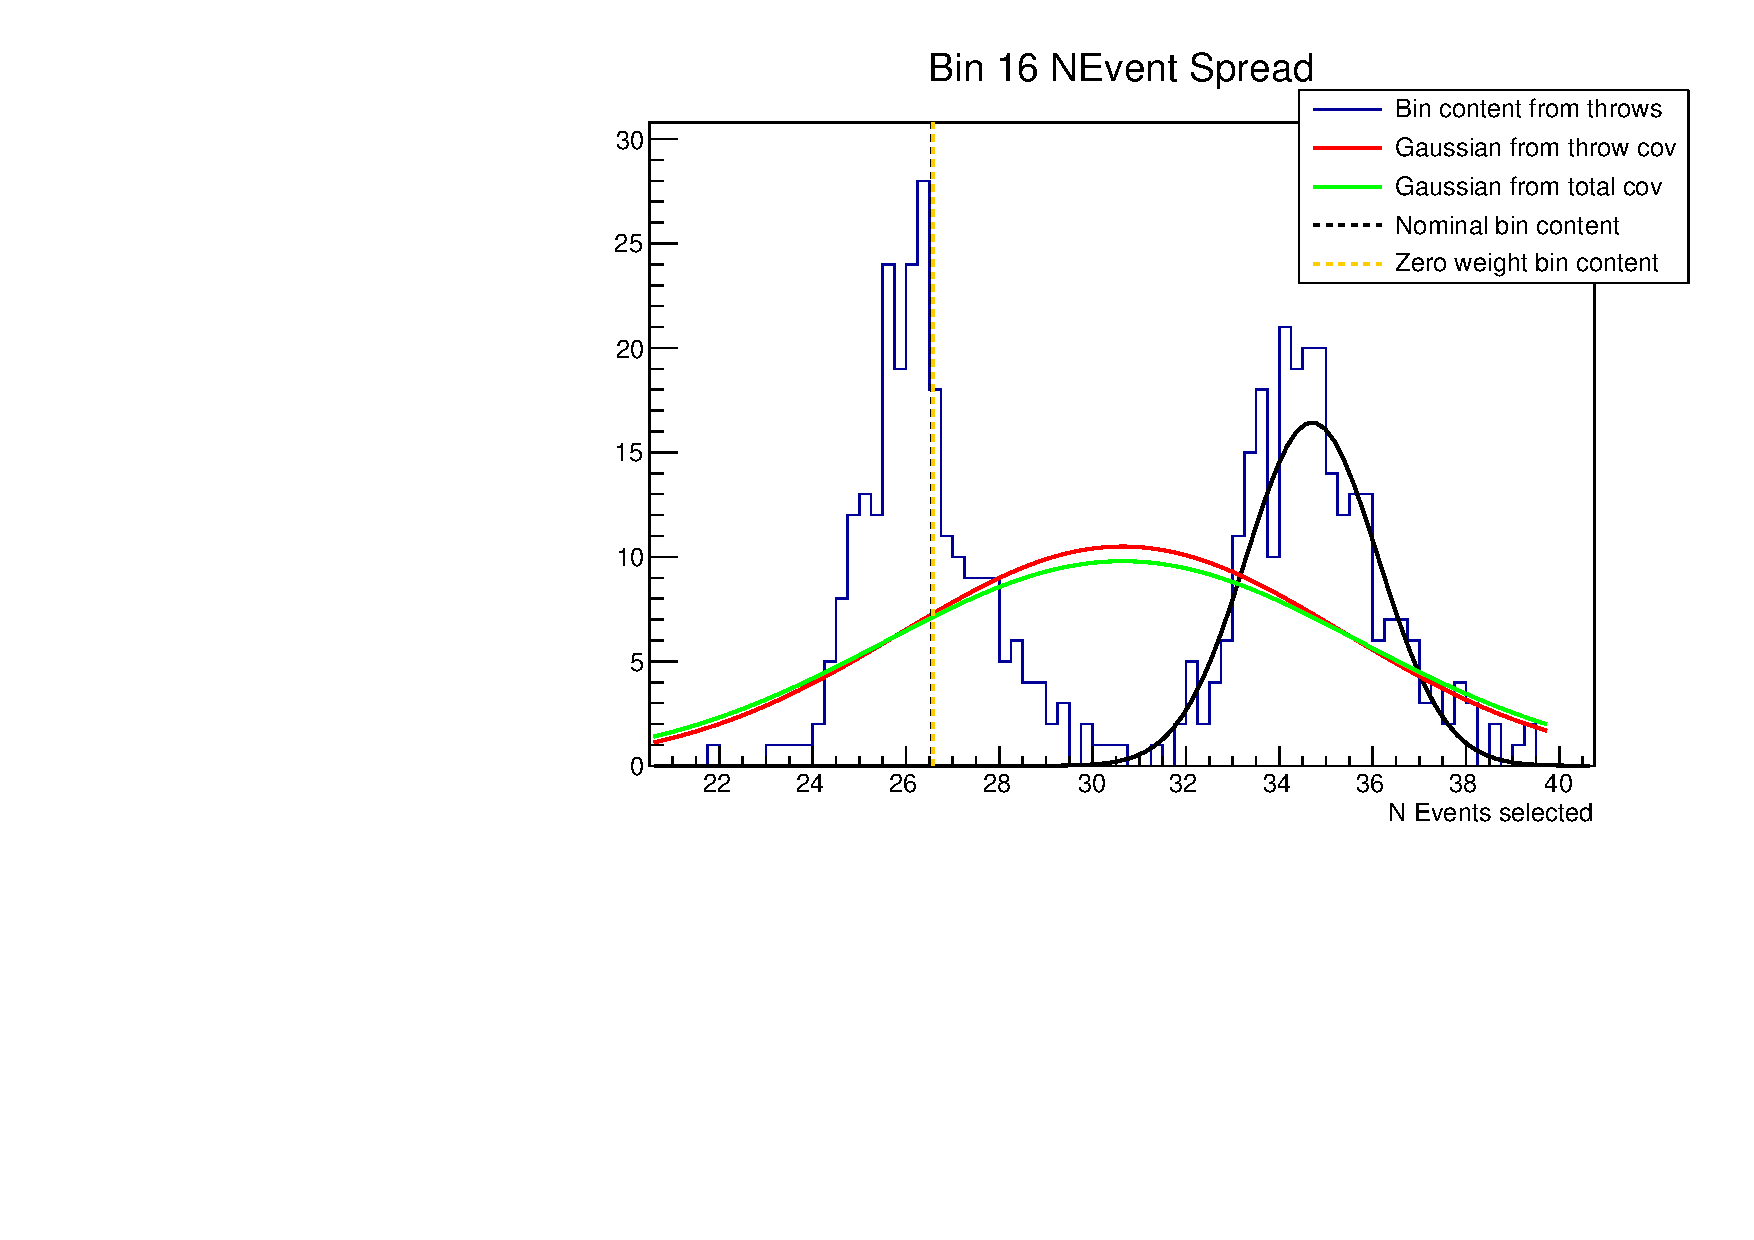
\includegraphics[width=\textwidth, trim={4mm 3mm 2mm 2mm}, clip,page=1]{figures/numu/syst/bad_bin}
		\caption{FGD1 CC0$\pi$, 1250-2000, 0.6-0.7}
	\end{subfigure}
	\begin{subfigure}[t]{0.42\textwidth}
		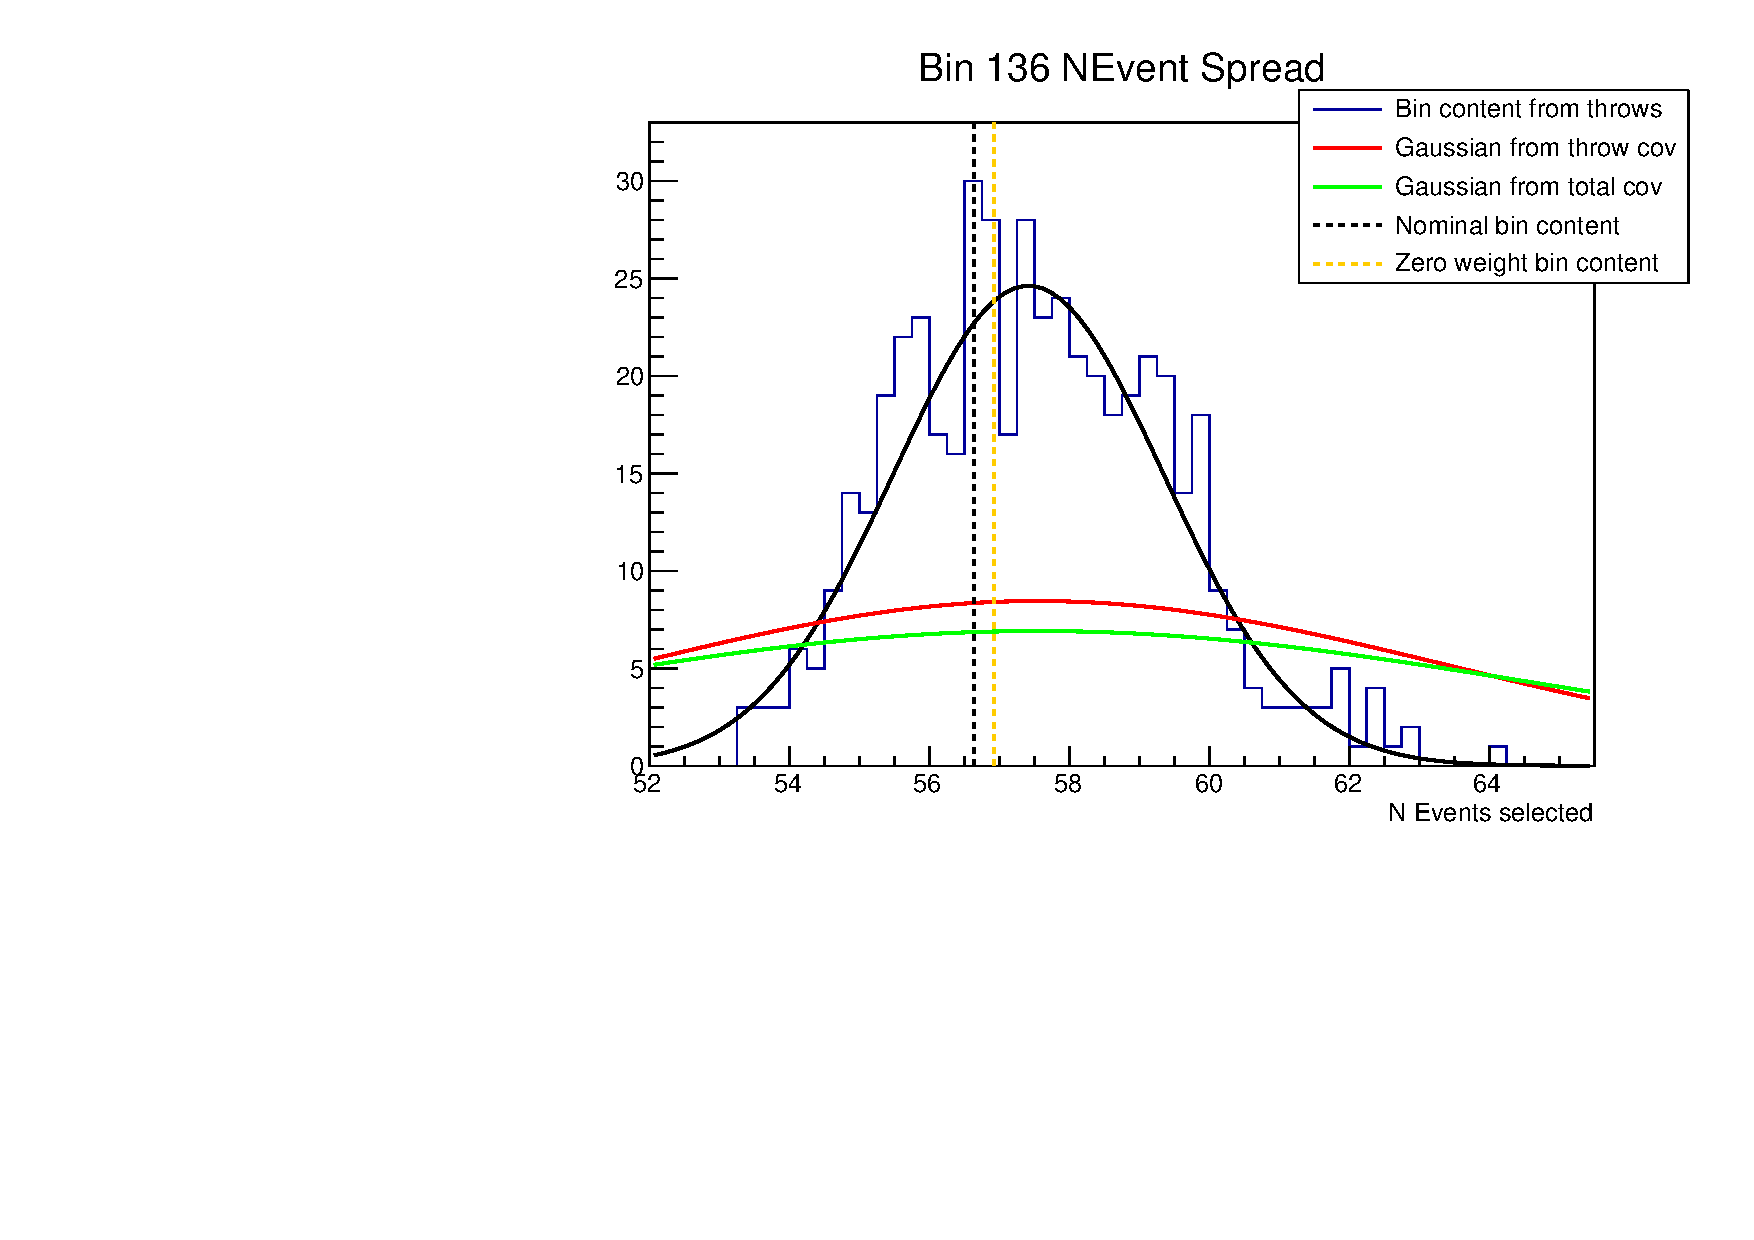
\includegraphics[width=\textwidth, trim={4mm 3mm 2mm 2mm}, clip,page=1]{figures/numu/syst/decent_bin}
		\caption{FGD1 CC1Trk, 0-400, 0.97-0.98}
	\end{subfigure}

	\begin{subfigure}[t]{0.42\textwidth}
		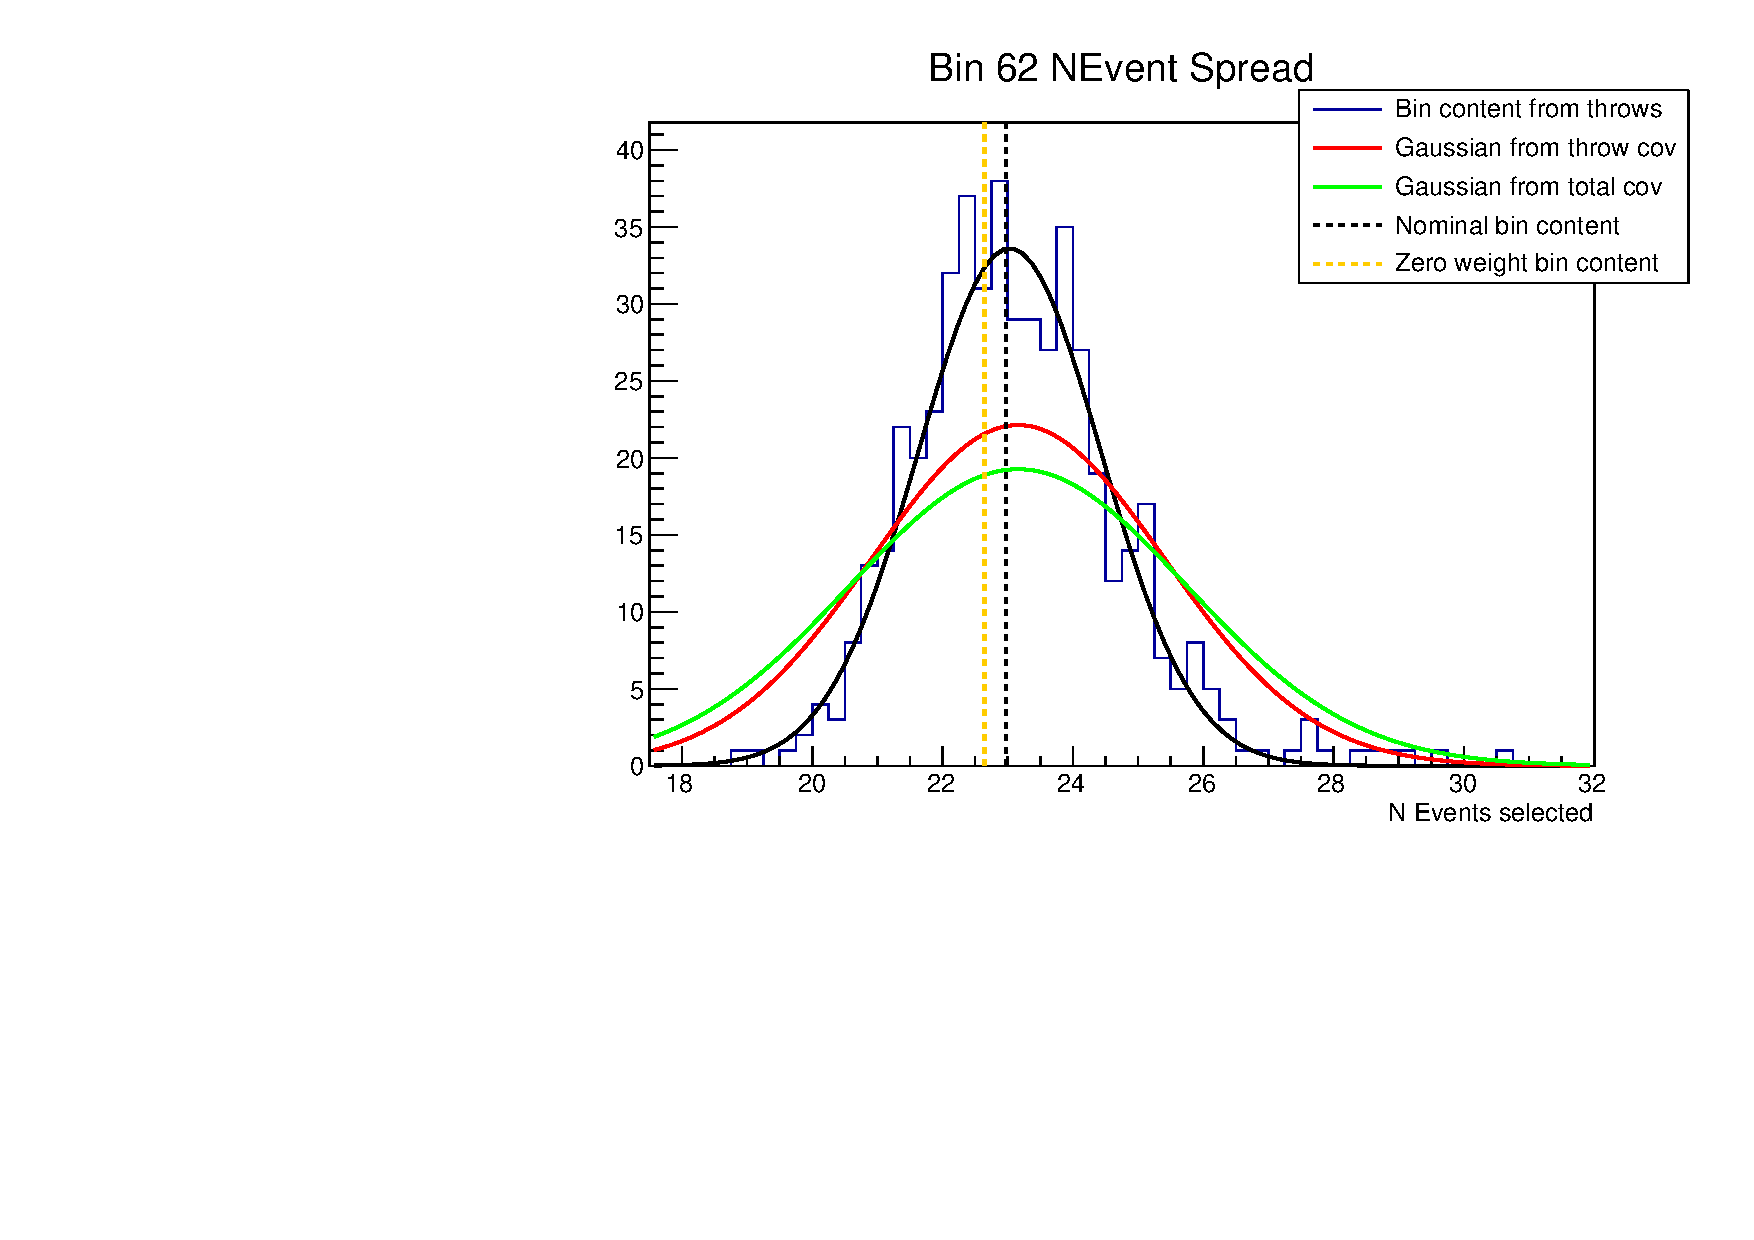
\includegraphics[width=\textwidth, trim={4mm 3mm 2mm 2mm}, clip,page=1]{figures/numu/syst/good_bin}
		\caption{FGD1 CC1$\pi$, 300-1250, 0.9-0.92}
	\end{subfigure}
	\begin{subfigure}[t]{0.42\textwidth}
		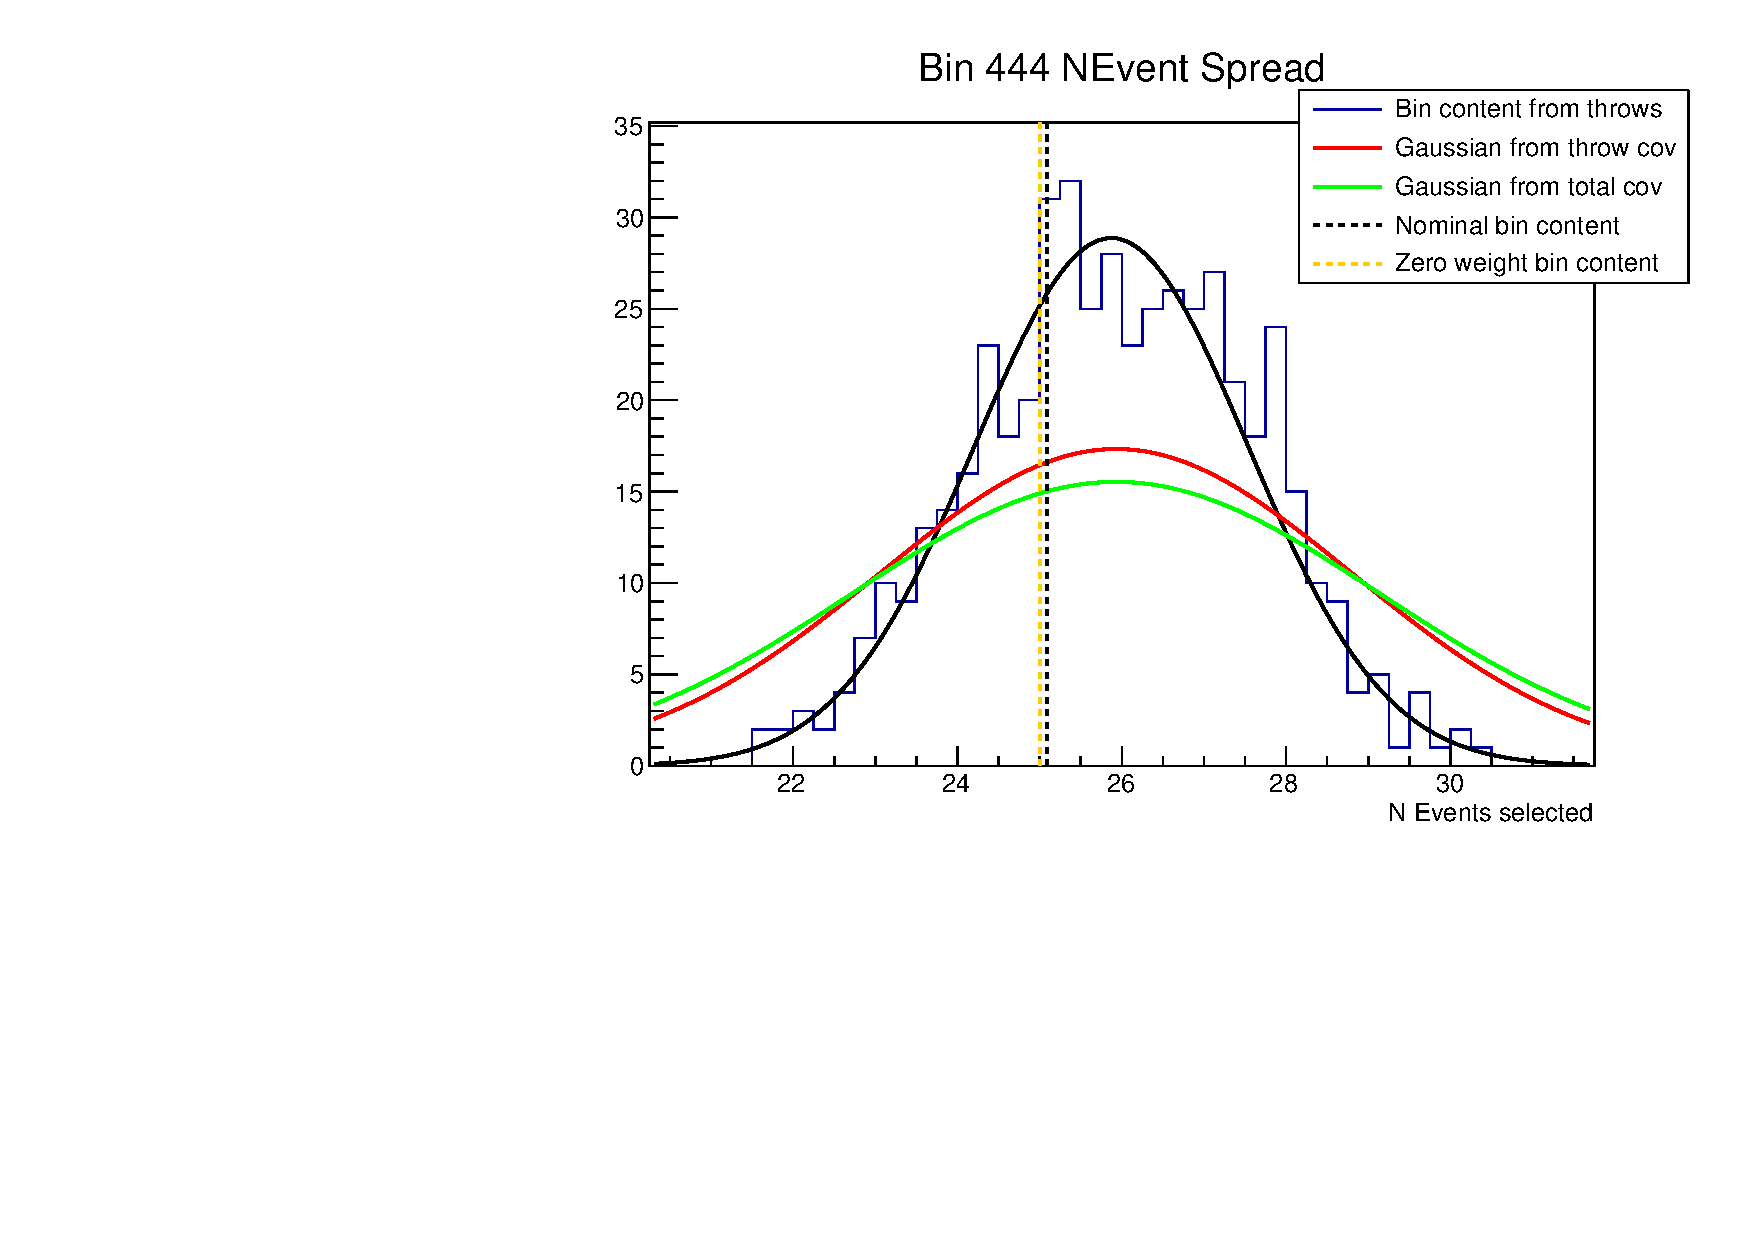
\includegraphics[width=\textwidth, trim={4mm 3mm 2mm 2mm}, clip,page=1]{figures/numu/syst/good_bin2}
		\caption{FGD2 CCNTrk, 0-700, 0.93-0.98}
	\end{subfigure}
	\caption{Number of events in selected detector bins with uncertainties from ND280 systematics}
	\label{fig:det_var}
\end{figure}
The result of the detector systematics procedure is shown in \autoref{fig:det_var} for a selection of bins. In FGD1 CC0$\pi$ we find the worst overall example in the \pmu=1250-2000, \cosmu=0.6-0.7 bin, in which we see a double Gaussian bimodal behaviour. This is likely from events migrating in and out of the \{\pmu, \cosmu, sample\} combination due to pion secondary interactions. Although a simple fit to the bin content chooses one of the peaks, the covariance matrix entry sits in between the two with an error that covers both modes.

The final covariance matrix is seen in \autoref{fig:nd280_cov}, where the majority of bins are highly correlated. The correlation matrix is shown in \autoref{fig:nd280_corr}. We particularly see high correlations for the high-momentum bins (towards the end of each selection). The anti-correlations enter mostly for RHC selections, where bins at low \pmu correlate negatively with bins at high \pmu. There are also anti-correlations in FGD1 vs FGD2 selections.
\begin{figure}[h]
	\begin{subfigure}[t]{0.70\textwidth}
		\includegraphics[width=\textwidth, trim={0mm 0mm 0mm 0mm}, clip,page=1]{figures/numu/syst/nd280_syst_cov.pdf}
	\end{subfigure}
\caption{$\text{sgn(}V_{i,j}\text{)}\times\sqrt{V_{i,j}}$ for the ND280 systematic parameters}
\label{fig:nd280_cov}
\end{figure}
\begin{figure}[h]
	\begin{subfigure}[t]{0.70\textwidth}
		\includegraphics[width=\textwidth, trim={0mm 0mm 0mm 0mm}, clip,page=2]{figures/numu/syst/nd280_syst_cov.pdf}
	\end{subfigure}
\caption{Correlation matrix for the ND280 systematic parameters}
\label{fig:nd280_corr}
\end{figure}

% Table with interaction parameters
%\begin{table}
%	\centering
%	\begin{tabular}{ l | c | c }
%		\hline
%		Parameter & Fit binning & Similar syst. merge \\
%		\hline
%		\hline
%		FSI INEL LO & $0.0 \pm 0.202$ & $0.0\pm0.200$ \\
%		FSI INEL HI & $0.0 \pm 0.235$ & $0.0\pm0.233$ \\
%		FSI PI PROD & $0.0 \pm 0.347$ & $0.0\pm0.344$ \\
%		FSI CEX LO  & $0.0 \pm 0.416$ & $0.0\pm0.412$ \\
%		FSI CEX HI  & $0.0 \pm 0.193$ & $0.0\pm0.191$ \\
%		$M_A^{QE}$  & $1.2 \pm 0.0517$ & $1.2\pm0.0512$ \\
%		$p_F^{C}$   & $217 \pm 36.96$ & $217\pm36.021$ \\
%		2p2h norm C & $100 \pm 30.79$ & $100\pm30.56$ \\
%		$E_B^{C}$   & $25.0 \pm 8.57$ & $25.0\pm8.56$ \\
%		$p_F^{O}$   & $225 \pm 57.61$  & $225\pm56.16$ \\
%		2p2h norm O & $100 \pm 277.98$ & $0.0\pm272.62$ \\
%		$E_B^{C}$   & $27.0 \pm 9.00$ & $27.0\pm9.00$ \\
%		$C_5^A$		& $1.01 \pm 0.066$ & $1.01\pm0.064$ \\
%		$M_A^{1\pi}$ & $0.95 \pm 0.060$ & $0.95\pm0.059$ \\
%		$I_{1/2}$ non-res & $1.30 \pm 0.180$ & $1.30\pm0.180$ \\
%		CC $\nu_e$ norm & $1.00 \pm 0.030$ & $1.00\pm0.030$ \\
%		DIS Shape	& $0.00 \pm 0.208$ & $0.0\pm0.208$ \\
%		CC Coherent norm & $1.0 \pm 0.258$ & $1.0\pm0.257$ \\
%		NC Coherent norm & $1.0 \pm 0.299$ & $1.0\pm0.299$ \\
%		NC Other & $1.0 \pm 0.182$ & $1.0\pm0.181$ \\
%		2p2h $\bar{\nu}$ & $1.0 \pm 0.332$ & $1.0\pm0.329$ \\
%		\hline
%	\end{tabular}
%	\caption{Cross-section parameter results from comparisons using fit binning and a merged binning for the 2015 cross-section model.}
%\label{fig:2017_rebin_asimov}
%\end{table}

\subsection{Cross-section}
\label{subsec:syst_xsec}
The parameterisation of the interaction systematics is frequently updated in T2K analyses to account for new theoretical calculations. This includes nuclear in-medium effects such as RPA and 2p2h corrections\cite{nieves1,nieves2}, initial state models such as Local Fermi Gases \cite{lfg} and Spectral Functions \cite{benhar}, and parameter tunes of existing models\cite{ccqe_tuning}.

The T2K and Super-K experiments both use the custom interaction library NEUT 5.3.3\cite{neut} as a primary generator, with cross-checks with GENIE\cite{genie} and NuWro\cite{NuWro}. Hence the interaction parameterisation deals with the models implemented into NEUT and are outlined here. The total cross-sections in $E_\nu$, $\sigma(E_\nu)$, for NEUT 5.3.3 are shown in \autoref{fig:neut_xsecs}

\begin{figure}[h]
	\centering
	\begin{subfigure}[t]{0.42\textwidth}
		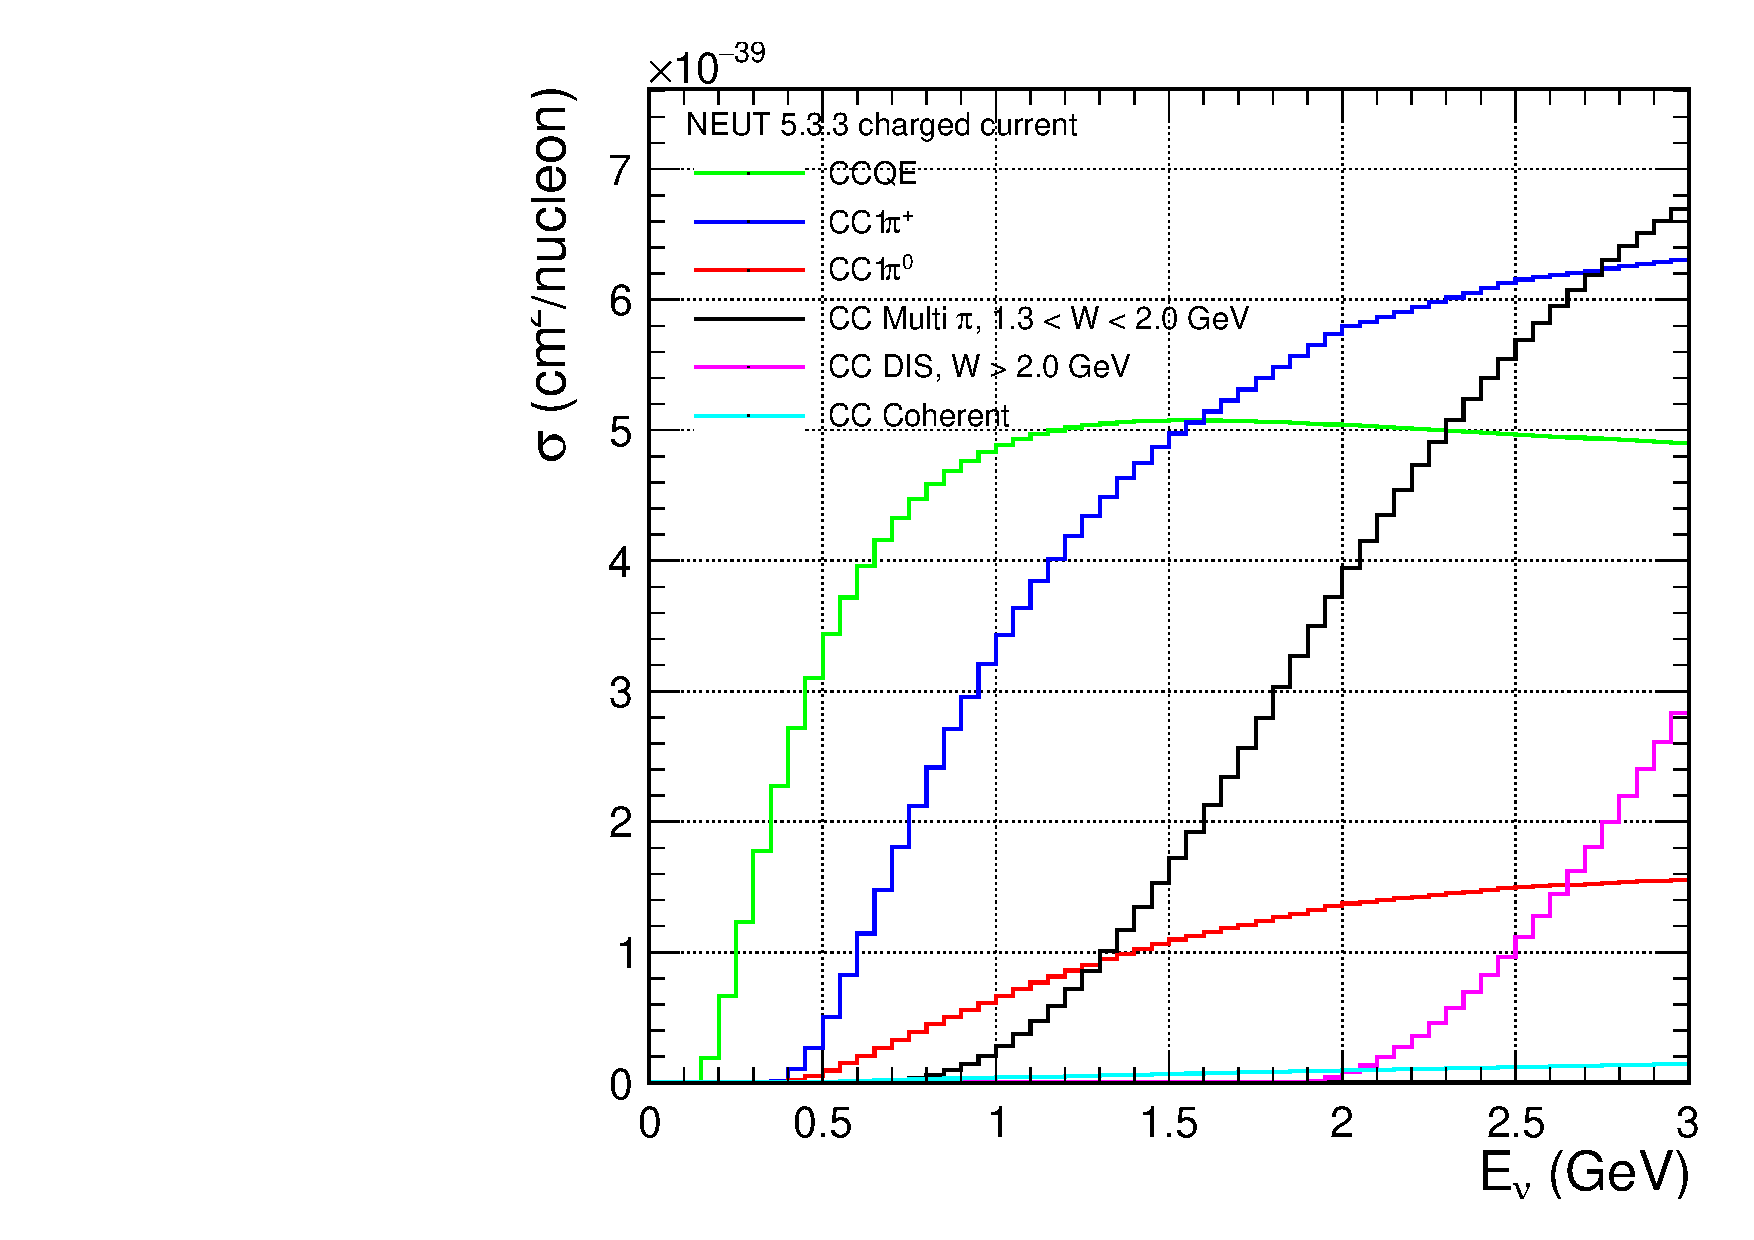
\includegraphics[width=\textwidth, trim={0mm 0mm 0mm 0mm}, clip,page=1]{figures/niwg/NEUT_533_xsecs}
		\caption{Charged current}
	\end{subfigure}
	\begin{subfigure}[t]{0.42\textwidth}
		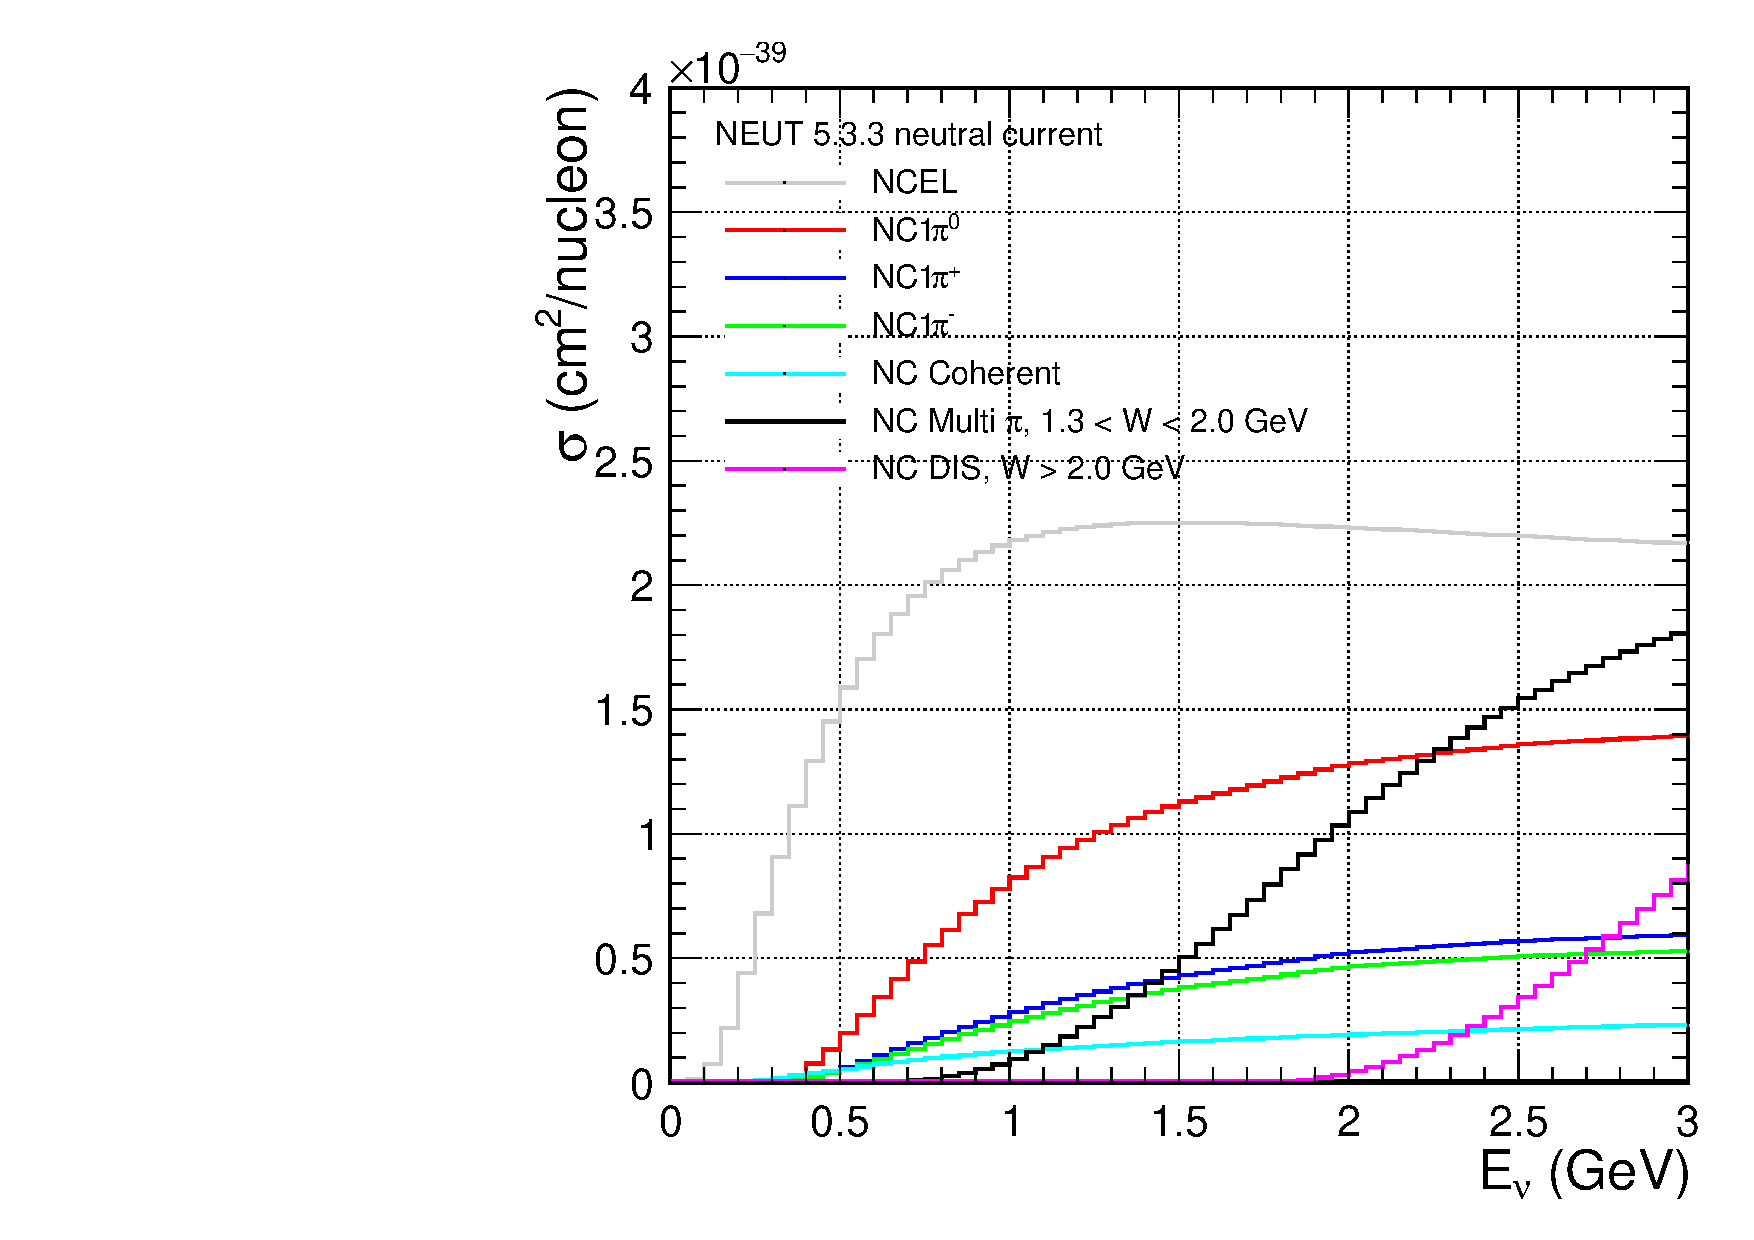
\includegraphics[width=\textwidth, trim={0mm 0mm 0mm 0mm}, clip,page=1]{figures/niwg/NEUT_533_xsecs_NC}
		\caption{Neutral current}
	\end{subfigure}
	\caption{Total cross-sections from the NEUT 5.3.3\cite{neut} neutrino interaction generator}
	\label{fig:neut_xsecs}
\end{figure}

\autoref{fig:neut_xsecs} shows at T2K energies ($E_\nu\sim0.6\text{ GeV}$) the primary interaction mode is CCQE. Charged pion production becomes important at $E_\nu\sim1\text{ GeV}$, and multi-$\pi$ and DIS above $E_\nu\sim2.5\text{ GeV}$. Since this analysis aims to minimise systematics for oscillation analyses---which select the charged-current 0$\pi$ final state at SK---the 0$\pi$ systematics have the largest impact. Single pion production make up $15-20\%$ of the 0$\pi$ selection by missing pions in either reconstruction or losing them to pion final state interactions before the pion exits the nucleus.

\red{talk about the factorisation into initial state, nucleon interaction, final state interaction}

\paragraph{CCQE and CC0$\pi$}
The nominal model is generated with a Spectral Function from Benhar et al (SF) \cite{benhar} and a 2-particle-2-hole (2p2h) excitation \cite{nieves1,nieves2} for the CCQE/CC0$\pi$ model. An alternative model uses the Llewellyn-Smith model\cite{llewelyn-smith} with a dipole axial form factor and BBBA05 vector form factors \cite{bbba05} with a Smith-Moniz Relativistic Fermi Gas (RFG) \cite{Smith-Moniz}. 

\autoref{fig:cc0pi_diag} shows some pseudo diagrams of the definition of the 0$\pi$, CCQE and one 2p2h process. The CC0$\pi$ signal definition does not include hadronic information, so the CCQE and 2p2h processes produce identical 0$\pi$ final states. Using CCQE energy reconstruction for 2p2h events would clearly bias $E_\nu$---as would be missing a pion in a single pion event due to thresholds or pion final state interaction.
\begin{figure}[h]
	\centering
	\begin{subfigure}[t]{0.32\textwidth}
		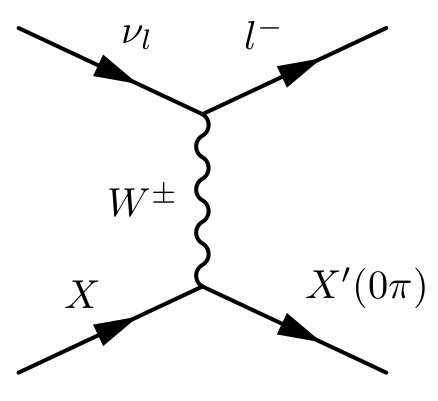
\includegraphics[width=\textwidth, trim={0mm 0mm 0mm 0mm}, clip,page=1]{figures/niwg/diagrams/CC0pi}
		\caption{CC0$\pi$}
	\end{subfigure}
	\begin{subfigure}[t]{0.32\textwidth}
		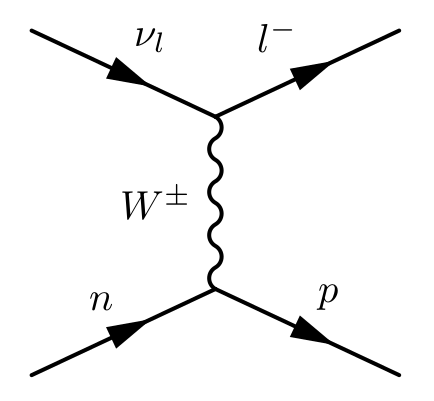
\includegraphics[width=\textwidth, trim={0mm 0mm 0mm 0mm}, clip,page=1]{figures/niwg/diagrams/CCQE}
		\caption{CCQE}
	\end{subfigure}
	\begin{subfigure}[t]{0.32\textwidth}
		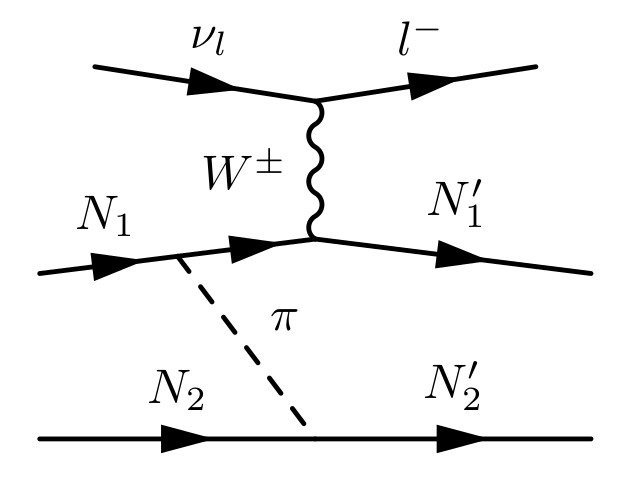
\includegraphics[width=\textwidth, trim={0mm 0mm 0mm 0mm}, clip,page=1]{figures/niwg/diagrams/2p2h_possibly}
		\caption{A 2p2h process}
	\end{subfigure}
	\caption{CC0$\pi$, CCQE and 2p2h pseudo-diagrams}
	\label{fig:cc0pi_diag}
\end{figure}

When selecting the default CCQE model for T2K analyses, it was found\cite{ccqe_tuning} that the SF+2p2h model was inferior to the RFG+2p2h+RPA when describing external neutrino and anti-neutrino CCQE scattering data from MiniBooNE\cite{miniboone_nu_ccqe, miniboone_nubar_ccqe} and MINER$\nu$A \cite{minerva_nu_ccqe, minerva_nubar_ccqe}. Thus the simpler RFG model was chosen and a one-time weight is applied in \pmu, \cosmu to account for the phase space shift.

In the selected CCQE model we have three free parameters to vary: $M_A^{QE}$, the axial mass in the dipole form factor parameterisation in the Llewelyn-Smith model, and $p_F$, the Fermi surface momentum, for $^{12}C$ and $^{16}O$ coming from the Smith-Moniz model\footnote{The binding energy term was found to have a negligible effect in 2015 analyses so was removed}.

The 2p2h effects first have normalisation parameters separated for neutrino and anti-neutrino, and one for $^{12}C\rightarrow^{16}O$ scaling. Secondly, there is a 2p2h shape parameter separated for $^{12}C$ and $^{16}O$ which is parameterised as a multiplicative weight applied on an event-by-event basis, taking an event's $E_\nu, q_0, q_3$, where $E_\nu$ is the true neutrino energy, $q_0$ is the energy and $q_3$ is the momentum components of $Q = k_\nu - k_\mu = (q_0, q_3)$. The 2p2h model can be parameterised as having terms with and without pion exchange and the interference between these terms. The parameterisation of the shape uncertainty is to at -1 assign all the 2p2h to $\Delta$-like or at +1 to non$\Delta$-like 2p2h, and an interference term soaking up the lost or gained cross-section so the systematic have no net effect on the normalisation of 2p2h events.

The net effect of the parameter on NEUT Monte-Carlo events generated with an ND280 flux on a $^{12}C$ target in $q_0, q_3$ (integrated over ND280 $E_\nu$) is shown in \autoref{fig:2p2h_shape_q0q3}. The $\sim300\text{ MeV}$ shift in $q_0$ from $m_\Delta-m_N$ is evident for the extreme parameter values, whereas the nominal (``Tweak Value = 0'') populates both regions.
\begin{figure}[h]
	\centering
	\begin{subfigure}[t]{0.32\textwidth}
		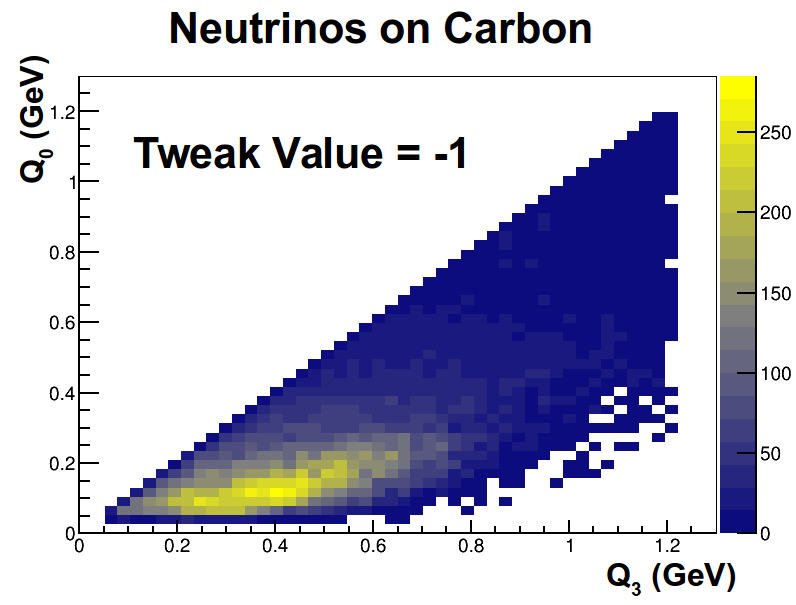
\includegraphics[width=\textwidth, trim={0mm 0mm 0mm 13mm}, clip,page=1]{figures/niwg/neutrino_carbon_m3}
	\end{subfigure}
	\begin{subfigure}[t]{0.32\textwidth}
		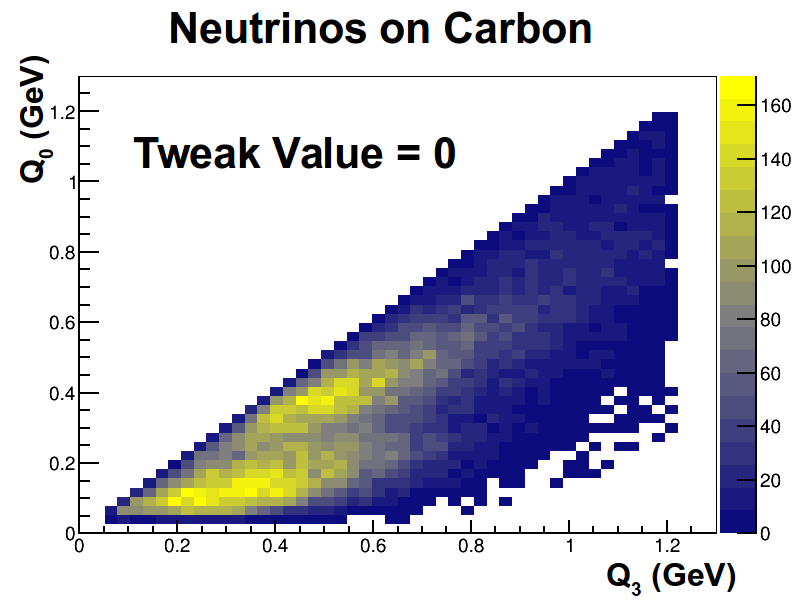
\includegraphics[width=\textwidth, trim={0mm 0mm 0mm 13mm}, clip,page=1]{figures/niwg/neutrino_carbon_0}
	\end{subfigure}
	\begin{subfigure}[t]{0.32\textwidth}
		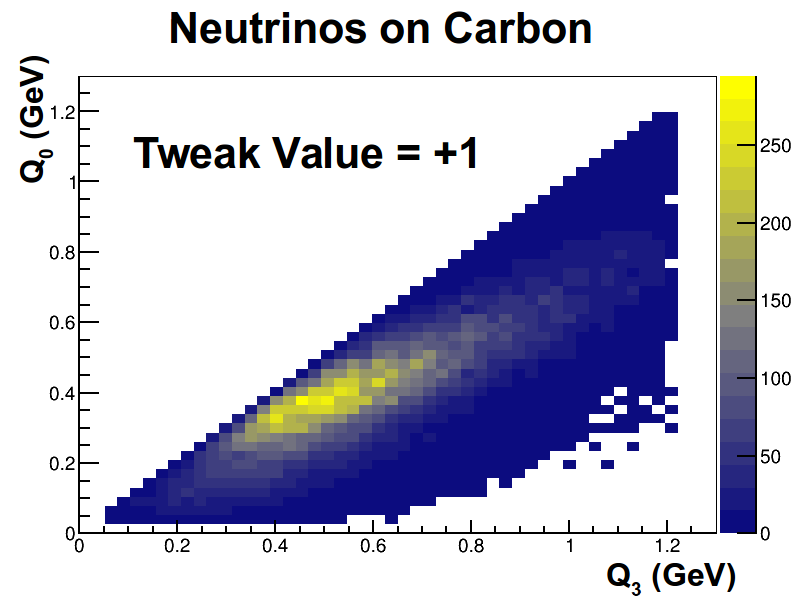
\includegraphics[width=\textwidth, trim={0mm 0mm 0mm 13mm}, clip,page=1]{figures/niwg/neutrino_carbon_p3}
	\end{subfigure}
\caption{$q_0,q3$ distributions for different values of the 2p2h shape parameter for $\nu_\mu$ on a $^{12}C$ target with the ND280 flux}
\label{fig:2p2h_shape_q0q3}
\end{figure}

\autoref{fig:2p2h_shape_enu} shows the $E_\nu^{reco}-E_\nu^{true}$ bias on the same generated events where the reconstructed neutrino energy is
\begin{equation}
	E_\nu^{reco} = \frac{m^2_f-m_i'^2-m^2_l+2m_i'E_l}{2(m_i'-E_l+p_l\cos\theta_{\nu,l})}
\end{equation}
in which $m_f$ is the final state nucleon mass, $m_i' = m_i-E_b$ where $m_i$ is the initial state nucleon mass and $E_b$ is the binding energy of a nucleon in the nucleus (27 MeV for $^{16}O$, 25 MeV for $^{12}C$), $E_l$ ($p_l$) is the reconstructed lepton energy (momentum), and $\cos\theta_{\nu,l}$ is the cosine of the reconstructed angle between the incoming neutrino and outgoing lepton.
\begin{figure}[h]
	\centering
	\begin{subfigure}[t]{0.42\textwidth}
		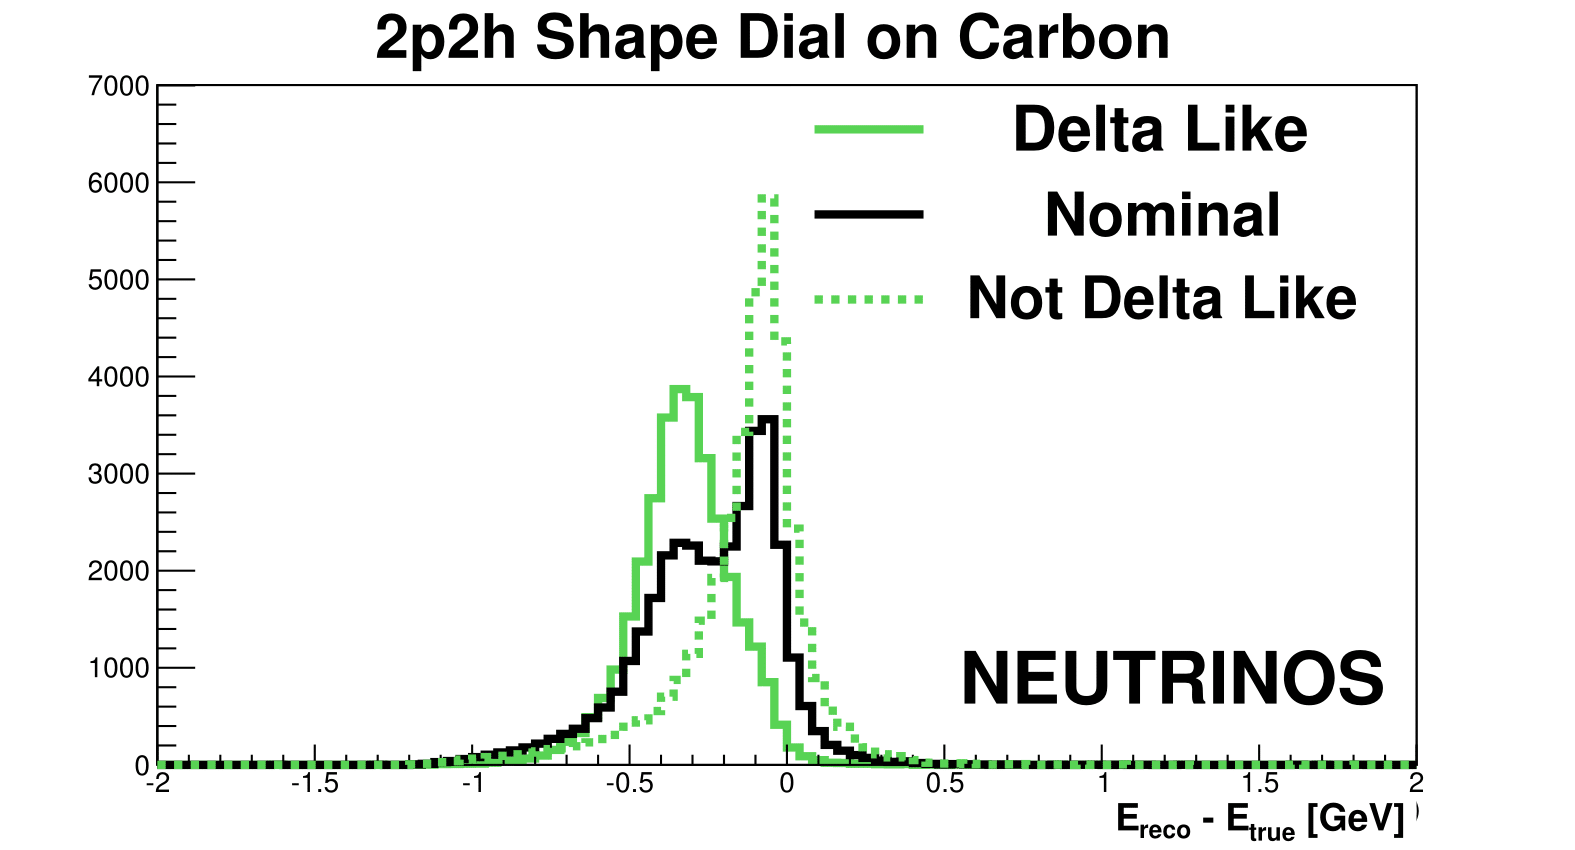
\includegraphics[width=\textwidth, trim={30mm 0mm 38mm 26mm}, clip,page=1]{figures/niwg/ediff_neutrino_mec_pdd_c}
		\caption{$^{12}C$ target}
	\end{subfigure}
	\begin{subfigure}[t]{0.42\textwidth}
		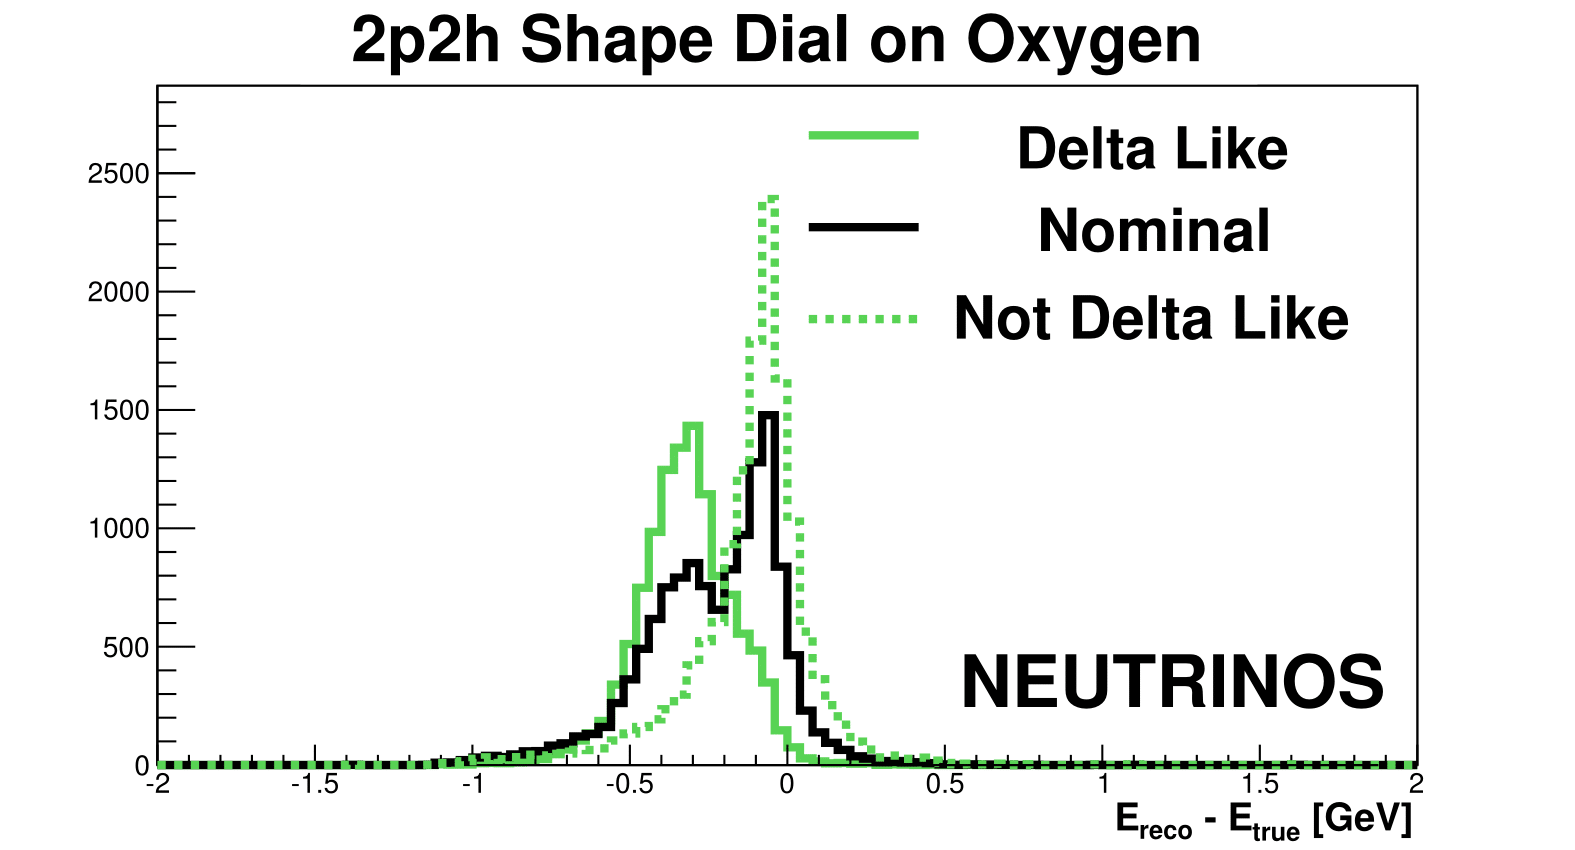
\includegraphics[width=\textwidth, trim={30mm 0mm 38mm 27mm}, clip,page=1]{figures/niwg/ediff_neutrino_mec_pdd_o}
		\caption{$^{16}O$ target}
	\end{subfigure}

\begin{subfigure}[t]{0.42\textwidth}
	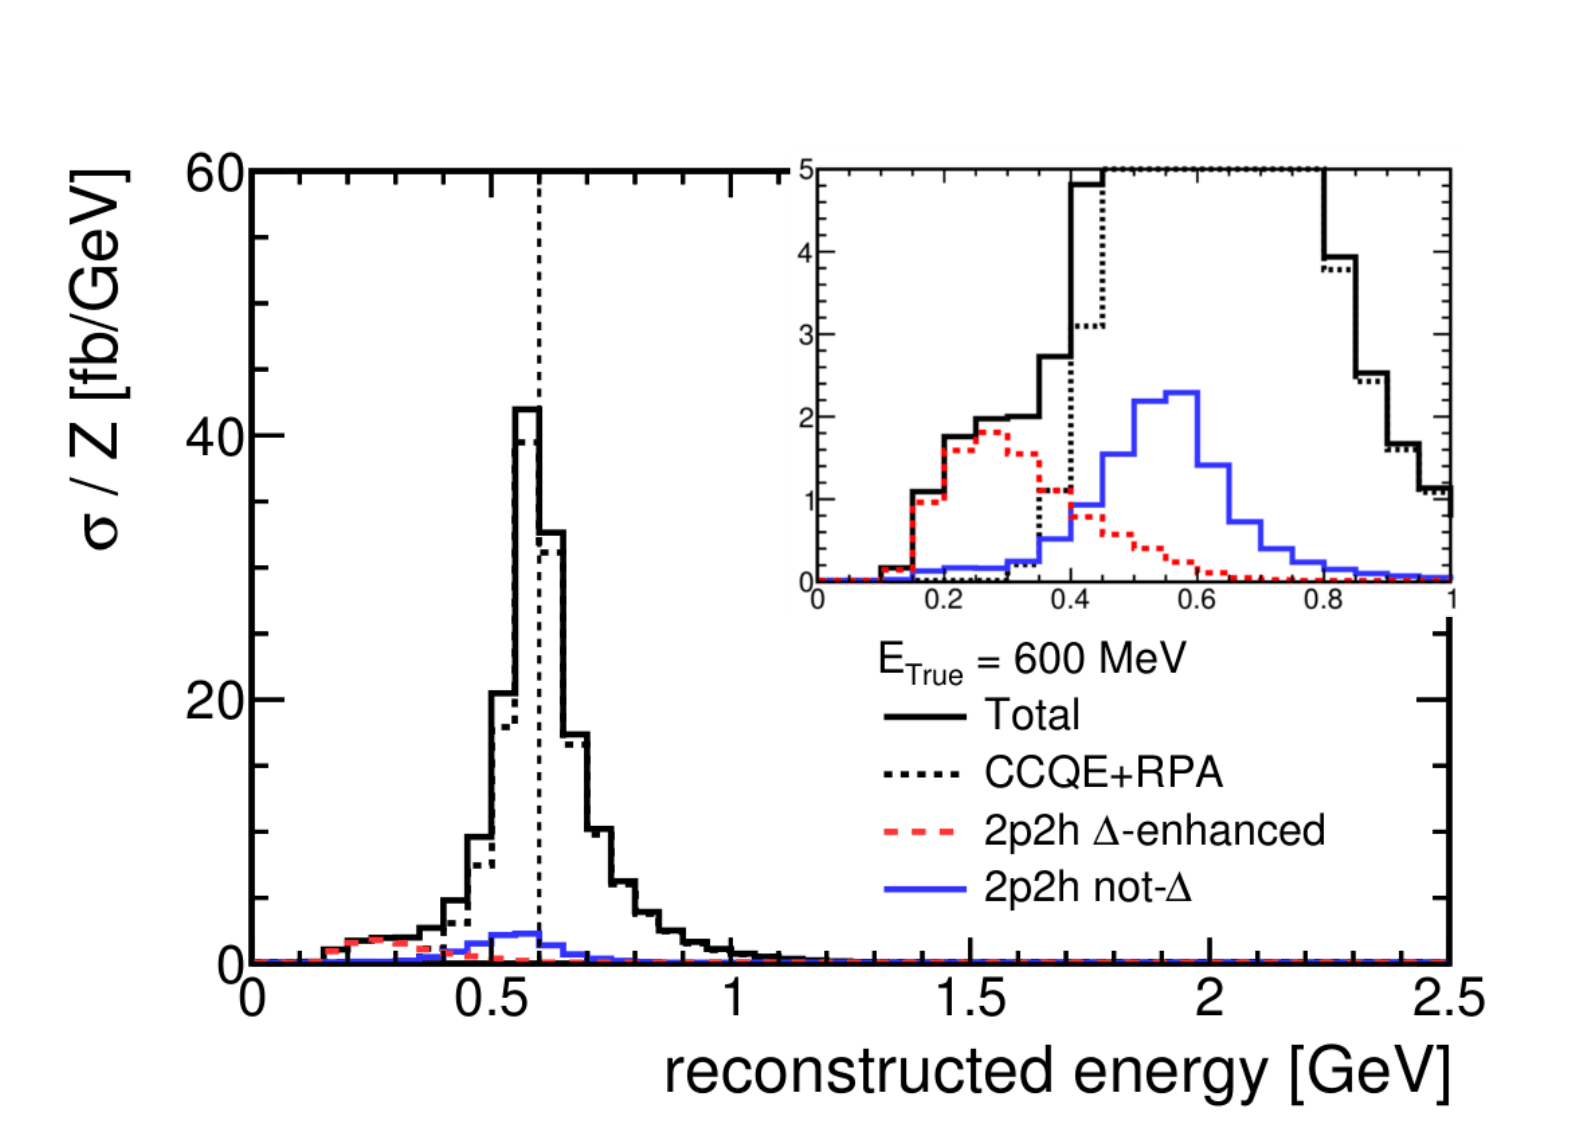
\includegraphics[width=\textwidth, trim={20mm 10mm 25mm 40mm}, clip,page=1]{figures/niwg/delta_notdelta}
	\caption{$E_\nu^{reco}$ for $E_\nu^{true}=0.6\text{ GeV}$ events on CH at ND280 for 0$\pi$ final states}
	\label{fig:2p2h_shape_enu_reco}
\end{subfigure}
	\caption{$E_\nu$ reconstruction bias for different values of the 2p2h shape parameter for $\nu_\mu$ with the ND280 flux in NEUT 5.3.3}
	\label{fig:2p2h_shape_enu}
\end{figure}

\autoref{fig:2p2h_shape_enu_reco} shows the importance of good 2p2h modelling for SK $E_\nu$ reconstruction: it biases 2p2h events towards a lower energy and so directly impact oscillation parameter fits.

The second class of uncertainties comes from the Random Phase Approximation \cite{nieves2}, which effectively describes correlations between nucleons in a nucleus. The net effect is to modify the 1-particle-1-hole\cite{nieves1} cross-section, which in NEUT is parameterised as a look-up table correction to the CCQE cross-section in $E_\nu$ and $Q^2$. The $E_\nu$ dependence was found to be relatively weak, so a $Q^2$ dependent correction was developed to mimic the uncertainties associated with the model\cite{nieves1}. The correction is parameterised as a third order rising polynomial which switches a decaying exponential at $Q^2=1.2\text{ GeV}^2$. A normal polynomial of form $ax^3+bx^2+cx+d$ connecting to $\exp{\left(-e(x-f)\right)}$ was found to strongly correlate the polynomial and exponential parameters, so a Bernstein polynomial base was chosen instead. The parameterisation follows

\begin{equation}
w(Q^2) = 
\begin{cases}
A(1-x')^{3} + 3B(1-x')^{2}x' + 3p_{1}(1-x')x'^{2} + Dx'^{3}, & x \le U \\
1 + p_{2}\exp(-E(x-U)), & x > U
\end{cases}
\end{equation}
in which $w(Q^2)$ is the weight from the RPA variation applied to CCQE events, $x=Q^2$, $x'=Q^2/U$, and $A, B, D$ and $E$ are normalisation factors for the four basis functions. Continuity between the functions at $Q^2=U$ is required and $p_1$ and $p_2$ absorb this if
\begin{equation}
	p_1= D+U\frac{E(D-1)}{3}, 
	p_2 = D-1
\end{equation}
The magnitude and uncertainty of $A, B, D$ and $E$ are then chosen to match the uncertainties provided in \cite{nieves2}. \autoref{fig:berpa_throws} shows the uncertainty bands from each parameter for the final values, showing how BeRPA A controls low $Q^2$, BeRPA B intermediate $Q^2$, BeRPA D medium $Q^2$ and BeRPA E high $Q^2$.
\begin{figure}[h]
	\centering
	\begin{subfigure}[t]{0.42\textwidth}
		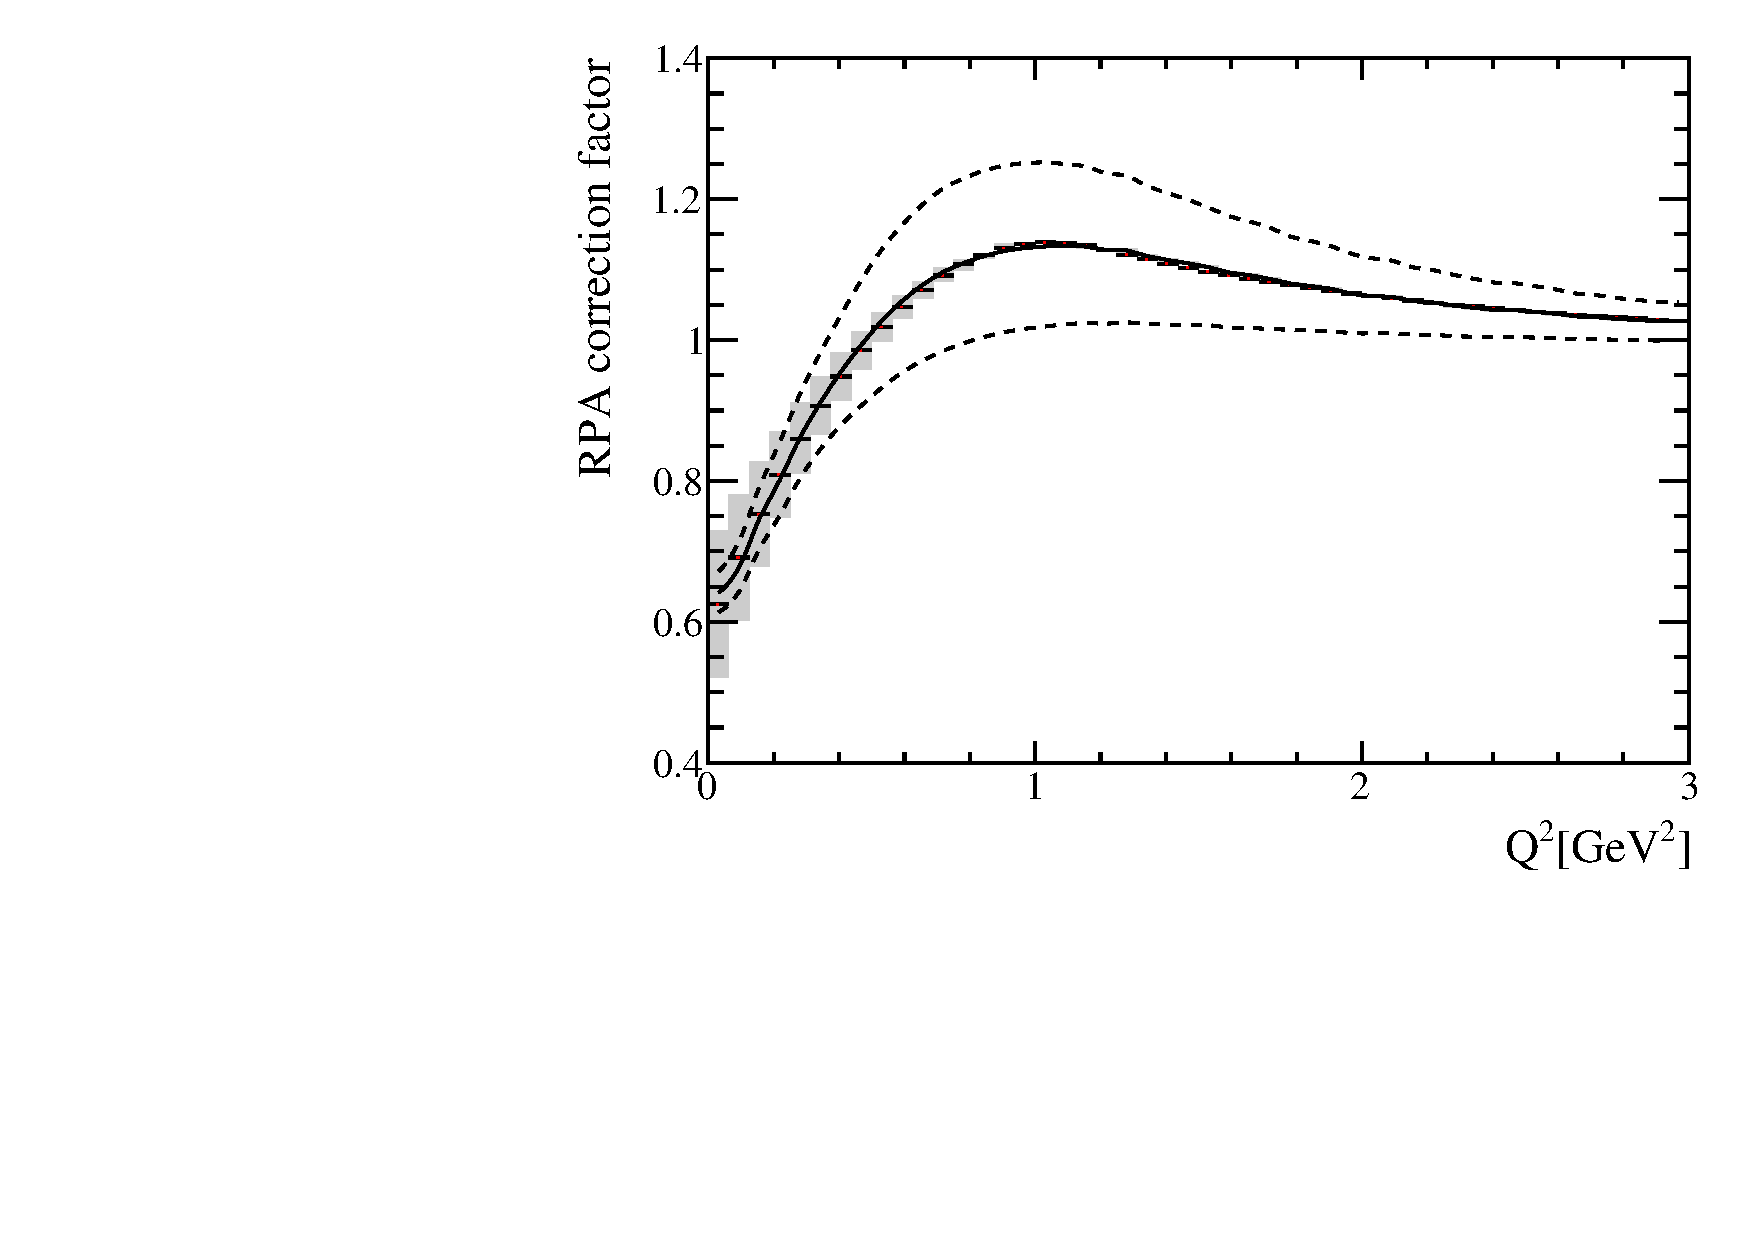
\includegraphics[width=\textwidth, trim={0mm 0mm 0mm 0mm}, clip,page=1]{figures/niwg/erpa_20percentA_throws}
		\caption{BeRPA A}
	\end{subfigure}
	\begin{subfigure}[t]{0.42\textwidth}
		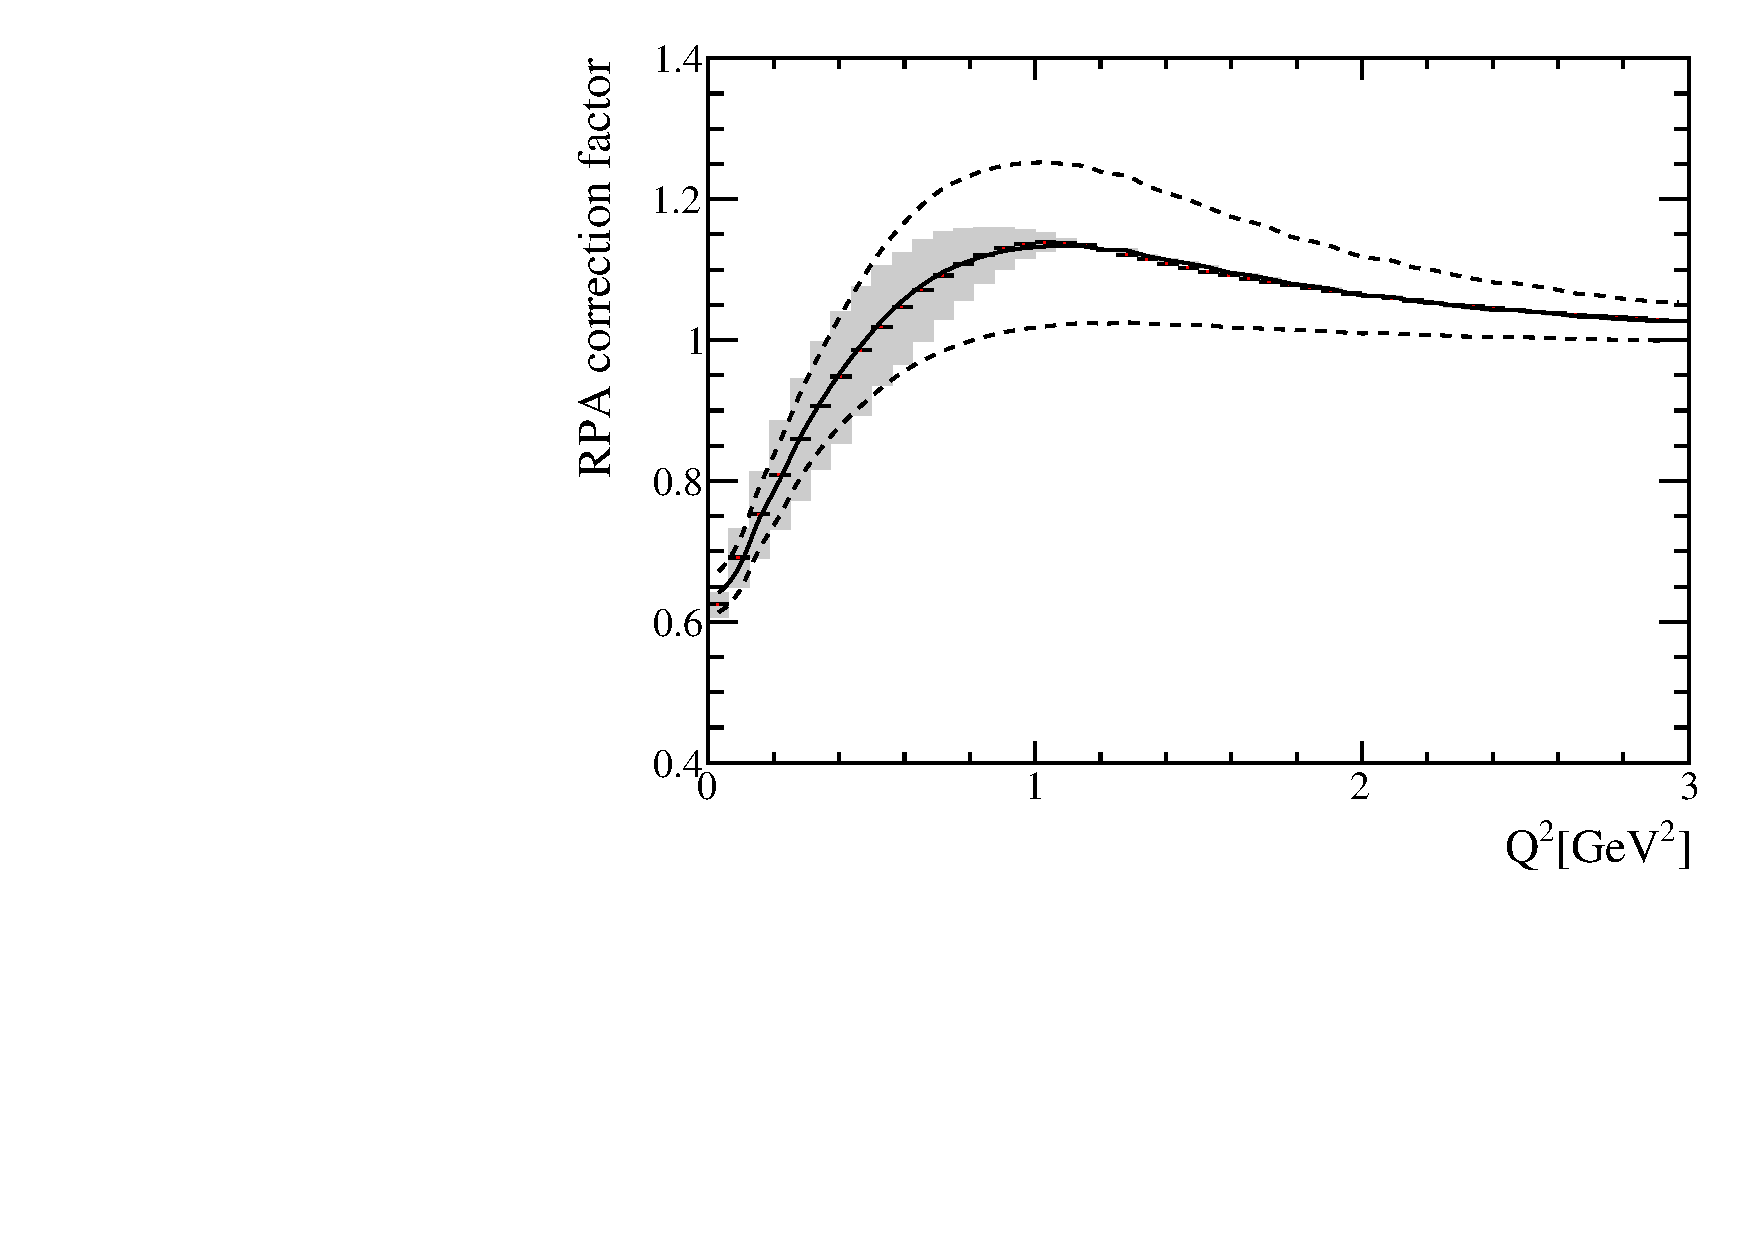
\includegraphics[width=\textwidth, trim={0mm 0mm 0mm 0mm}, clip,page=1]{figures/niwg/erpa_20percentB_throws}
		\caption{BeRPA B}
	\end{subfigure}

	\begin{subfigure}[t]{0.42\textwidth}
		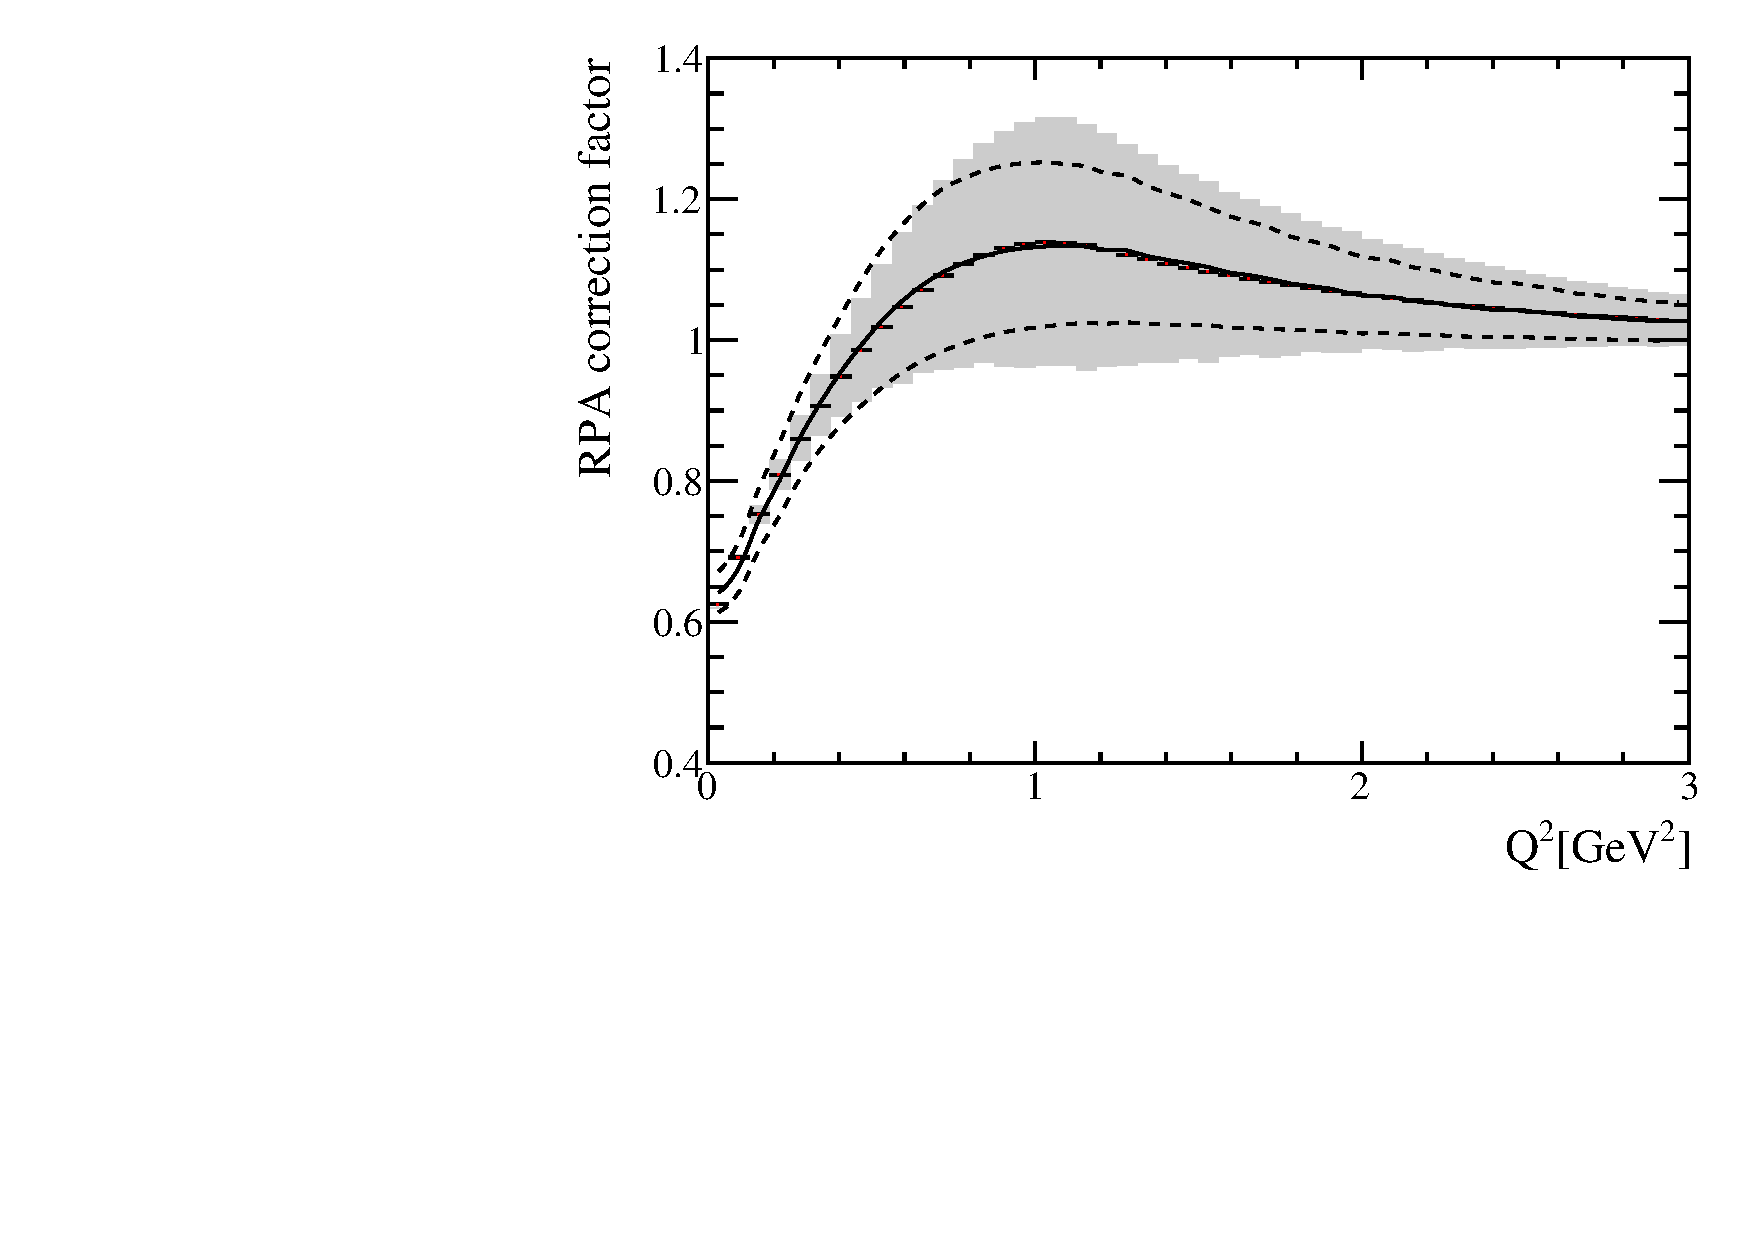
\includegraphics[width=\textwidth, trim={0mm 0mm 0mm 0mm}, clip,page=1]{figures/niwg/erpa_15percentD_throws}
		\caption{BeRPA D}
	\end{subfigure}
	\begin{subfigure}[t]{0.42\textwidth}
		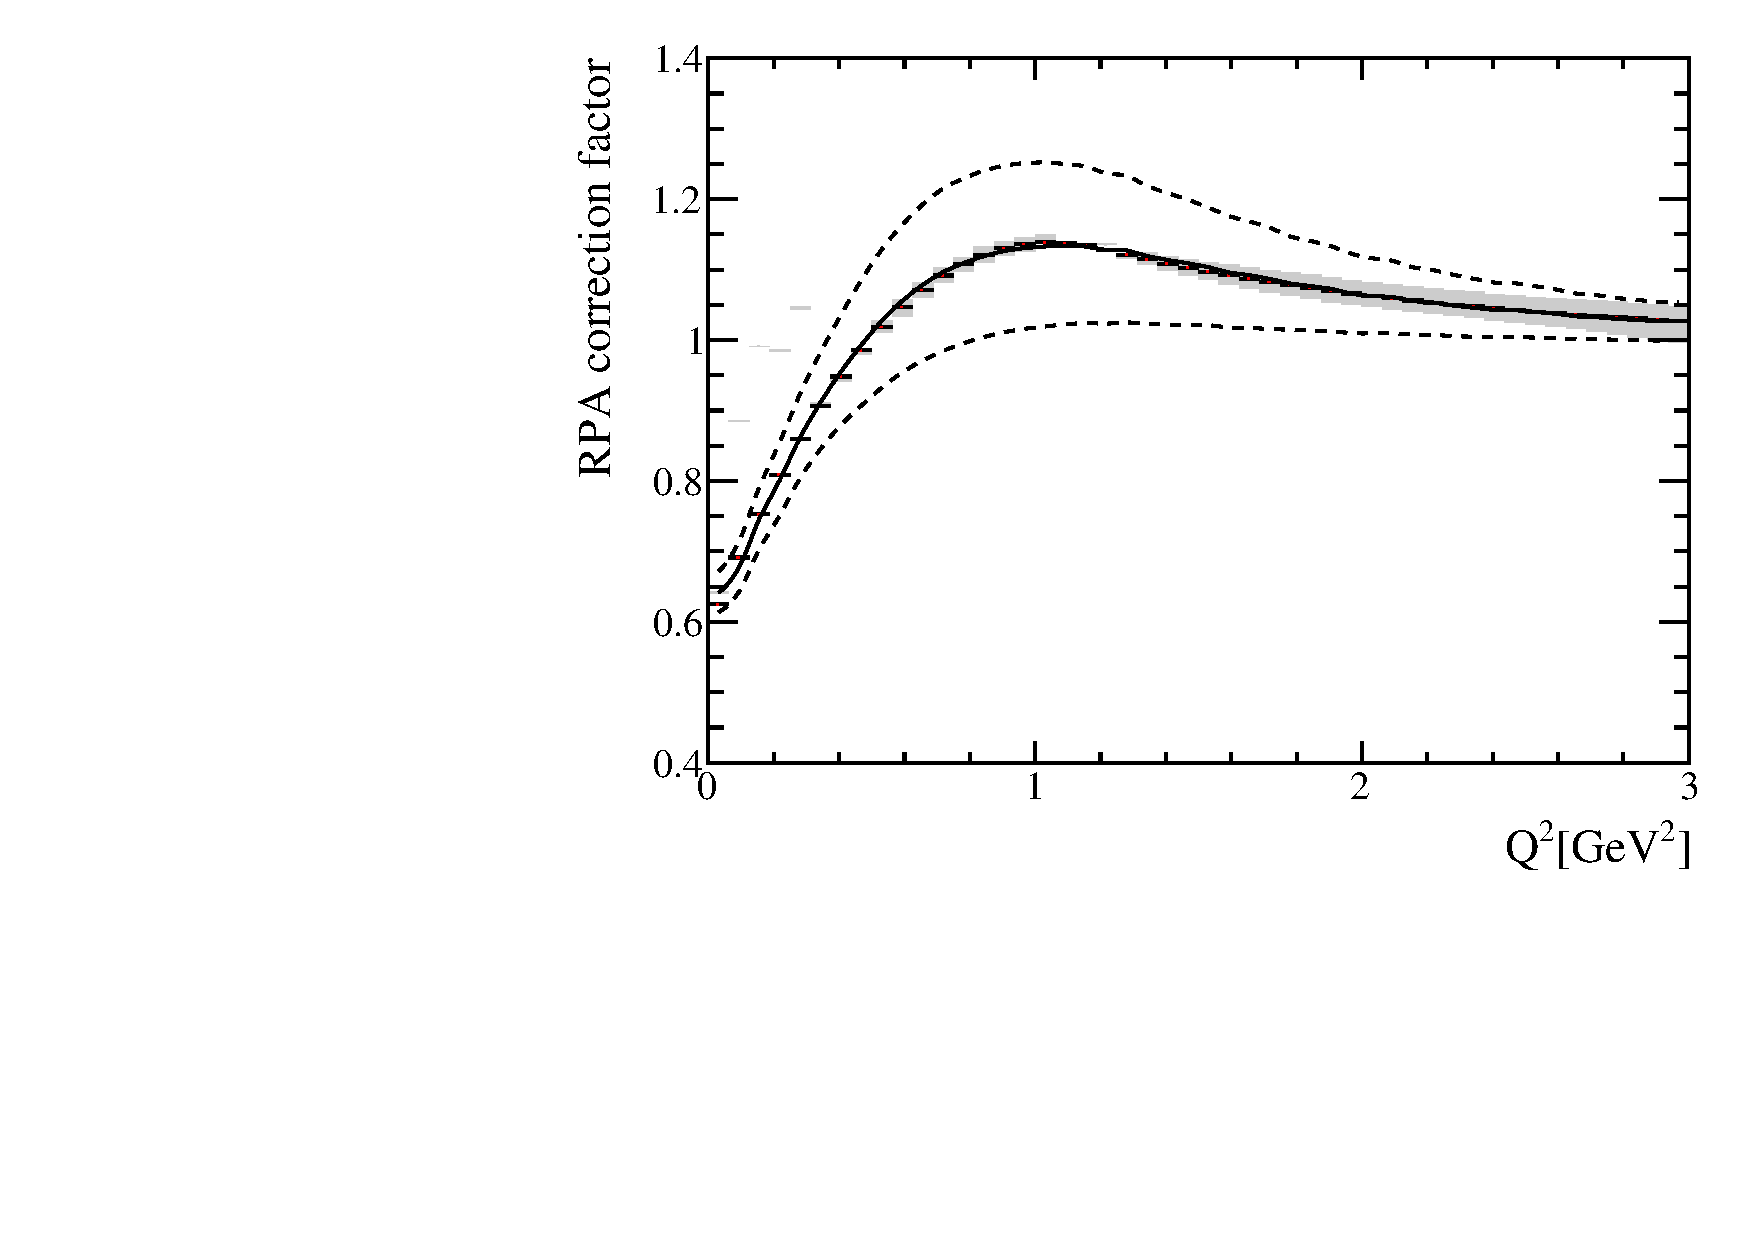
\includegraphics[width=\textwidth, trim={0mm 0mm 0mm 0mm}, clip,page=1]{figures/niwg/erpa_40percentE_throws}
		\caption{BeRPA E}
	\end{subfigure}
	\caption{BeRPA uncertainties for each separate parameter. The dashed line represents the theoretical uncertainties}
	\label{fig:berpa_throws}
\end{figure}

\paragraph{Single pion production}
The single pion production is described with the Rein-Sehgal model\cite{Rein_Sehgal, Rein_Angular} with lepton mass corrections \cite{Kuzmin_MassEffect,Wroclaw_MassEffect,Berger_Sehgal_MassEffect} and modified form factors aimed at the $\Delta$ resonance \cite{Wroclaw_CC1pi_2014,Wroclaw_CC1pi_2009,Wroclaw_CC1pi_theory}. The tunable parameters all relate to the neutrino-nucleon scattering interaction in the Rein-Sehgal model, which are $M_A^{RES}$, the axial mass for the resonant interaction in the Rein-Sehgal model, $C_5^A(0)$, one of the axial form factors at $Q^2=0$ in the Graczyk-Sobczyk form factor parameterisation, and the size of the non-resonant $I_{1/2}$ background in the Rein-Sehgal model.. 

\autoref{fig:1pi_diags} shows the charged-current neutrino-nucleon processes described by the model. The models also extend to anti-neutrino and neutral-current processes. In the case of missing a pion due to detector thresholds and/or pion interactions the neutrino energy is clearly biased by at least $E=m_\pi$.
\begin{figure}[h]
	\centering
	\begin{subfigure}[t]{0.32\textwidth}
		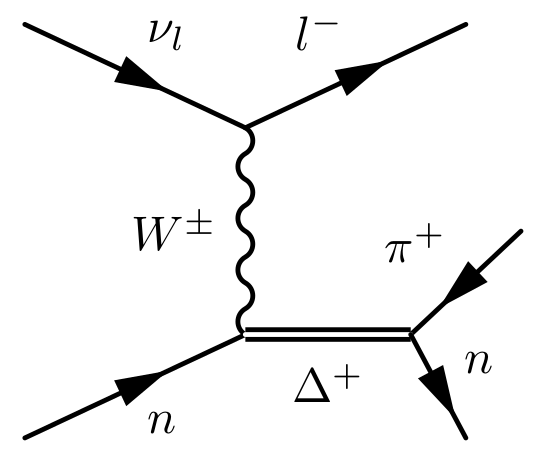
\includegraphics[width=\textwidth, trim={0mm 0mm 0mm 0mm}, clip,page=1]{figures/niwg/diagrams/CC1npip}
		\caption{CC1$\pi^+$1n}
	\end{subfigure}
	\begin{subfigure}[t]{0.32\textwidth}
		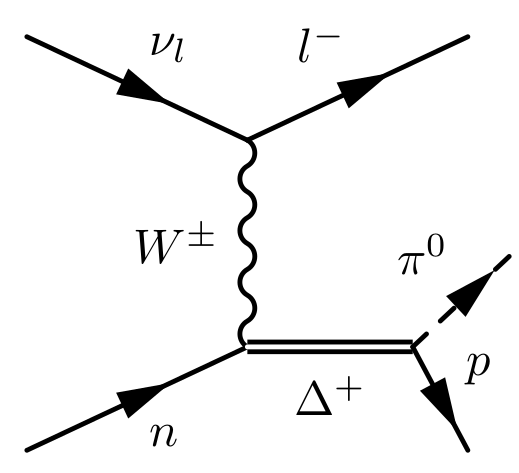
\includegraphics[width=\textwidth, trim={0mm 0mm 0mm 0mm}, clip,page=1]{figures/niwg/diagrams/CC1pi0}
		\caption{CC1$\pi^0$}
	\end{subfigure}
	\begin{subfigure}[t]{0.32\textwidth}
		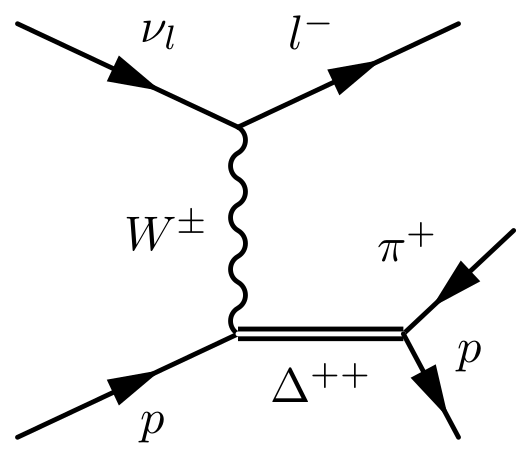
\includegraphics[width=\textwidth, trim={0mm 0mm 0mm 0mm}, clip,page=1]{figures/niwg/diagrams/CC1ppip}
		\caption{CC1$\pi^+$1p}
	\end{subfigure}
	\caption{Charged-current single pion production on a nucleon via a $\Delta$ resonances}
	\label{fig:1pi_diags}
\end{figure}

The single pion production uncertainties were tuned to selected bubble chamber data from ANL\cite{ANL_CC1pi,ANL_NC1pi} and BNL\cite{BNL_CC1pi,BNL_CC1pi_isospin,BNL_NuInt02}. The parameter values were cross-checked with modern corrections\cite{ANL_BNL_corr} and nuclear data from MiniBooNE\cite{MB_CC1pip,MB_CC1pi0,MB_NC1pi0}, MINER$\nu$A\cite{MIN_CC1pi0,MIN_CC1pip,MIN_pion_2016} and K2K \cite{K2K_CC1pip} using NUISANCE\cite{NUISANCE}.

\paragraph{Coherent scattering}
The coherent scattering model is described by the Rein-Sehgal model \cite{Rein_Sehgal_coh}. This process has a small cross-section but occupies a very specific phase space region: the very forward going, collinear lepton-pion system, and low $Q^2$ region. Furthermore it shares final state with single pion production. The interaction diagram is shown in \autoref{fig:coh_diags}.
\begin{figure}[h]
	\centering
	\begin{subfigure}[t]{0.42\textwidth}
		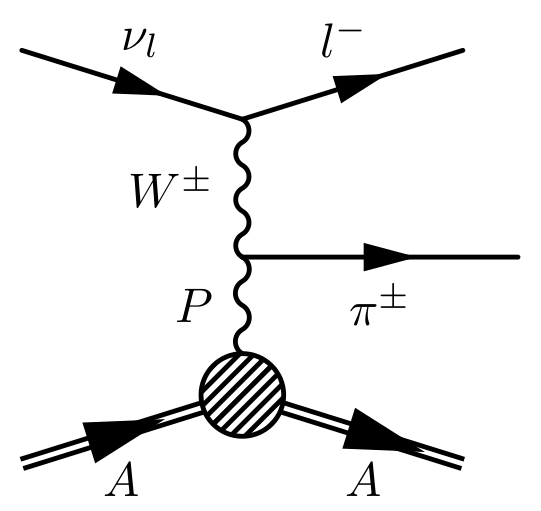
\includegraphics[width=\textwidth, trim={0mm 0mm 0mm 0mm}, clip,page=1]{figures/niwg/diagrams/CCcoh}
		\caption{CC coherent}
		\label{fig:coh_diags}
	\end{subfigure}
	\begin{subfigure}[t]{0.42\textwidth}
		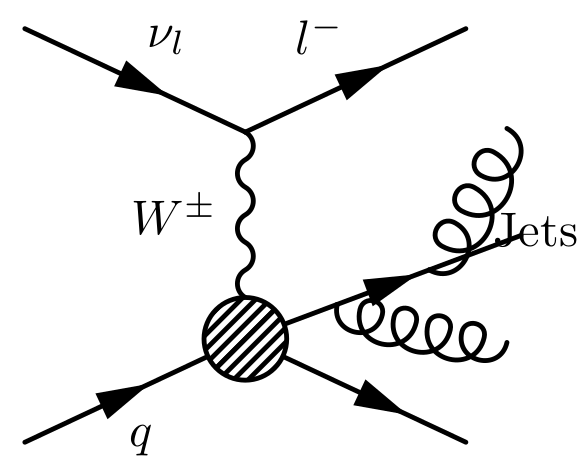
\includegraphics[width=\textwidth, trim={0mm 0mm 0mm 0mm}, clip,page=1]{figures/niwg/diagrams/CCmultipion}
		\caption{CC DIS}
		\label{fig:dis_diags}
	\end{subfigure}
	\caption{Coherent and multi-pion/DIS scattering diagrams}
	\label{fig:coh_dis_diags}
\end{figure}

An $E_\pi$ dependent scaling factor, listed in \autoref{tab:rein_sehgal_coh}, is applied to match MINER$\nu$A $\nu$ and $\bar{\nu}$ CC coherent data \cite{MIN_coh} and the Berger-Sehgal model \cite{Berger_Sehgal_coh}.
\begin{table}[h]
	\begin{tabular}{c | c}
		\hline
		\hline
		$E_\pi$ & Weight \\
		\hline
		0.00-0.25 & 0.135 \\
		0.25-0.50 & 0.400 \\
		0.50-0.75 & 0.294 \\
		0.75-1.00 & 1.206 \\
		\hline
		\hline
	\end{tabular}
\caption{Rein-Sehgal coherent scaling in $E_\pi$ applied as a one-time-weight to coherent events}
\label{tab:rein_sehgal_coh}
\end{table}

The strength of the coherent interaction is allowed to vary in the fit as normalisation parameters: one for CC $^{12}C$, one for CC $^{16}O$ and one for NC interactions. The prior uncertainty is 30\% from inspections of MINER$\nu$A data.

\paragraph{Multi-$\pi$ and DIS}
The transition from single pion production to DIS is a custom interpolation between $1.3 < W < 2.0$, selecting events with $N_\pi>1$ to avoid double counting single pion production cross-sections. A pseudo diagram is shown in \autoref{fig:dis_diags}, where fragmentation causes pion emission. In NEUT the structure functions are taken from the GRV98 parton distribution function \cite{grv98} with Bodek-Yang corrections \cite{bodek_yang}. The details of the transition can be found in \cite{neut} and is inspired from external bubble chamber data on pion multiplicity. The DIS model is directly from PYTHIA 5.7 and JETSET 7.4 \cite{pythia}.

The multi-pi/DIS uncertainties are inspired from results from MINOS \cite{minos_mult} on DIS interactions at $E_\nu = 4.0 \text{ GeV}$, increasing with decreasing $E_\nu$ and is parametersied as 
\begin{equation}
\delta\left(\sigma_\text{CC DIS}\right) = \frac{0.4}{E_\nu}
\end{equation}

NC DIS events do not receive this systematic and is instead controlled by an overall normalisation parameter including numerous other NC interaction modes, explained further down.

\paragraph{Other interactions}
The interaction modes with smaller cross-sections and/or small effects on 0$\pi$ selections are controlled by normalisation parameters.

The NC1$\gamma$ interaction---modelled with the Rein-Sehgal single-pion model with replaced branching fractions---is important because the $\gamma \rightarrow e^+ e^-$ decay may mimic \nue appearance signal although the cross-section is very small $\mathcal{O}(10^{-40}) \text{ cm}^2/\text{nucleon}$\cite{thesis_pierre}. The prior weight is set to 200\% of nominal after comparing to a recent theory model\cite{nc1gamma}, and the prior uncertainty is conservative at 100\%.

The NC elastic, resonant kaon and eta production and NC DIS events are all joined together under the ``NC other'' normalisation parameter. The prior is the nominal value with an uncertainty of 30\%.

\paragraph{\nue and \nuebar}
In principle, there may be unmodelled effects present for \nue (\nuebar) and not \numu (\numubar), which could affect \nue appearance. Since there is published dedicated \nue selection at ND280\footnote{With the exception of \cite{thesis_pierre}, included in next year's analysis} to constrain \nue cross-sections, an uncorrelated 2\% uncertainty from radiative corrections and another 2\% correlated uncertainty from second class currents are added\cite{kevin_nue_numu}. These systematics are simply normalisations applied to all \nue and \nuebar events separately.

\paragraph{Final State Interactions}
The hadronic (pion and nucleon) final state interactions are handled by a cascade implementation of the Salcedo-Oset model \cite{salcedo_oset} when their momentum is less than 500 MeV. In summary, the interaction probabilities are functions of the hadron's momentum and position in the nucleus, with direction and momentum changes tuned to $\pi-N$ scattering data\cite{pion_scattering}, including in-medium corrections\cite{seki}. More details are provided elsewhere\cite{neut}. Above 500 MeV, the interaction probabilities are calculated from $\pi^\pm$ scattering off free protons and deuteron compiled by the PDG\cite{pdg_2010}. To avoid double counting and discontinuities, the two models are blended between $400 < p_\pi<500 \text{ MeV}$. 

\begin{figure}[h]
	\centering
	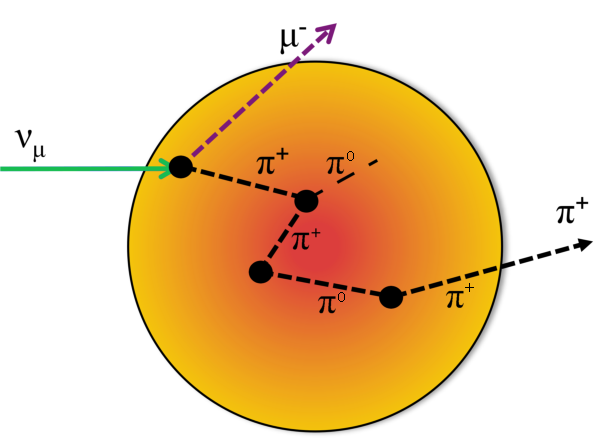
\includegraphics[width=0.3\textwidth, trim={0mm 0mm 0mm 0mm}, clip,page=1]{figures/niwg/diagrams/cascade}
	\caption{An example of a pion FSI cascade}
\end{figure}

The systematics are parameterised as the scattering probabilities for the different interaction processes at each microscopic step in the cascade. These are divided into absorption, pion production, quasi-elastic and charge exchange. Furthermore, the two latter are split into low and high energy regions, above and below the model transition at $p_\pi = 500\text{ MeV}$. For oscillation analyses using the 0$\pi$ topology, the absorption and elastic probabilities are most important since they can significantly bias energy reconstruction by removing pions from the reconstructed event. The prior values and uncertainties come from tuning to world scattering data: $\pi^+-^{12}C$ for the low energy and $\pi^\pm - ^{12}C$ for the high energy parameters.

Importantly, the pion rescattering probabilities are assumed to be independent, which is not correct. An extreme variation in the absorption probability will cause a pion to be absorbed, so the effect of the other parameters should be none. However this is not implemented as it was found to have a $\sim1\%$ effect on T2K run 2-4 data.

The nucleon interaction uncertainties are neglected since for water Cherenkov detector such as Super-Kamiokande, the nucleon threshold is rarely reached. However, when nucleons interact to produce pions these pions are propagated through the simulation and are subject to the above systematics.

\paragraph{Parameterisation}
The interaction parameters are parameterised as shapes or normalisations on an event-by-event basis. In the case of normalisations, an event gets an associated weight from normalisation parameters in the parameterisation (e.g. a CC coherent event on $^{12}C$ gets the CC coh. C parameter weight and no other: if the parameter is 1.5, the weight is 1.5). 

For shape parameters, each event can have associated one dimensional ``splines''\footnote{The implementation uses a ROOT \texttt{TSpline3} class}, which assumes all parameters have uncorrelated responses. The weights are pre-calculated through a reweighting routine which calculates the weight of parameter variation $x \rightarrow x'$, where $x$ is the nominal Monte Carlo parameter value and $x'$ is the new parameter value, as
\begin{equation}
	w(x\rightarrow x') = \frac{d^n\sigma(x')}{dX^n} / \frac{d^n\sigma(x)}{dX^n}
\end{equation}
for an $n$ dimensional cross-section calculation for $X$ dependent parameters. Similar to the pion FSI parameters, this is not strictly true since for example a simultaneous variation in $M_A^{RES}$ and $C_5^A$ is not equivalent to a variation in $M_A^{RES}$ followed by a variation of $C_5^A$. This is currently neglected in the analysis since the effect is sub-percent.

An example of three spline parameters, comparing a third order polynomial \texttt{TF1} implementation to a \texttt{TSpline3} implementation fitted to the discrete calculated parameter variations is shown in \autoref{fig:xsec_splines}.
\begin{figure}[h]
	\centering
	\begin{subfigure}[t]{0.32\textwidth}
		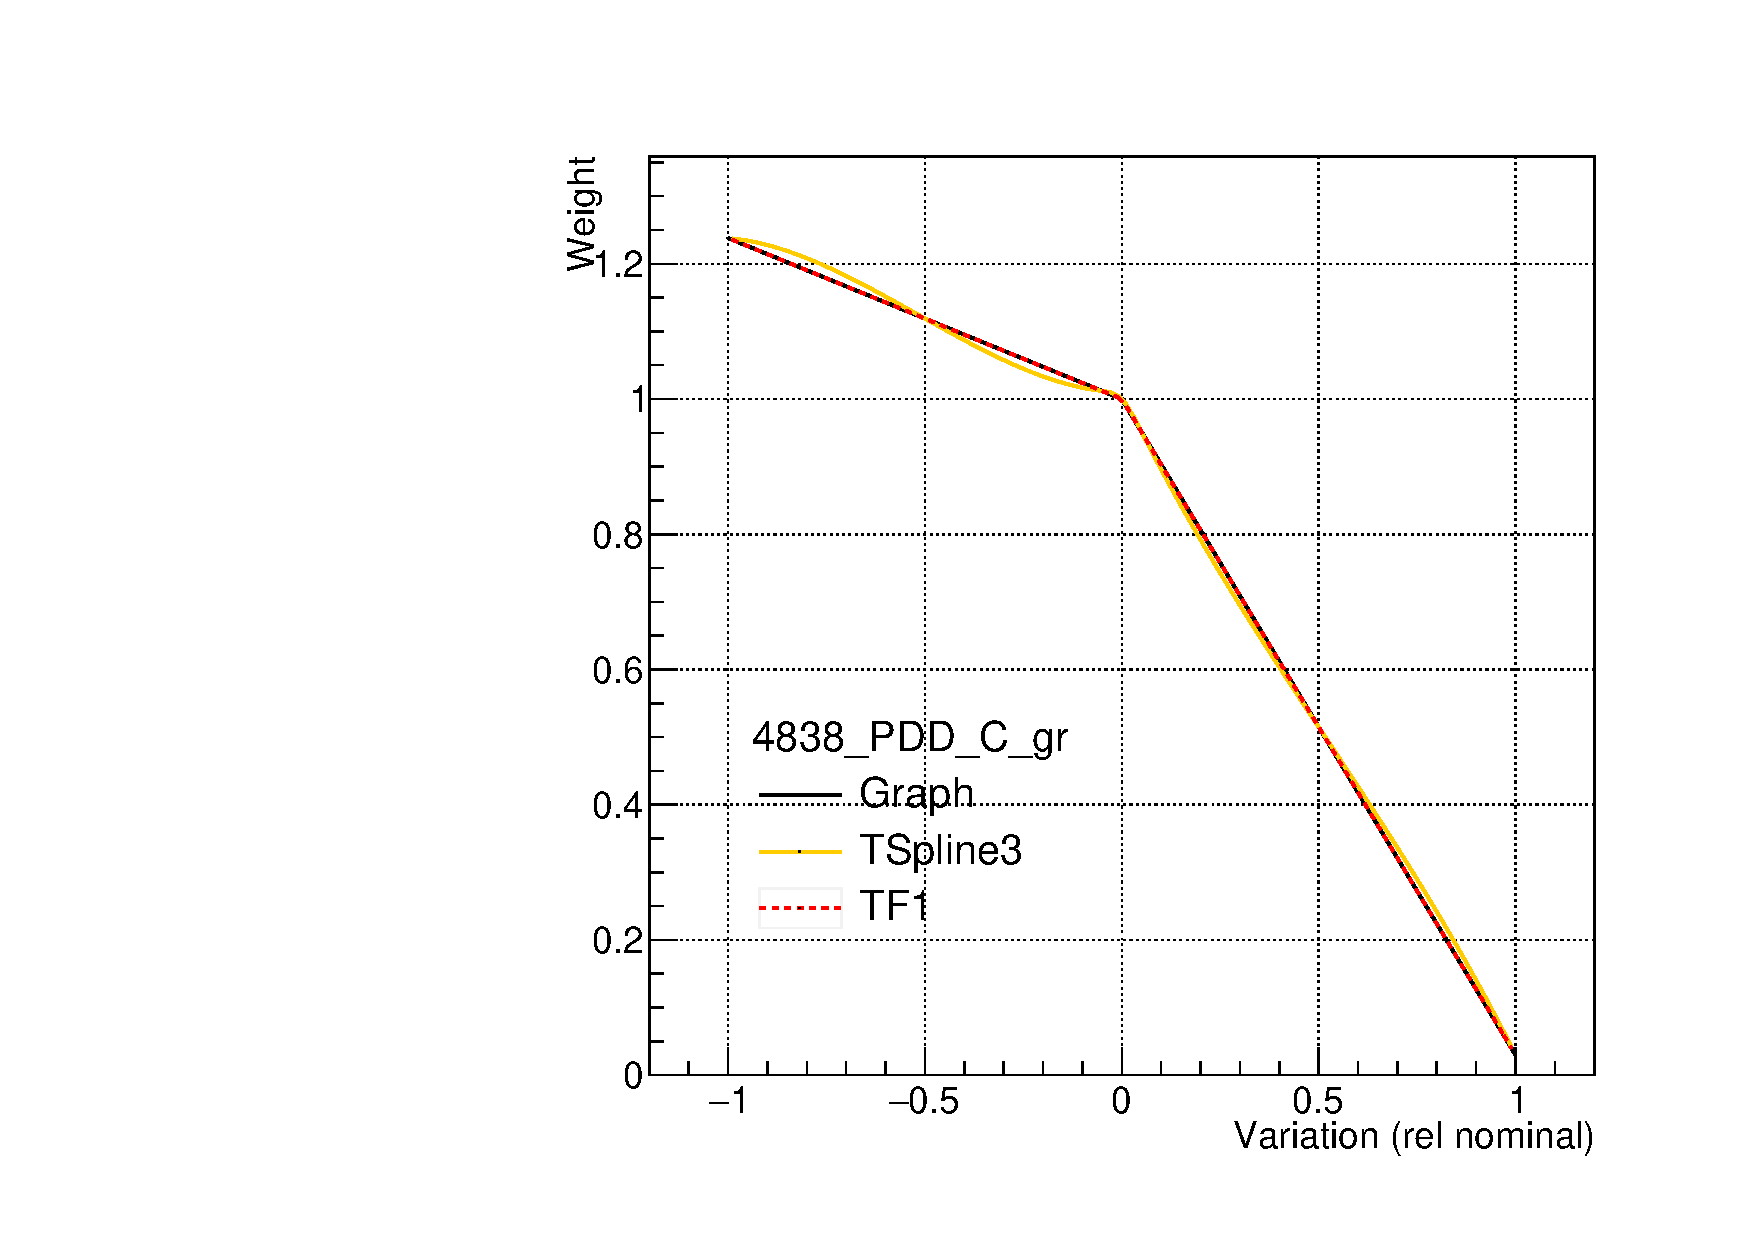
\includegraphics[width=\textwidth, trim={5mm 5mm 15mm 15mm}, clip,page=1]{figures/niwg/splines/pdd_c}
		\caption{2p2h shape C}
	\end{subfigure}
	\begin{subfigure}[t]{0.32\textwidth}
		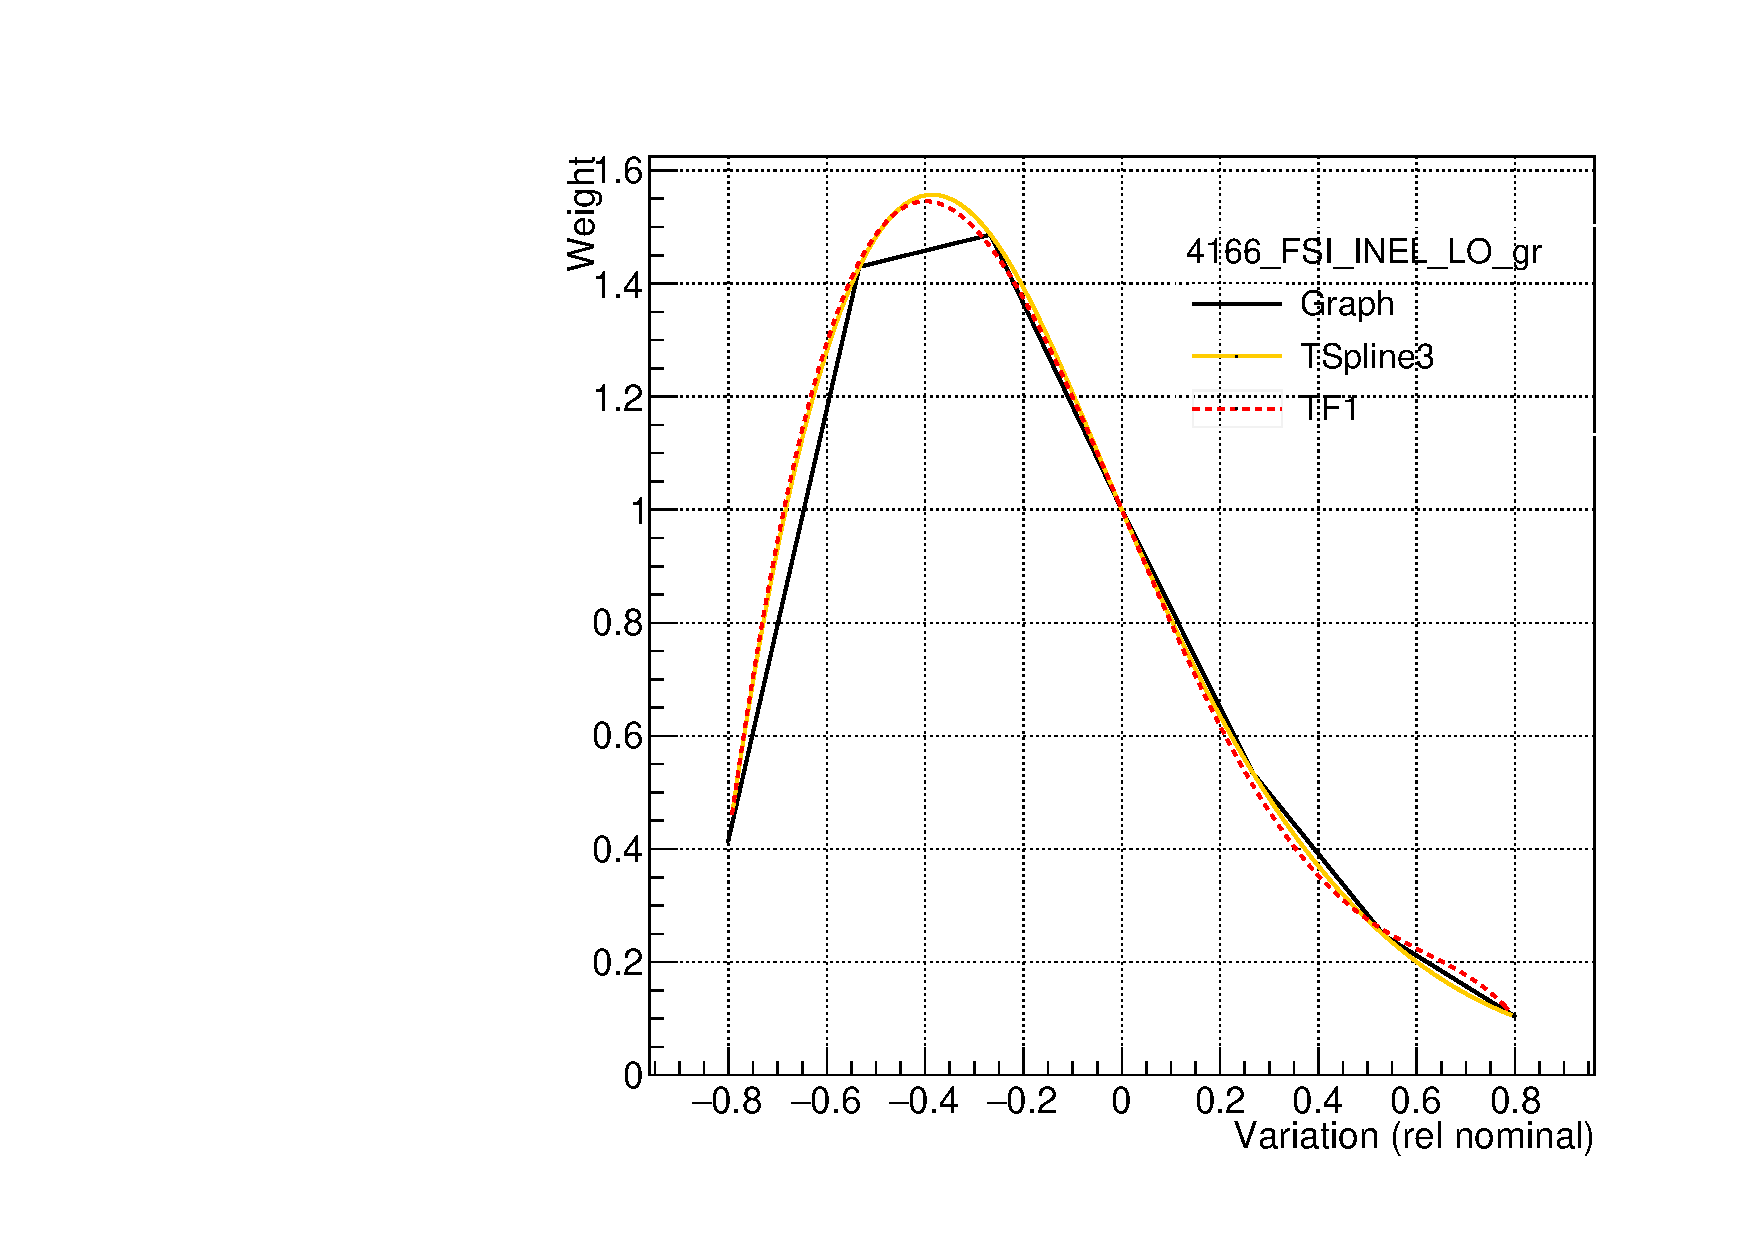
\includegraphics[width=\textwidth, trim={5mm 5mm 15mm 15mm}, clip,page=1]{figures/niwg/splines/fsi_inel_lo}
		\caption{FSI Inel. Lo}
	\end{subfigure}	
	\begin{subfigure}[t]{0.32\textwidth}
		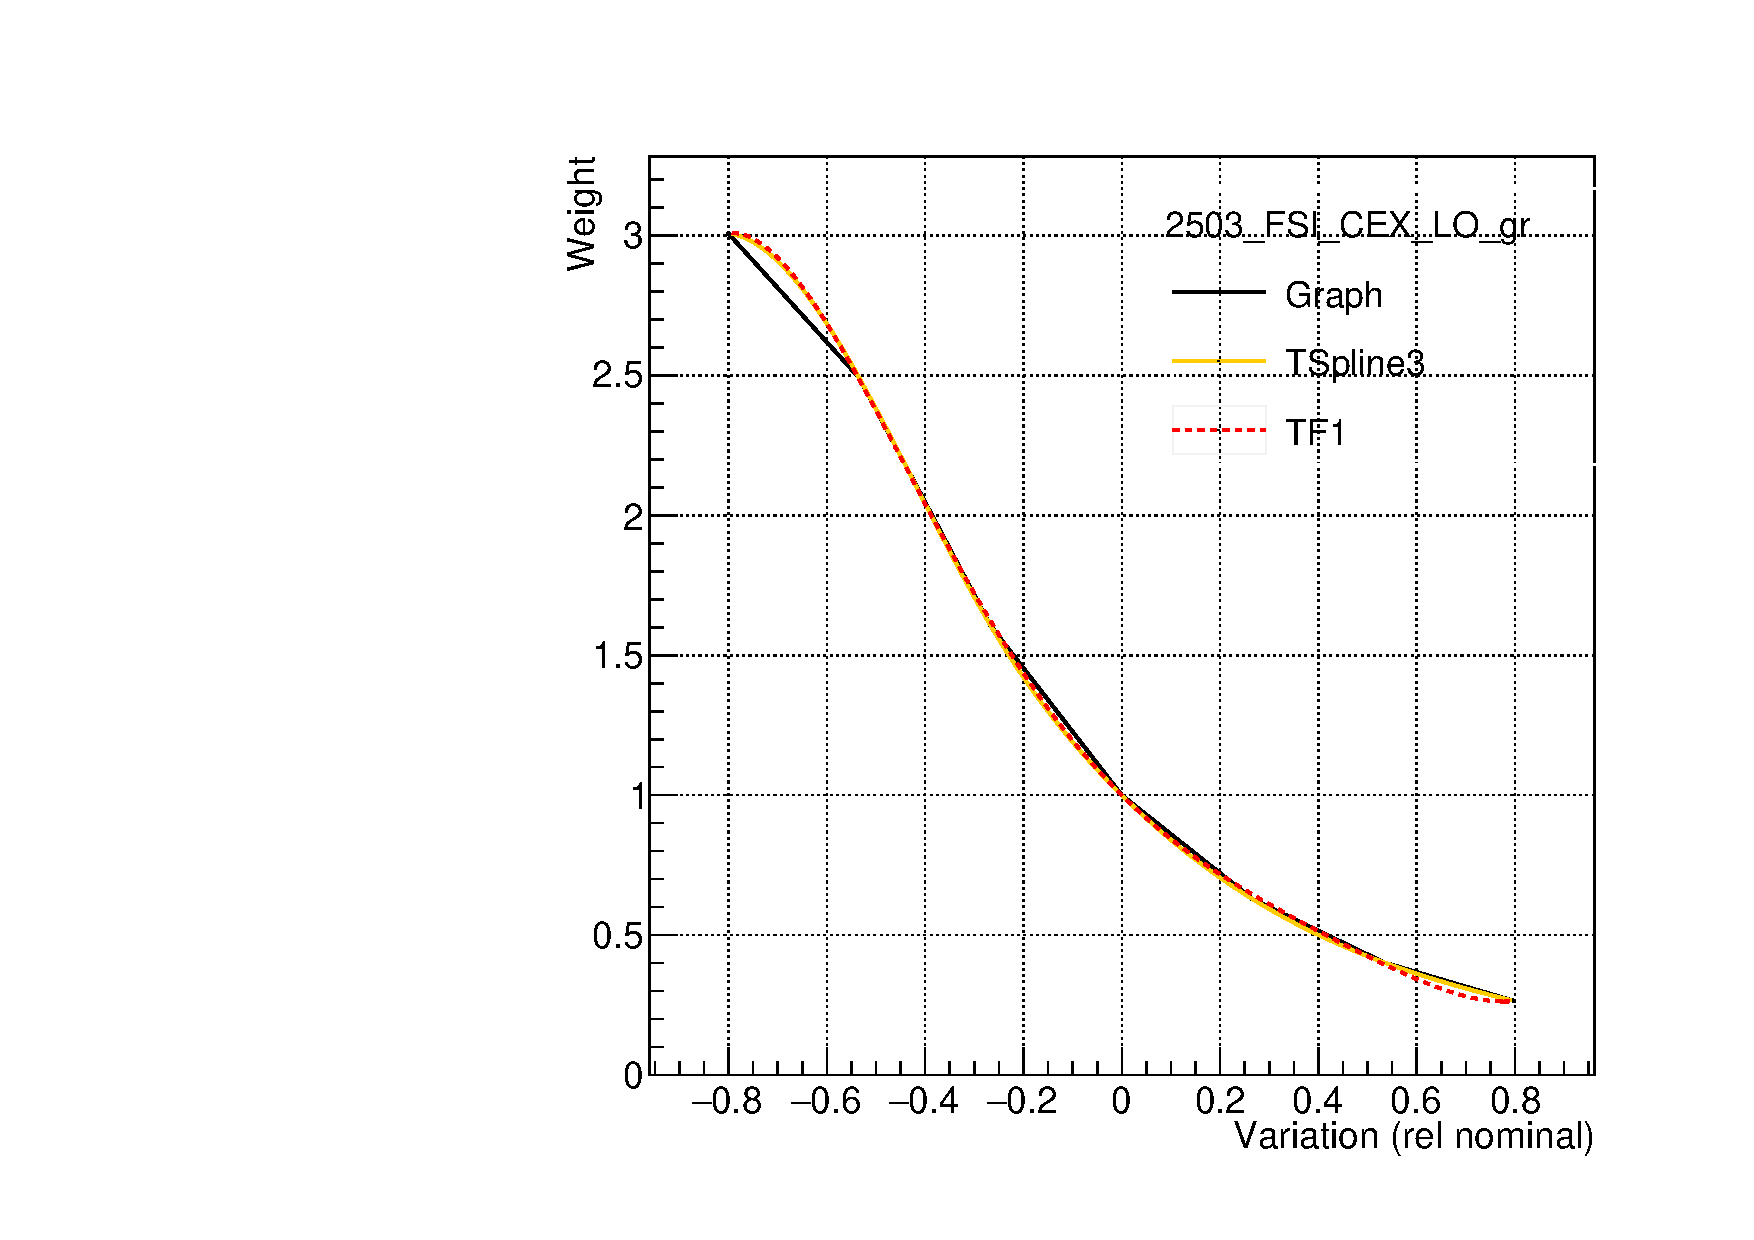
\includegraphics[width=\textwidth, trim={5mm 5mm 15mm 15mm}, clip,page=1]{figures/niwg/splines/fsi_cex_lo}
		\caption{FSI Cex. Lo}
	\end{subfigure}
\caption{A \texttt{TF1} and \texttt{TSpline3} shape implementation of three different shape parameters in the analysis}
\label{fig:xsec_splines}
\end{figure}

\paragraph{Covariance matrix}
\autoref{fig:xsec_cov_matrix_prior} shows the final $\sqrt{\textbf{V}}$ covariance and correlation matrix. Only a few parameters are correlated in the prior covariance matrix: the 2p2h shape C and O parameters (+0.55), the single pion production parameters (-0.8 to 0.10), the \nue(\nuebar)/\numu(\numubar) (-0.71), the CC coherent parameters (+1.00), and the pion FSI parameters (-1.00 to 1.00).
\begin{figure}[h]
	\begin{subfigure}[t]{0.49\textwidth}
		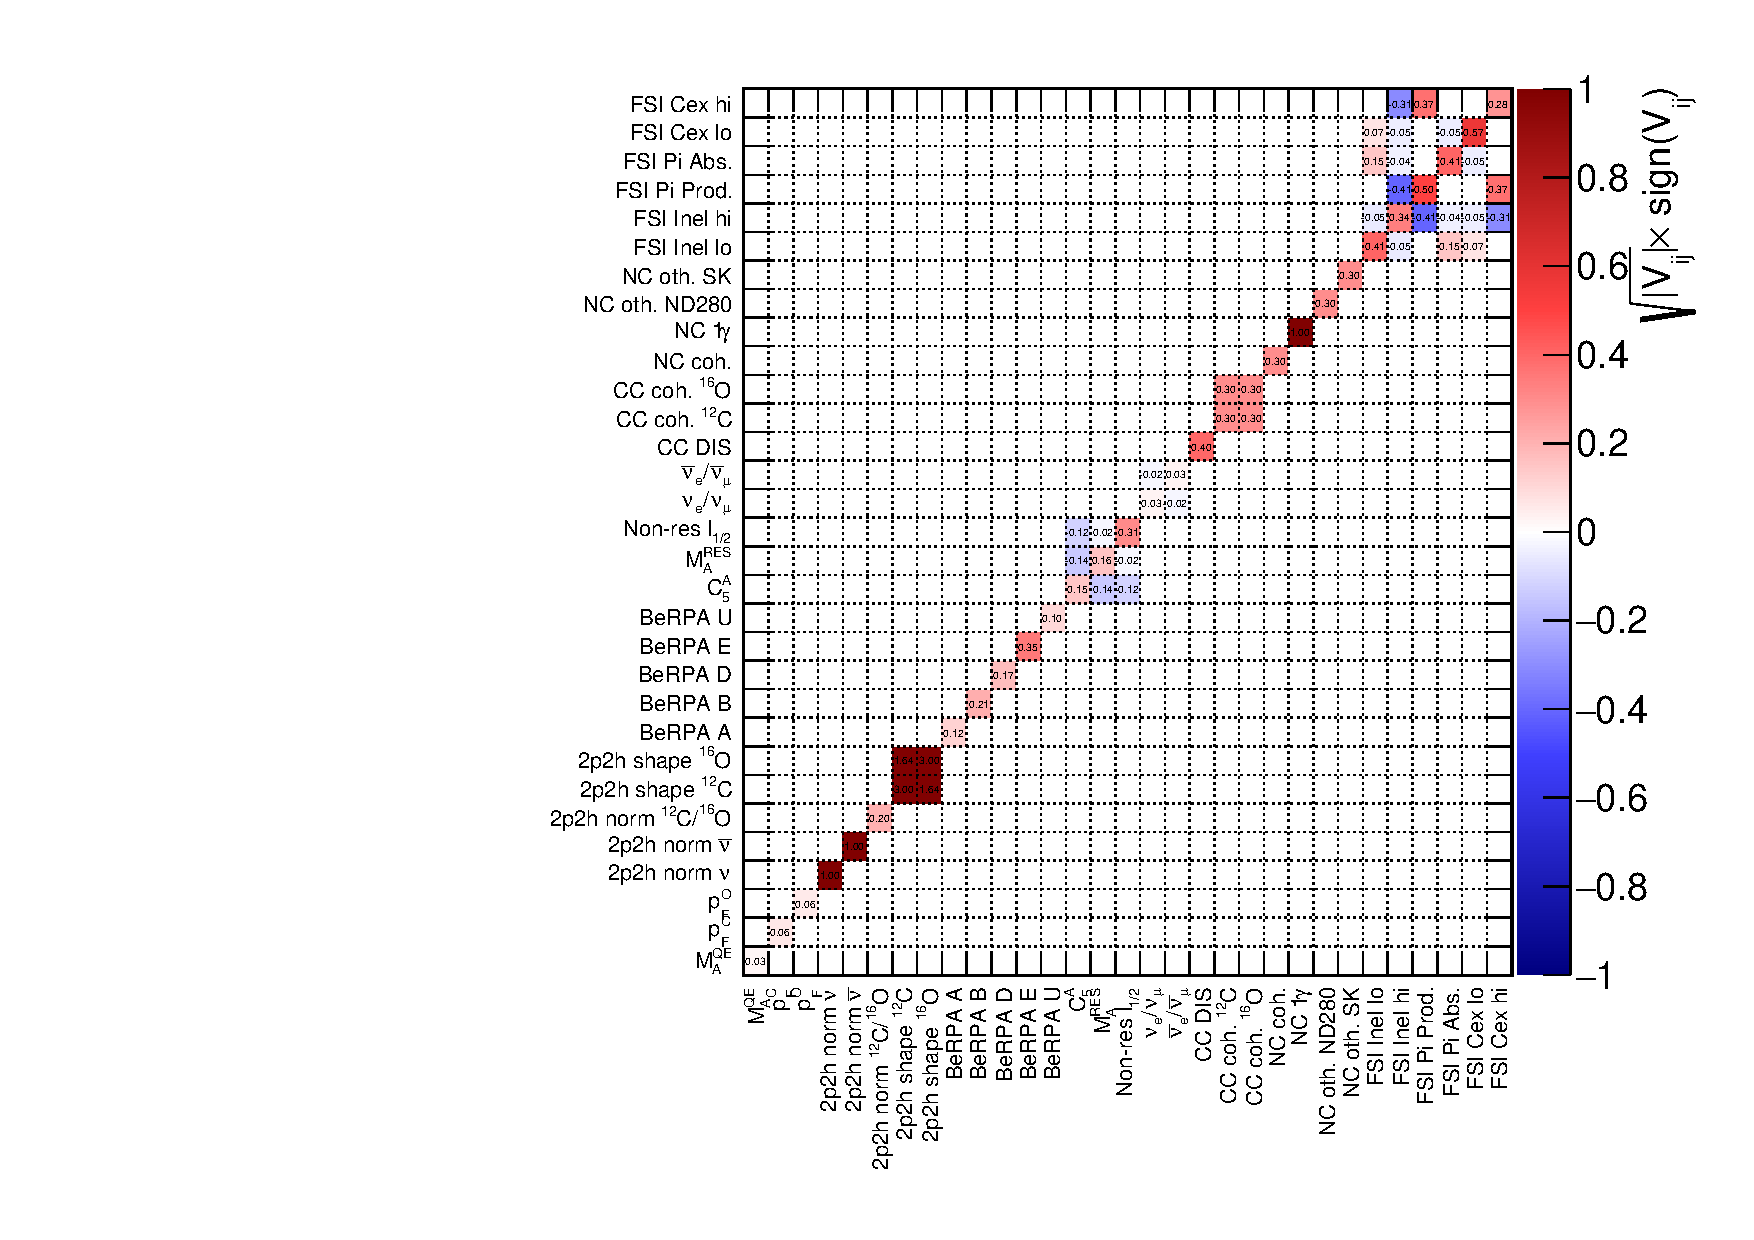
\includegraphics[width=\textwidth, trim={0mm 0mm 0mm 0mm}, clip, page=1] {figures/niwg/xsec_covariance_2017b_NOMINAL_v1_xseccov}
		\caption{$\sqrt{\text{Covariance}}$}
		\label{fig:xsec_cov_matrix_vij}
	\end{subfigure}
	\begin{subfigure}[t]{0.49\textwidth}
		\includegraphics[width=\textwidth, trim={0mm 0mm 0mm 0mm}, clip, page=2] {figures/niwg/xsec_covariance_2017b_NOMINAL_v1_xseccov}
		\caption{Correlation}
	\end{subfigure}
	\caption{Interaction covariance matrix provided as the prior}
	\label{fig:xsec_cov_matrix_prior}
\end{figure}

Note that some of the errors in \autoref{fig:xsec_cov_matrix_vij} do not include the flat priors on $M_A^{QE}, p_F$ and that BeRPA U is fixed. Furthermore, the errors are relative the priors: e.g. the error on $p_F^C$ is not 6 MeV but rather $217\times0.06=13\text{ MeV}$.

\begin{table}
	\begin{tabular}{l | c c c c }
		\hline
		\hline
		Parameter & Nominal & Error & Prior shape & Parameter type \\
		\hline
		$M_A^{QE}$ & 1.21 GeV & 0-10 & Flat & Shape \\
		$M_A^{QE} H$ & 1.03 GeV & 0 & --- & Shape \\
		$p_F^C$ & 217 MeV & 31 MeV & Flat & Shape \\
		$p_F^O$ & 225 MeV & 31 MeV & Flat & Shape \\
		2p2h norm $\nu$ & 1.0 & 1.0 & Flat & Norm. \\
		2p2h norm $\bar{\nu}$ & 1.0 & 1.0 & Flat & Norm. \\
		2p2h norm C to O & 1.0 & 0.2 & Gauss & Norm. \\
		2p2h shape C & 1.0 & 3.0 & Gauss & Shape \\
		2p2h shape O & 1.0 & 3.0 & Gauss & Shape \\ 
		BeRPA A & 0.59 & 0.118 & Gauss & Shape \\
		BeRPA B & 1.05 & 0.210 & Gauss & Shape \\
		BeRPA D & 1.13 & 0.170 & Gauss & Shape \\
		BeRPA E & 0.88 & 0.352 & Gauss & Shape \\
		BeRPA U & 1.20 & --- & --- & --- \\
		\hline
		
		\hline
		\hline
	\end{tabular}
\end{table}